
%%  This Beamer template was created by Cameron Bracken.
%%  Anyone can freely use or modify it for any purpose
%%  without attribution.
%%
%%  Last Modified: January 9, 2009
%%

% removed compress key option to documentclass 
\documentclass[xcolor=x11names,compress,ignorenonframetext,10pt]{beamer}

%% General document %%%%%%%%%%%%%%%%%%%%%%%%%%%%%%%%%%
\usepackage{booktabs,multirow}
\usepackage{bm}
\usepackage{graphicx}
\usepackage{tikz}
\usepackage[abs]{overpic}
\usepackage{pict2e}

%\usetikzlibrary{decorations.fractals}

\renewcommand{\star}{*}

\DeclareMathOperator*{\argmin}{arg\,min}
\DeclareMathOperator{\gap}{gap}

\def\rf{\mathrm{F}}
\def\bigbar{\big\|}
\def\pinv{\dagger}
\def\transp{^T}
% 
\newcommand{\samats}[1]{\ensuremath{\mathbb{M}^{#1}_{\mathrm{sa}}}}
\newcommand{\s}{\sigma} % singular values
\newcommand{\asymO}[1]{\ensuremath{\mathop{\text{O}}\!\left(#1\right)}}
\DeclareMathOperator{\sgn}{sgn}

\newcommand{\norm}[1]{\ensuremath{\left\|#1\right\|}}
\newcommand{\supoverinfball}{\ensuremath{\max_{\infnorm{\mat{u}} = 1}}}
\newcommand{\supovertball}{\ensuremath{\max_{\norm{\mat{u}}_2 = 1}}}
\newcommand{\supoverqball}{\ensuremath{\max_{\qnorm{\mat{u}} = 1}}}
\newcommand{\eqqcolon}{=\mathrel{\mathop:}} %this may not be what I want, =:

\newcommand{\mat}[1]{\ensuremath{\mathbf{#1}}}
\renewcommand{\vec}[1]{\ensuremath{\mathbf{#1}}}
\newcommand{\e}{\ensuremath{\mathrm{e}}}
\newcommand{\E}{\ensuremath{\mathbb{E}}}
\newcommand{\Prob}[1]{\ensuremath{\mathbb{P}\left\{#1\right\}}}
\newcommand{\CondProb}[2]{\ensuremath{\mathbb{P}\left\{#1 \,\left|\, #2 \right.\right\}}}
\newcommand{\lnorm}[2]{\ensuremath{\left\| #2 \right\|_{L_{#1}}}}
\newcommand{\lipnorm}[1]{\ensuremath{\left\| #1 \right\|_\Pi}}
\newcommand{\R}{\ensuremath{\mathbb{R}}}
\newcommand{\Cfield}{\ensuremath{\mathbb{C}}}
\newcommand{\randcon}{\ensuremath{\Psi}}
\newcommand{\indicator}[1]{\ensuremath{\mathbb{1}\left\{#1\right\}}}

\newcommand{\xiNorm}[1]{\ensuremath{\left\|#1\right\|_\xi}}
\newcommand{\TNorm}[1]{\ensuremath{\left\|#1\right\|_2}}
\newcommand{\TNormS}[1]{\ensuremath{\left\|#1\right\|_2^2}}
\newcommand{\FNorm}[1]{\ensuremath{\left\|#1\right\|_\mathrm{F}}}
\newcommand{\FNormS}[1]{\ensuremath{\left\|#1\right\|_\mathrm{F}^2}}
\newcommand{\VTNorm}[1]{\ensuremath{\left\|#1\right\|_2}}
\newcommand{\VTNormS}[1]{\ensuremath{\left\|#1\right\|_2^2}}
\newcommand{\tracenorm}[1]{\ensuremath{\trace\left(#1\right)}}

\newcommand{\xinorm}[1]{\ensuremath{\big\|#1\big\|_\xi}}
\newcommand{\xinorms}[1]{\ensuremath{\big\|#1\big\|_\xi^2}}
\newcommand{\snorm}[1]{\ensuremath{\left\|#1\right\|_2}}
\newcommand{\snorms}[1]{\ensuremath{\big\|#1\big\|_2^2}}
\newcommand{\fnorm}[1]{\ensuremath{\left\|#1\right\|_{\mathrm{F}}}}
\newcommand{\fnorms}[1]{\ensuremath{\big\|#1\big\|_{\mathrm{F}}^2}}
\newcommand{\mcnorm}[1]{\ensuremath{\big\|#1\big\|_{\mathrm{mc}}}}
\newcommand{\mcnorms}[1]{\ensuremath{\big\|#1\big\|_{\mathrm{mc}}^2}}

\newcommand{\pnorm}[1]{\ensuremath{\left\|#1\right\|_p}}
\newcommand{\qnorm}[1]{\ensuremath{\left\|#1\right\|_q}}
\newcommand{\infnorm}[1]{\ensuremath{\left\|#1\right\|_\infty}}
\newcommand{\infonorm}[1]{\ensuremath{\left\|#1\right\|_{\infty\rightarrow 1}}}
\newcommand{\inftnorm}[1]{\ensuremath{\left\|#1\right\|_{\infty\rightarrow 2}}}
\newcommand{\onetwonorm}[1]{\ensuremath{\left\|#1\right\|_{1 \rightarrow 2}}}
\newcommand{\twoinfnorm}[1]{\ensuremath{\left\|#1\right\|_{2 \rightarrow \infty}}}
\newcommand{\smalltwoinfnorm}[1]{\ensuremath{\|#1\|_{2 \rightarrow \infty}}}
\newcommand{\infone}{\ensuremath{\infty\!\rightarrow\!\!1}}
\newcommand{\inftwo}{\ensuremath{\infty\!\rightarrow\!\!2}}
\newcommand{\infp}{\ensuremath{\infty\!\rightarrow\!p}}
\newcommand{\twoinf}{\ensuremath{2\!\!\rightarrow\!\!\infty}}
\newcommand{\colnorm}[1]{\ensuremath{\left\|#1\right\|_{\mathrm{col}}}}
\newcommand{\rownorm}[1]{\ensuremath{\left\|#1\right\|_{\text{\rmfamily{row}}}}}
\newcommand{\cutnorm}[1]{\ensuremath{\left\|#1\right\|_{\text{\rmfamily{C}}}}}

\newcommand{\F}{F}
\newcommand{\lambdamax}[1]{\ensuremath{\lambda_{\mathrm{max}}\left(#1\right)}}
\newcommand{\lambdamin}[1]{\ensuremath{\lambda_{\mathrm{min}}\left(#1\right)}}
\newcommand{\sigmamin}[1]{\ensuremath{\sigma_{\mathrm{min}}\left(#1\right)}}
\newcommand{\sigmamax}[1]{\ensuremath{\sigma_{\mathrm{max}}\left(#1\right)}}
\newcommand{\Isom}[2]{\ensuremath{\mathbb{V}_{#1}^{#2}}}
\DeclareMathOperator{\tr}{tr}
\DeclareMathOperator{\trace}{Tr}
\DeclareMathOperator{\rank}{rank}
\DeclareMathOperator{\var}{Var}
\newcommand{\trbrace}[1]{\ensuremath{\tr\left(#1\right)}}
\newcommand{\trexp}[1]{\ensuremath{\tr\exp\left(#1\right)}}
\newcommand{\const}[1]{\ensuremath{\mathrm{#1}}}

%\newtheorem{thm}{Theorem}[chapter]
%\newtheorem{prop}[thm]{Proposition}
%\newtheorem{lemma}[thm]{Lemma}
%\newtheorem{cor}[thm]{Corollary}
%\newtheorem{defn}[thm]{Definition}

%\theoremstyle{remark}
%\newtheorem{remark}[thm]{Remark}


% Bunch of stuff from the SRHT paper, need to eliminate redundancy and fold in
\newcommand{\Probab}[1]{\mbox{}{\mathbb{P}}\left(#1\right)}
\newcommand{\Exp}{\mbox{}{\mathbf{E}}}
\newcommand{\Expect}[1]{\mbox{}{\mathbb{E}}\left[#1\right]}
\newcommand{\Varnce}[1]{\mbox{}{\mathbf{Var}}\left[#1\right]}
\newcommand{\Trace }[1]{\mbox{}{\mathrm{Tr}}\left(#1\right)}
\newcommand{\diag  }[1]{\mbox{}{\textrm{diag}}\left(#1\right)}
\newcommand{\Sqrt  }[1]{\mbox{}\left(#1\right)^{1/2}}
\newcommand{\Qdrt  }[1]{\mbox{}\left(#1\right)^{1/4}}
\newcommand{\FNormB }[1]{\mbox{}\left\|#1\right\|_{\mathrm{F}}  }
\newcommand{\FNormBS}[1]{\mbox{}\left\|#1\right\|_{\mathrm{F}}^2}
\newcommand{\FNormF}[1]{\mbox{}\|#1\|_\mathrm{F}^4}
\newcommand{\FNormQ}[1]{\mbox{}\left\|#1\right\|_\mathrm{F}^4}
\newcommand{\TNormB }[1]{\mbox{}\left\|#1\right\|_2  }
\newcommand{\TNormBS}[1]{\mbox{}\left\|#1\right\|_2^2}
\newcommand{\TNormF}[1]{\mbox{}\|#1\|_2^4}
\newcommand{\TNormQ}[1]{\mbox{}\left\|#1\right\|_2^4}
\newcommand{\XNormB }[1]{\mbox{}\left\|#1\right\|_{\xi}  }
\newcommand{\XNormBS}[1]{\mbox{}\left\|#1\right\|_{\xi}^2}
\newcommand{\XNorm }[1]{\mbox{}\|#1\|_{\xi}  }
\newcommand{\XNormS}[1]{\mbox{}\|#1\|_{\xi}^2}
\newcommand{\PNorm }[1]{\mbox{}\|#1\|_{p}  }
\newcommand{\PNormS}[1]{\mbox{}\|#1\|_{p}^2}
\newcommand{\XNormQ}[1]{\mbox{}\left\|#1\right\|_{\xi}^4}
\newcommand{\VTNormQ}[1]{\mbox{}\left|#1\right|^4}
\newcommand{\VTTNorm }[1]{\mbox{}\left|#1\right|_2  }
\newcommand{\VTTNormS}[1]{\mbox{}\left|#1\right|_2^2}
\newcommand{\VTTNormQ}[1]{\mbox{}\left|#1\right|_2^4}
\newcommand{\MCNorm}[1]{\mbox{}\|#1\|_{1 \rightarrow 2}}
\newcommand{\MCNormS}[1]{\mbox{}\|#1\|_{1 \rightarrow 2}^2}
\newcommand{\INorm}[1]{\mbox{}\|#1\|_\infty}

\newcommand{\qedsymb}{\hfill{\rule{2mm}{2mm}}}

\newcommand{\dvc}{\ensuremath{d_{\small \sf VC}}}
\newcommand{\abs }[1]{\left|#1\right|}
\newcommand{\EE}[1]{\ensuremath{\mathbb{E}\left[#1\right] } }
\newcommand{\condE}[2]{\ensuremath{\mathbb{E}\left[#2 \,\left|\, #1 \right.\right]}}

\def\gammab{{\bm{\gamma}}}
\def\kappab{{\bm{\kappa}}}
\def\sig{{\bm{\Sigma}}}
\def\sigplus{{\bm{\Sigma}^{+}}}
\def\siginv{{\bm{\Sigma}^{-1}}}
\def\bet{{\bm{\beta}}}
\def\one{{\bm{1}}}
\def\exp{\ensuremath{\mathrm{exp}}}
\def\rank{\mathrm{rank}}
\newcommand{\stablerank}[1]{\operatorname{sr}\left(#1\right)}

%\def\cond{\hbox{\rm \mathbf{k}}}

\def\col{\hbox{\mathrm{col}}}
\def\ker{\hbox{\mathrm{ker}}}
\def\ahat{{\hat\a}}
\def\b{{\mathbf b}}
%\def\e{{\mathbf e}}
\def\expe{\mathrm{e}}
\def\q{{\mathbf q}}
\def\rb{{\mathbf r}}
%\def\s{{\mathbf s}}
%\def\u{{\mathbf u}}
\def\v{{\mathbf v}}
\def\x{{\mathbf x}}
\def\y{{\mathbf y}}
\def\z{{\mathbf z}}
\def\h{{\mathbf h}}
\def\d{{\mathbf \delta}}
\def\xhat{{\hat\x}}
\def\yhat{{\hat\y}}
\def\A{\matA}
\def\B{\matB}
%\def\C{\matC}
\def\Ahat{\hat\matA}
\def\Atilde{\tilde\matA}
\def\Btilde{\tilde\matB}
\def\Stilde{\tilde\matS}
\def\Utilde{\tilde\matU}
\def\Vtilde{\tilde\matV}
%\def\E{{\cl E}}
\def\G{{\cl G}}
\def\hset{{\cl H}}
\def\Q{{\bm{Q}}}
\def\U{{\bm{U}}}
\def\V{{\bm{V}}}
\def\win{\hat{\w}}
\def\wopt{\w^*}
\def\matAhat{\hat\mat{A}}
\def\matA{\mat{A}}
\def\matB{\mat{B}}
\def\matC{\mat{C}}
\def\matD{\mat{D}}
\def\matE{\mat{E}}
\def\matG{\mat{G}}
\def\matH{\mat{H}}
\def\matI{\mat{I}}
\def\matF{\mat{F}}
\def\matM{\mat{M}}
\def\matP{\mat{P}}
\def\matQ{\mat{Q}}
\def\matR{\mat{R}}
\def\matS{\mat{S}}
\def\matT{\mat{T}}
\def\matU{\mat{U}}
\def\matV{\mat{V}}
\def\matW{\mat{W}}
\def\matX{\mat{X}}
\def\matXopt{\mat{X}_{\mathrm{opt}}}
\def\matY{\mat{Y}}
\def\matZ{\mat{Z}}
\def\matSig{\boldsymbol{\Sigma}}
\def\matTh{\boldsymbol{\Theta}}
\def\matOmega{\boldsymbol{\Omega}}
\def\matPsi{\mat{\Psi}}
\def\matGam{\mat{\Gamma}}
\def\boldPi{\boldsymbol{\Pi}}
\def\w{{\mathbf{w}}}
\def\ein{{\cl E_{\text{\mathrm{in}}}}}
\def\eout{{\cl E}}
\def\scl{{\textsc{l}}}
\def\scu{{\textsc{u}}}
\def\phiu{{\overline{\phi}}}
\def\psiu{{\overline{\psi}}}
\def\phil{{\underbar{\math{\phi}}}}
%\DeclareMathSymbol{\Prob}{\mathbin}{AMSb}{"50}
%\DeclareMathSymbol{\Exp}{\mathbin}{AMSb}{"45}
\newcommand\remove[1]{}

\def\nnz{{ \mathrm nnz }}

\usepackage[ruled,vlined]{algorithm2e}
\usepackage{float}
\usepackage[noend]{algpseudocode}

% next three are from craftmaps
%\usepackage{algorithm}
\usepackage{xcolor,colortbl}
%\usepackage{caption}
\usepackage{algcompatible}
%\usepackage{subfig}
%%%%%%%%%%%%%%%%%%%%%%%%%%%%%%%%%%%%%%%%%%%%%%%%%%%%%%

\usepackage{etoolbox}
\let\bbordermatrix\bordermatrix
\patchcmd{\bbordermatrix}{8.75}{4.75}{}{}
\patchcmd{\bbordermatrix}{\left(}{\left[}{}{}
\patchcmd{\bbordermatrix}{\right)}{\right]}{}{}

\definecolor{dgreen}{rgb}{0.,0.6,0.}

%% Beamer Layout %%%%%%%%%%%%%%%%%%%%%%%%%%%%%%%%%%
\useoutertheme[subsection=false,shadow]{miniframes}
\useinnertheme{default}
\usefonttheme{serif}
\usepackage{palatino}

\setbeamerfont{title like}{shape=\scshape}
\setbeamerfont{frametitle}{shape=\scshape}
\setbeamerfont{headline}{size=\normalsize}

\setbeamercolor*{lower separation line head}{bg=DeepSkyBlue4} 
\setbeamercolor*{normal text}{fg=black,bg=white} 
\setbeamercolor*{alerted text}{fg=red} 
\setbeamercolor*{example text}{fg=black} 
\setbeamercolor*{structure}{fg=black} 
 
\setbeamercolor*{palette tertiary}{fg=black,bg=black!10} 
\setbeamercolor*{palette quaternary}{fg=black,bg=black!10} 

\setbeamercolor{block title}{bg=blue!30, fg=black}
\setbeamercolor{block body}{bg=blue!10, fg=black}

\beamertemplatenavigationsymbolsempty

\setbeamertemplate{footline}[frame number]
% \setbeamertemplate{headline}{%
%   \hbox{%
%     \begin{beamercolorbox}[wd=\paperwidth,ht=2.5ex,dp=1.125ex]{palette primary}%
%       \insertsectionnavigationhorizontal{\paperwidth}{}{\hskip0pt plus1filll}
%     \end{beamercolorbox}
%   }
% }

\renewcommand{\(}{\begin{columns}}
\renewcommand{\)}{\end{columns}}
\newcommand{\<}[1]{\begin{column}{#1}}
\renewcommand{\>}{\end{column}}
%%%%%%%%%%%%%%%%%%%%%%%%%%%%%%%%%%%%%%%%%%%%%%%%%%

%\DeclareMathOperator{\gap}{gap}

\def\refcolor{DodgerBlue4}
\newcommand{\refer}[1]{({\color{\refcolor}#1})}
\newcommand{\redemphasis}[1]{\textbf{\textit{\textcolor{red}{#1}}}}
\newcommand{\greenemphasis}[1]{\textbf{\textit{\textcolor{dgreen}{#1}}}}

\newcommand{\alertline}{%
 \usebeamercolor[fg]{normal text}%
 \only{\usebeamercolor[fg]{alerted text}}}
\begin{document}


%%%%%%%%%%%%%%%%%%%%%%%%%%%%%%%%%%%%%%%%%%%%%%%%%%%%%%
%%%%%%%%%%%%%%%%%%%%%%%%%%%%%%%%%%%%%%%%%%%%%%%%%%%%%%
\begin{frame}
  \title{Linear and Nonlinear Low-Rank Approximations}
  \subtitle{in theory and practice}

\author{
  \vskip2em
	\begin{tabular}[h]{c}
	Alex Gittens \\
  International Computer Science Institute (ICSI) \\
  Department of Statistics and AMPLab \\
  University of California, Berkeley
	\end{tabular}
}
\date{
  RPI CS Colloquium \\
  May 5, 2016
}
\maketitle
\end{frame}

%%%%%%%%%%%%%%%%%%%%%%%%%%%%%%%%%%%%%%%%%%%%%%%%%%%%%%
%%%%%%%%%%%%%%%%%%%%%%%%%%%%%%%%%%%%%%%%%%%%%%%%%%%%%%
\section{Outline}
 \begin{frame}{Outline}
   Low-rank matrix approximation is a fundamental tool, used for multiple reasons: 
     noise elimination, computational tractability, statistical modeling, ....

     \vskip1em
     We consider the following instances of low-rank approximation:
     \begin{itemize}
       \item \textcolor{red}{Randomized SPSD Sketching} for fast linear low-rank approximation
       \item \textcolor{dgreen}{Polynomial Random Features} for fast approximate polynomial kernel learning
       \item \textcolor{red}{Word2Vec} for semantically meaningful word embeddings
       \item The performance of \textcolor{dgreen}{Low-rank approximation algorithms in Spark}
     \end{itemize}

   \end{frame}
%
%   \begin{frame}
%     We ask:
%   \begin{itemize}
%     \item What guarantees are available for these low-rank approximations? 
%     \item How well do they perform in practice?
%   \end{itemize}
%
%  Who is interested in these approximations and our guarantees?
%  \begin{itemize}
%   \item The {\color{dgreen} numerical linear algebra community} wants high quality approximations
%   with very low failure rates and low communication cost.
%   \item The {\color{dgreen} machine learning community} wants approximations whose errors are on par
%   with modeling inaccuracies and the imprecision of the data
%   \item The {\color{dgreen} optimization community} is interested in varying levels of quality.
%   \item The {\color{dgreen} theoretical computer science community} is interested in understanding the
%   behavior of these algorithms.
%  \end{itemize}
% \end{frame}
%
%%%%%%%%%%%%%%%%%%%%%%%%%%%%%%%%%%%%%%%%%%%%%%%%%%%%%%
%%%%%%%%%%%%%%%%%%%%%%%%%%%%%%%%%%%%%%%%%%%%%%%%%%%%%%
\section{SPSD Sketches}

\begin{frame}
\vfill
\begin{beamercolorbox}[center]{}
\Large \textsc{SPSD Sketches}
\end{beamercolorbox}
\vfill
\end{frame}

\begin{frame}
 \begin{block}{Our basic task}
   $\matA \in \R^{n \times n}$ is a \emph{huge} symmetric positive-semidefinite matrix. Given $k \ll n,$ we
  would like a low-rank approximation to $\matA$ with rank about $k$.
 \end{block}

 \begin{enumerate}
  \item This abstract problem is ubiquitous in data processing tasks: statistical analysis, spectral clustering,
  kernel methods, optimization, ...
\item Traditional deterministic approaches (via truncated EVD, Krylov methods, etc.)
  cost at least $\mathrm{O}(n^2 k\log n)$ operations, and can have high communications costs.
 \end{enumerate}

\end{frame}

\begin{frame}
 One can consider using randomness to assist in the design of time and communication efficient algorithms
 for finding low-rank approximations of large matrices. 
 \vspace{0.7em}
 
 We give new error bounds for 
 ``sketching'' schemes for symmetric positive semidefinite matrices.
 
\begin{block}{Our objective}
 Determine how the errors of SPSD sketches in the spectral, Frobenius, and trace norms compare with the errors of $\matA_k,$ the 
 best rank-$k$ approximation to $\matA.$
\end{block}

\end{frame}
%%%%%%%%%%%%%%%%%%%%%%%%%%%%%%%%%%%%%%%%%%%%%%%%%%%%%%
%%%%%%%%%%%%%%%%%%%%%%%%%%%%%%%%%%%%%%%%%%%%%%%%%%%%%%

% \begin{frame}{Optimal rank-$k$ approximation}
% Fix $\matA \in \R^{m \times n}$ with $m \geq n.$
% 
% The most accurate rank-$k$ approximation in the spectral and Frobenius norms
% \[
%  \matA_k = \underset{%
%                \substack{%
%                  \matM \in \R^{m \times n} \\ 
%                  \operatorname{rank}(\tilde{\matA}) \leq k}}%
%            {\operatorname{argmin}}  
%            \|\matA - \matM\|_\xi, \quad \text{ for $\xi \in \{2, \mathrm{F}\}$}.
% \]
% can be computed in $\mathrm{O}(mn^2)$ time via the Singular Value Decomposition (SVD): if\vspace{-1em}
% \[
% \mat{A} = \mat{U} \matSig \mat{V}\transp = \bbordermatrix{%
% &^k \vspace{-0.75ex} & \!\!^{n-k}  \hspace{1ex}\cr
% & \vspace{0.25ex} \mat{U}_1 \hspace{-2ex} & \mat{U}_2 
% }
% \bbordermatrix{%
% & \vspace{-0.75ex} ^k &\!\!^{n-k} \hspace{1ex}\cr
% & \matSig_1 & \cr
% & \vspace{0.5ex} & \matSig_2 
% }
% \left[
% \begin{matrix}
% \mat{V}_1\transp \\
% \mat{V}_2\transp  
% \end{matrix}
% \right]
% \]
% then $\matA_k = \matU_1 \matSig_1 \matV_1\transp.$
% 
% \end{frame}

% \begin{frame}
%  We measure the approximation accuracies relative to those of $\matA_k,$ obtained
%  from a rank-$k$ truncated SVD of $\matA.$
%  
%  \begin{itemize}
%   \item An approximation $\matM$ satisfies a \emph{relative-error bound} if
%            \[
%            \|\matA - \matM\|_\xi \leq (1 + \epsilon) \|\matA - \matA_k\|_\xi 
%            \]
%   for an $\epsilon > 0.$
%   
%   \item It satisfies an \emph{additive-error bound} if 
%            \[
%             \|\matA - \matM\|_\xi \leq \|\matA - \matA_k\|_\xi + \epsilon
%            \]
%   for an $\epsilon > 0.$ In this case, $\epsilon$ is called the \emph{additional error}.
%  \end{itemize}
% 
%  
% \begin{block}{Our objective}
% Find relative- and additive-error bounds for the low-rank approximation
% schemes adhering to the random projection and SPSD sketching methodologies.
% \end{block}
%  
% \end{frame}

% 
% \begin{frame}{Empirical performance}
%  
%  Let $n = 1024;$ consider the following test matrix in $\R^{(n+1)\times n}$:
% \[ \matA = [100 \vec{e}_1 + \vec{e}_2, 100 \vec{e}_1
%  + \vec{e}_3, \ldots, 100 \vec{e}_1 + \vec{e}_{n+1}], \]
% where $\vec{e}_i \in \R^{n+1}$ are the standard basis vectors.
% 
% \vspace{1em}
% $\matA$ is approximately rank-one, and all its columns are biased toward the dominant left singular-vector $\vec{e}_1.$
% \end{frame}
% 
% \begin{frame}
%  \centerline{%
%  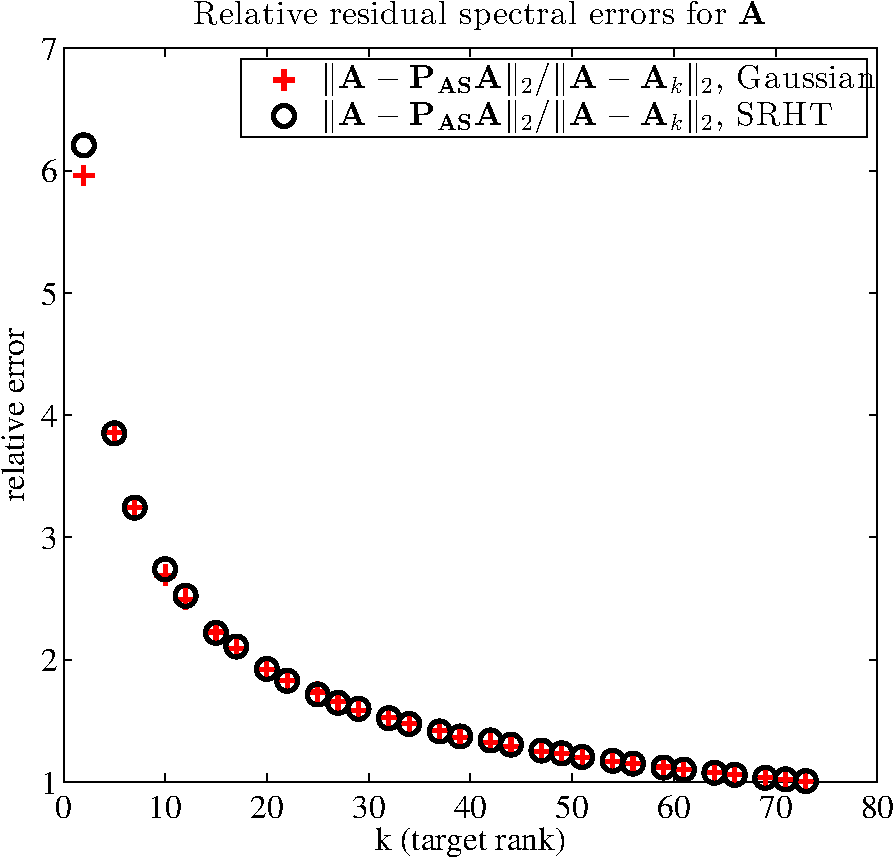
\includegraphics[width=2.2in, keepaspectratio=true]{experimentA-residual-spectral.pdf}%
%  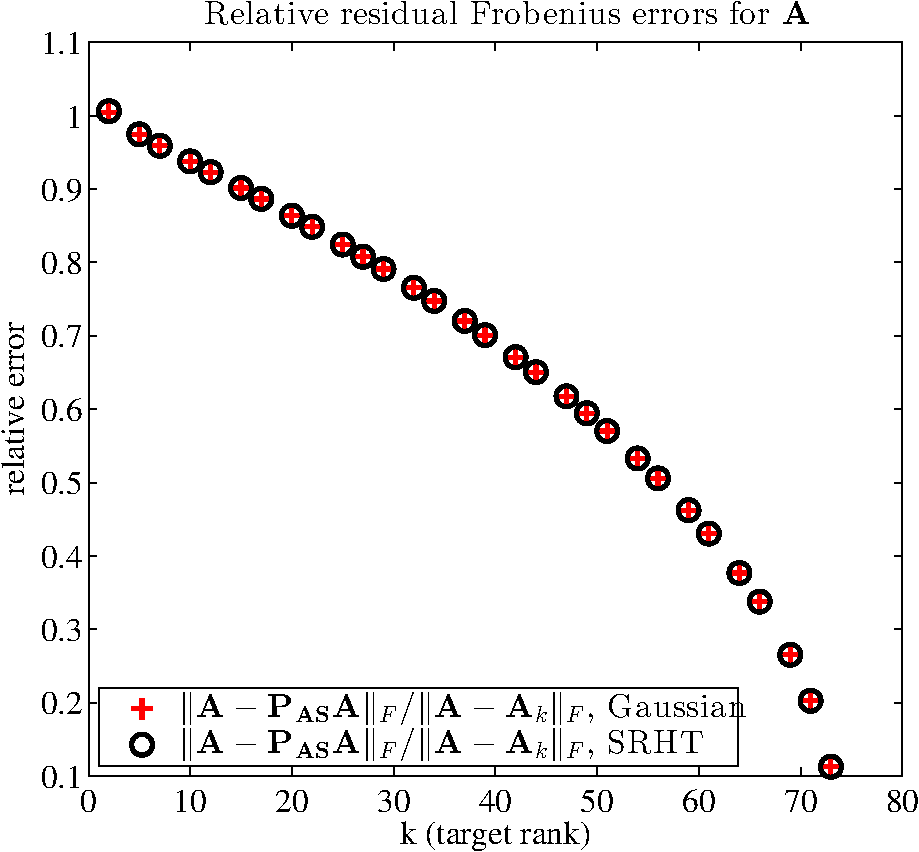
\includegraphics[width=2.2in, keepaspectratio=true]{experimentA-residual-frobenius.pdf}}
%  \vspace{1em}
%   Each point is the average of the errors observed over 30 trials,
%  where each approximation was constructed using $\ell = \lceil 2 k \log n \rceil.$
% \end{frame}
% 
% \begin{frame}
%   \centerline{%
%  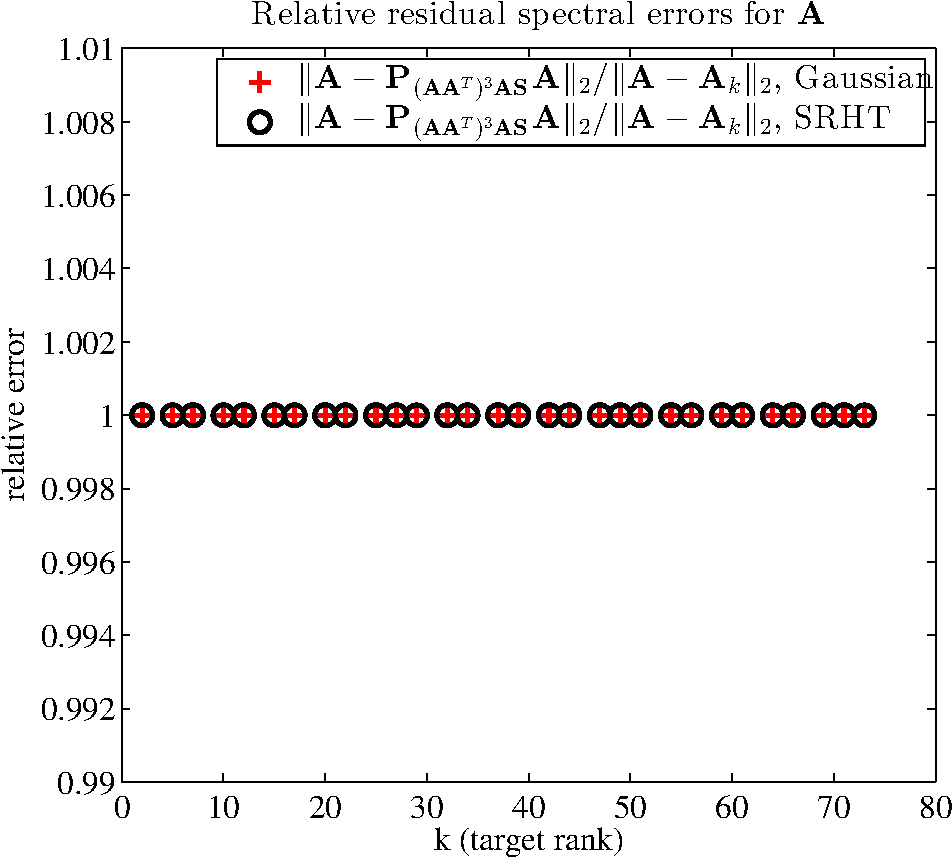
\includegraphics[width=2.2in, keepaspectratio=true]{experimentD-residual-spectral.pdf}%
%  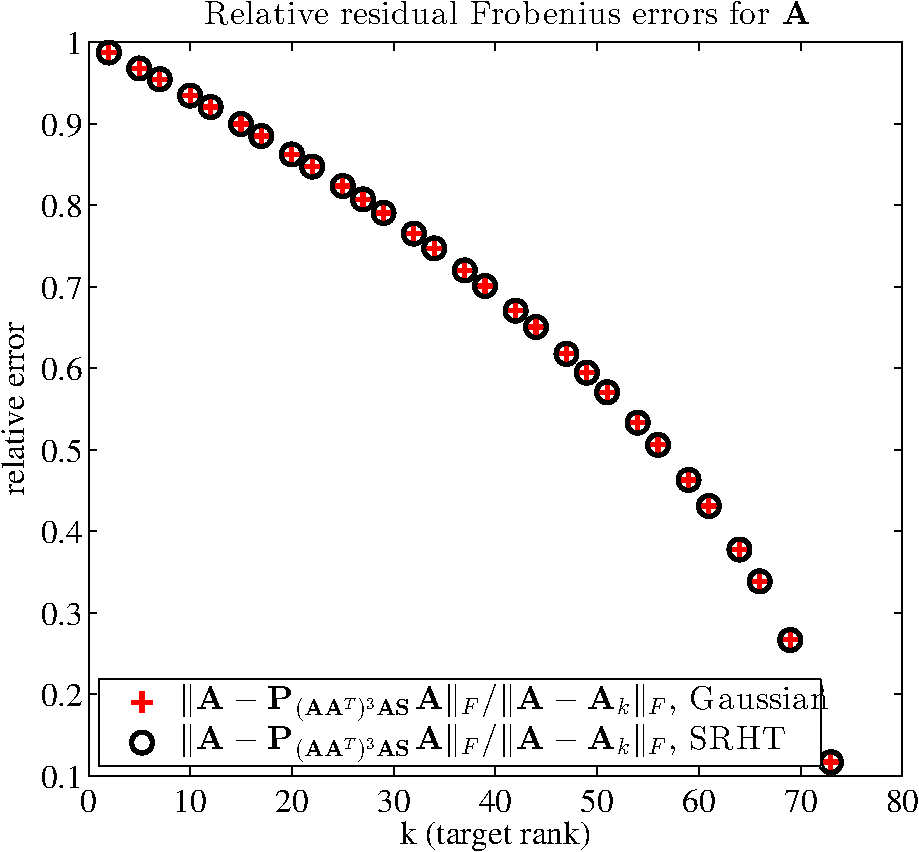
\includegraphics[width=2.2in, keepaspectratio=true]{experimentD-residual-frobenius.pdf}}
%  \vspace{1em}
%  We apply the power method with $p=3,$ while keeping $\ell = \lceil 2 k \log n \rceil.$
% \end{frame}
% 
% \begin{frame}
% 
%  Let $n = 1024;$ consider the diagonal matrix $\matB \in \R^{n \times n}$ with 
%  entries $(\matB)_{ii} = 100(1 - (i-1)/n).$
%  \[
%   \matB = \left[ 
%           \begin{matrix} 100 &  0     & 0 & \ldots \\
%                           0  & 99.902 & 0 & \ldots \\
%                           0  & 0      & \ddots & \ldots \\
%                           0  & \ldots & 0 & 0.098 
%           \end{matrix}
%           \right]
%  \]
% 
%   $\matB$ is full-rank, has slowly decaying spectrum, and only $k$ columns of $\matB$
%   provide any information on the dominant $k$-dimensional left singular space of $\matB.$
% \end{frame}
%  
% \begin{frame}
% \centerline{%
%  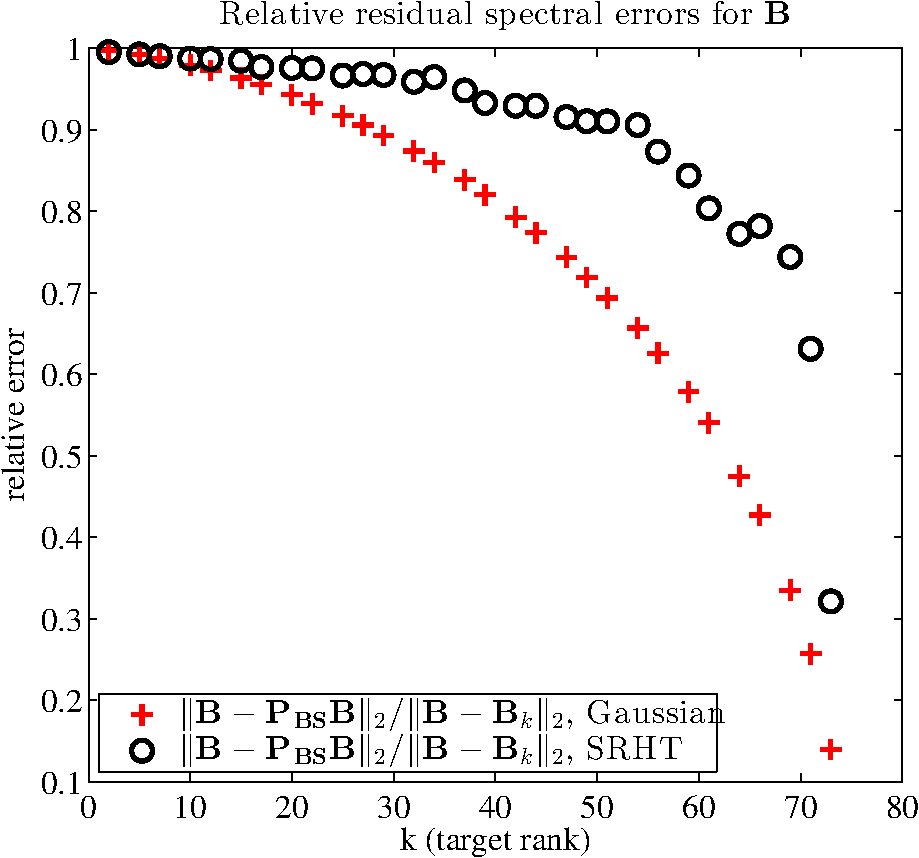
\includegraphics[width=2.2in, keepaspectratio=true]{experimentB-residual-spectral.pdf}%
%  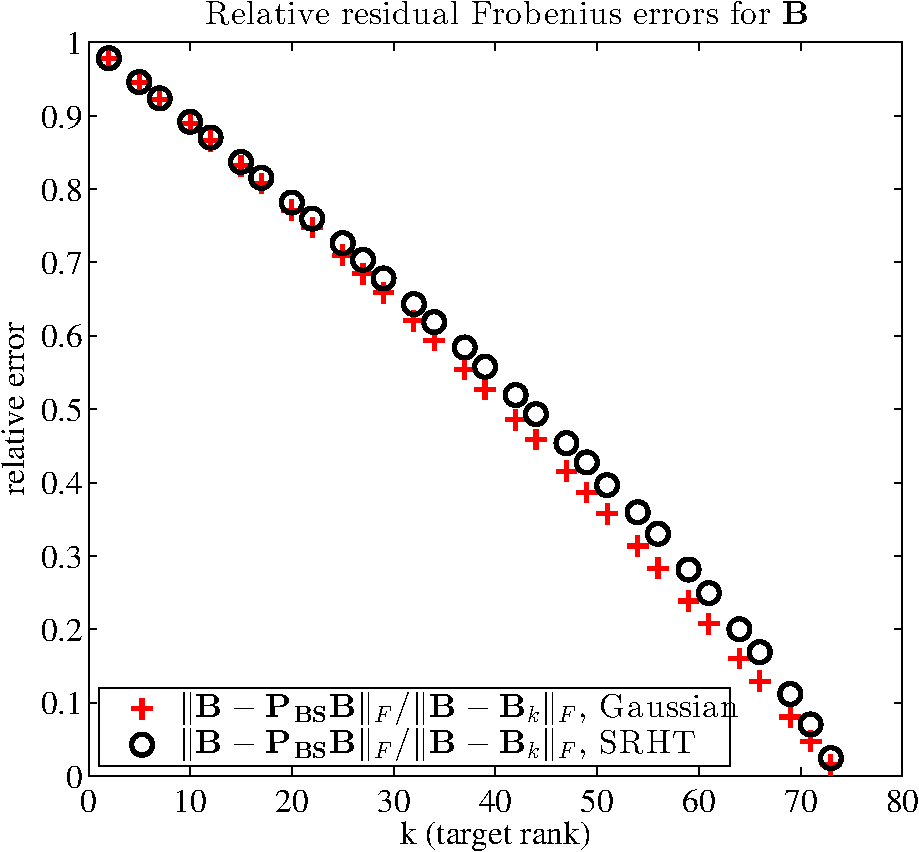
\includegraphics[width=2.2in, keepaspectratio=true]{experimentB-residual-frobenius.pdf}}
%  \vspace{1em}
%  Each point is the average of the errors observed over 30 trials,
%  where each approximation was constructed using $\ell = \lceil 2 k \log n \rceil.$
% \end{frame}
% 
% \begin{frame}
%   
%  Consider $\matC = \matU \matB \matV\transp,$ where $\matU$ and $\matV$
%  are obtained by taking the SVD of an $n \times n$ matrix of i.i.d. $\mathcal{N}(0,1)$ random variables,
%  $\matG = \matU \matSig \matV\transp.$
%  
% \[
%  \matC = \matU \left[ 
%           \begin{matrix} 100 &  0     & 0 & \ldots \\
%                           0  & 99.902 & 0 & \ldots \\
%                           0  & 0      & \ddots & \ldots \\
%                           0  & \ldots & 0 & 0.098 
%           \end{matrix}
%           \right] \matV\transp
% \]
% 
%  $\matC$ is also full-rank and has slowly decaying spectrum, but every column of $\matC$ contains
%  information on every singular space of $\matC.$
% \
% \end{frame}
% 
%  \begin{frame}
% \centerline{%
%  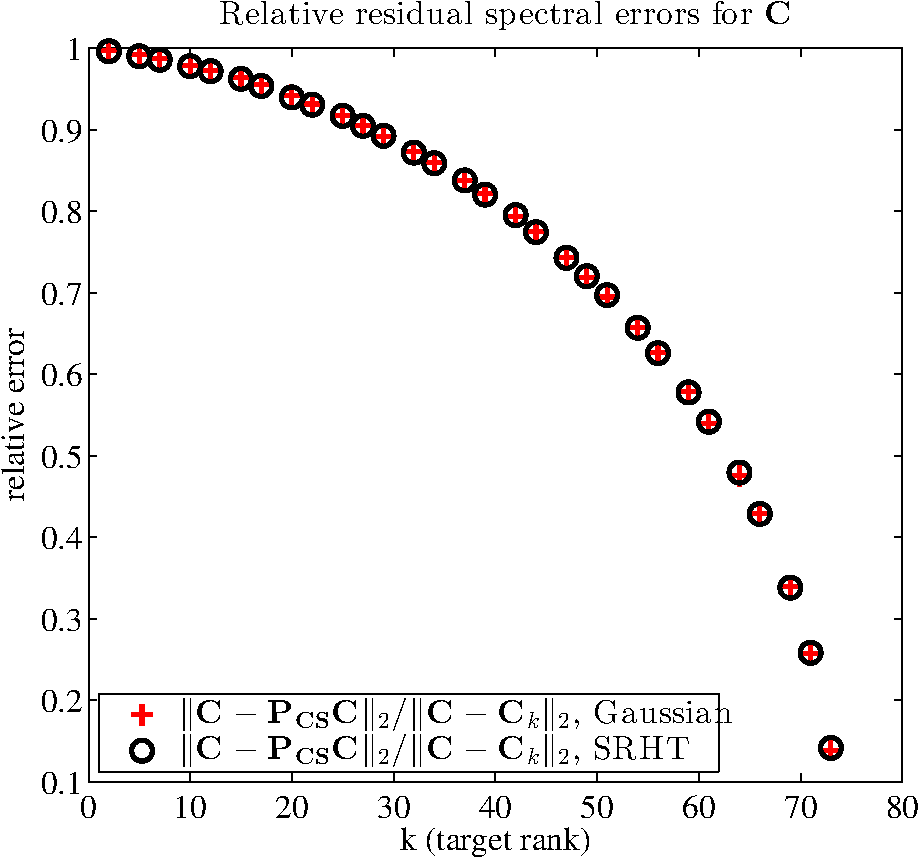
\includegraphics[width=2.2in, keepaspectratio=true]{experimentC-residual-spectral.pdf}%
%  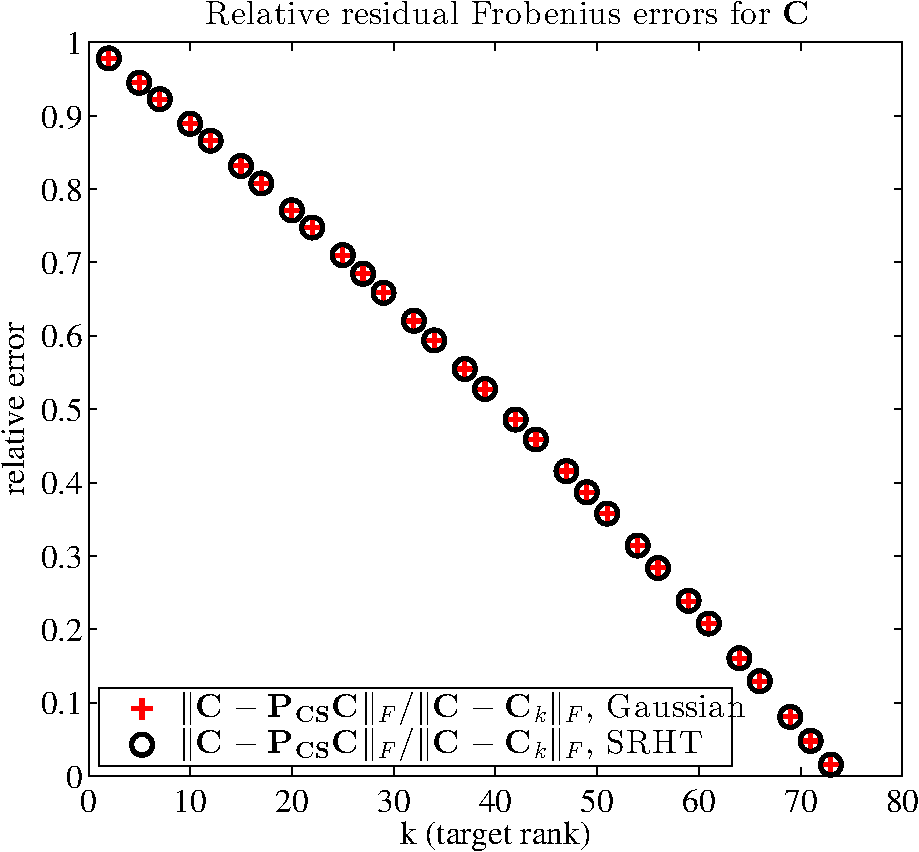
\includegraphics[width=2.2in, keepaspectratio=true]{experimentC-residual-frobenius.pdf}}
%  \vspace{1em}
%  Each point is the average of the errors observed over 30 trials,
%  where each approximation was constructed using $\ell = \lceil 2 k \log n \rceil.$
%  \end{frame}
% 
%  \begin{frame}
%   Observations:
%   \begin{enumerate}
%    \item When $\matA$ is approximately low-rank, the SRHT and Gaussian low-rank approximations exhibit
%    about the same accuracy.
%    \item When $\matA$ is full rank the structures of the singular spaces are important. 
%    \begin{itemize} 
%    \item If the singular
%    vectors are ``flat'', then SRHT and Gaussian approximations have comparable accuracy. 
%    \item If the singular
%    vectors are axis-aligned, then Gaussian approximations outperform SRHT approximations.
%    \end{itemize}
%    \item Empirically, $\ell = \Omega(k \log n)$ seems to ensure SRHT approximations achieve relative-error bounds.
%   \end{enumerate}
% 
%  \end{frame}
%  
%  \begin{frame}{Prior work}
% 
%  Similar randomized structured projection schemes:
%  \begin{itemize}
%   \item \refer{Woolfe et al. 2008}: if $\ell = \const{O}(k^2),$ then 
%    \[
%      \|\matA - \tilde{\matA}\|_2 \leq \sqrt{\max\{m,n\}} \|\matA - \matA_k\|_2
%    \]
%   \item \refer{Nguyen et al. 2009}: if $\ell = \const{O}(\varepsilon^{-1} k \log k),$ then
%   \begin{align*}
%    \|\matA - \tilde{\matA}\|_2 & \leq (2 + \sqrt{n/\ell}) \|\matA - \matA_k\|_2 \\
%    \|\matA - \tilde{\matA}\|_\rf & \leq (1 + \epsilon) \|\matA - \matA_k\|_\rf
%   \end{align*}
%  \end{itemize}
% 
%  Exactly the same SRHT scheme:
%  \begin{itemize}
%   \item \refer{Halko et al. 2011}: if $\ell = \const{O}(k \log k),$ then for $\xi \in \{2, \rf\},$
%   \[ \|\matA - \matP_{\matA \matS}\|_\xi \leq (1 + \sqrt{n/\ell})\|\matA - \matA_k\|_\xi.
%   \]
%  \end{itemize}
% 
% \end{frame}
% % 
% \begin{frame}{For comparison}
%  
%  It follows from \refer{Halko et al. 2011} that when $\matS$ is Gaussian and 
%  $\ell = \Omega(\epsilon^{-2} k \log n),$
%  \begin{align*}
%   \|\matA - \matP_{\matA\matS} \matA\|_2 & \leq \left(1 + \frac{\epsilon}{\sqrt{\log n}}\right) \|\matA - \matA_k\|_2
%     + \frac{\epsilon}{\sqrt{k \log n}} \|\matA - \matA_k\|_\rf \\
%   \|\matA - \matP_{\matA\matS} \matA\|_F & \leq \left(1 + \frac{\epsilon}{\sqrt{\log n}}\right) \|\matA - \matA_k\|_F
%    % + \frac{\epsilon}{\sqrt{k}} \|\matA - \matA_k\|_2
%  \end{align*}
%  simultaneously with probability at least $1 - \frac{2}{n}.$
%  \vspace{1em}
%  
%  Gaussians and SRHTs behave quite similar empirically, yet prior analyses for SRHTs are qualitatively poorer than this analysis.
% \end{frame}
% 
% \begin{frame}{Improved Error Bounds}
%  \begin{block}{\refer{Boutsidis and G. 2012}}
%   If $k = \Omega(\log n)$ and $\ell = \Omega( \epsilon^{-2} k \log n ),$ then
%   \begin{align*}
%       \|\matA - \matP_{\matA\matS} \matA\|_2 & \leq 
%        (4 + \epsilon )\cdot \|\matA - \matA_k\|_2 + \frac{\epsilon}{\sqrt{k}} \|\matA - \matA_k\|_\rf \\
%    \|\matA - \matP_{\matA\matS} \matA\|_\rf & \leq (1 + 11\epsilon^2) \|\matA - \matA_k\|_\rf
%   \end{align*}
%   simultaneously with probability at least $1 - \delta.$
%  \end{block}
% 
%  This result essentially holds when $\matS$ is any subsampled orthogonal transformation,
%  \[
%   \matS = \sqrt{\frac{n}{\ell}} \matD \matT \matR,
%  \]
%  where $\matT$ is an orthogonal transformation matrix with entries on the order of $n^{-1/2}.$
% \end{frame}
% 
% \begin{frame}{Notation}
% \begin{itemize}
%  \item Partition the SVD of $\matA:$
% \vspace{-1em}
%  \[ 
% \mat{A} = \mat{U} \matSig \mat{V}\transp = \bbordermatrix{%
% &^k \vspace{-0.75ex} & \!\!^{n-k}  \hspace{1ex}\cr
% & \vspace{0.25ex} \mat{U}_1 \hspace{-2ex} & \mat{U}_2 
% }
% \bbordermatrix{%
% & \vspace{-0.75ex} ^k &\!\!^{n-k} \hspace{1ex}\cr
% & \matSig_1 & \cr
% & \vspace{0.5ex} & \matSig_2 
% }
% \left[
% \begin{matrix}
% \mat{V}_1\transp \\
% \mat{V}_2\transp  
% \end{matrix}
% \right].
% \]
%  Note that $\matA_k = \matU_1 \matSig_1 \matV_1\transp.$ 
% 
%  \item Define
% \[
%  \matOmega_1 = \matV_1\transp \matS \quad \text{ and } \matOmega_2 = \matV_2\transp \matS,
% \]
% to capture the interaction of $\matS$ with the dominant and residual right singular spaces of $\matA.$
% \vspace{1em}
% \end{itemize}
% 
% \end{frame}

% \begin{frame}{Key tools}
% 
% \begin{itemize}
% 
%  \item Matrix Chernoff inequalities that show that if the energy of $\matM$ (i.e. its Frobenius norm) is evenly distributed throughout its columns, then
%  matrices consisting of randomly sampled columns of $\matM$ have similar extreme singular values to $\matM.$
%  
%  \item An extension of a result in \refer{Tropp 2011} to show right multiplication by $\matD\matH$ distributes the energy of any matrix
%  $\matM$ evenly over its columns.
% \end{itemize}
% 
%  
% \end{frame}
% 
% \begin{frame}{Sketch of spectral norm proof}
%  \begin{enumerate}
%   \item By the structural result,
%  \[
%   \|\matA - \matP_{\matA\matS} \matA\|_2^2 \leq \|\matA - \matA_k\|_2^2 + \|\matSig_2 \matV_2\transp \matD \matH \matR \|_2^2 
%                                                 \cdot \bigbar (\matV_1\transp \matD \matH \matR)^\pinv\bigbar_2^2.
%  \]
%  \item
%  $\matD \matH$ spreads the energy of $\matV_1\transp$ throughout its columns sufficiently that when enough columns are
%  selected by $\matR$, the spectrum of the resulting matrix is close to that of $\matV_1\transp.$ Consequently,
%  \[
%   \|\matA - \matP_{\matA\matS} \matA\|_2^2 \leq \|\matA - \matA_k\|_2^2 + (1 - \sqrt{\epsilon})^{-1} \|\matSig_2 \matV_2\transp \matD \matH \matR \|_2^2.       
%  \]
%  \end{enumerate}
% \end{frame}
% 
% \begin{frame}
%  \begin{enumerate}
%  \setcounter{enumi}{2}
%   \item $\matD\matH$ spreads the energy of $\matSig_2 \matV_2\transp$ throughout its columns sufficiently that when enough columns
%   are selected by $\matR,$ the norm of the resulting matrix is not much larger than that of $\matSig_2:$
%   \begin{multline*}
%   \mathbb{P}\left\{\|\matSig_2 \matV_2\transp \matD \matH \matR\|_2^2 \leq 
%     \left(5 + \frac{\log(n/\delta)}{\ell} \right) \|\matSig_2\|_2^2 + \right. \\
%     \left. \quad \quad \const{O}\left(\frac{\log(n/\delta)^{3/2}}{\ell}\right) \|\matSig_2\|_F^2 \right\} \geq 1 - \delta.
%   \end{multline*}
%   
%   \item Combine these pieces and use our lower bounds on $k$ and $\ell$ to simplify:
%   \[ 
%    \|\matA - \matP_{\matA\matS} \matA\|_2 \leq (4 + \epsilon) \|\matA - \matA_k\|_2 + \frac{\epsilon}{\sqrt{k}}\|\matA - \matA_k\|_\rf.
%   \]
% 
%  \end{enumerate}
% 
% \end{frame}
% 
% \begin{frame}{Proof sketch}
% \begin{itemize}
%  \item Bounding $\bigbar \matSig_2 \matOmega_2 \matOmega_1^\pinv\bigbar_2^2$ and $\bigbar \matSig_2 \matOmega_2 \matOmega_1^\pinv\bigbar_\rf^2$
%  reduces to showing that the columns of $\matM \matD \matH$ all have roughly the same norm when $\matM$ is an arbitrary matrix:
%  \[
%   \max_{j=1,\ldots,n} \|(\matM \matD \matH)_{j}\|_2 \leq \frac{\|\matM\|_\rf}{\sqrt{n}} + \frac{t\|\matM\|_2}{\sqrt{n}} 
%  \]
% with high probability. 
%  \item \refer{Tropp 2011} shows this is true when
% $\matM$ has orthonormal rows. The result for arbitrary $\matM$ is a generalization of this argument.
% 
% \end{itemize}
% \end{frame}

\begin{frame}{Nystr\"om extensions}
 The simplest SPSD sketch is the Nystr\"om extension:
 \[ 
  \matA = \matC \matW^\pinv \matC\transp,
 \]
 where $\matC$ consists of uniformly randomly chosen columns of $\matA$ and $\matW$ consists of 
 $\matC$ restricted to the corresponding rows.
 \centerline{\includegraphics[width=4in,keepaspectratio=true]{figures/spsd/nystrom-procedure}}
\end{frame}

\begin{frame}
Nystr\"om extensions perform well when 
the information in its top $k$-dimensional eigenspace is spread throughout $\mat{A}:$

\[
 \mat{A} = 20 \left[\begin{matrix} 1 \\ 0 \\ 0 \\ 0 \end{matrix}\right]
              \left[\begin{matrix} 1 & 0 & 0 & 0 \end{matrix}\right] = \left[\begin{matrix}
  20 & 0 & 0 & 0 \\
  0    & 0 & 0 & 0 \\
  0    & 0 & 0 & 0 \\
  0    & 0 & 0 & 0
 \end{matrix}
 \right]
\]
versus
\[
\mat{A} = 20 \left[\begin{matrix} 1/2 \\ -1/2 \\ -1/2 \\ 1/2 \end{matrix}\right]
              \left[\begin{matrix} 1/2 & -1/2 & -1/2 & 1/2 \end{matrix}\right] =              
  \left[\begin{matrix}
                 5 & -5 & -5 & -5 \\
                 -5 & 5 & 5 & -5 \\
                 -5 & 5 & 5 & -5 \\
                  5 & -5 & -5 & 5
                \end{matrix}
  \right]
 \]
 
 \textbf{key point}: we need the support of the top $k$ eigenvectors to be spread out.
 \end{frame}
 
 \begin{frame}

 Let $\matU_1$ be an orthonormal basis for the dominant $k$-dimensional eigenspace of $\matA.$
 \vspace{0.7em}
 
 A measure of the 
 ``spreadness'' of the eigenvectors in $\matU_1$ is given by the \emph{coherence} of $\matU_1:$
 
 \[
  \mu := \frac{n}{k} \max\nolimits_j \|(\matU_1)_j\|_2^2.
 \]
 
 \begin{itemize}
  \item $\mu$ is between $1$ (best case) and $n/k$ (worst case)
  \item $\mu$ both theoretically \emph{and empirically} determines the feasibility of Nystr\"om extensions...
 \end{itemize}

 \end{frame}
 
  \begin{frame}
  
 \begin{figure}[h]
 \centering
 \centerline{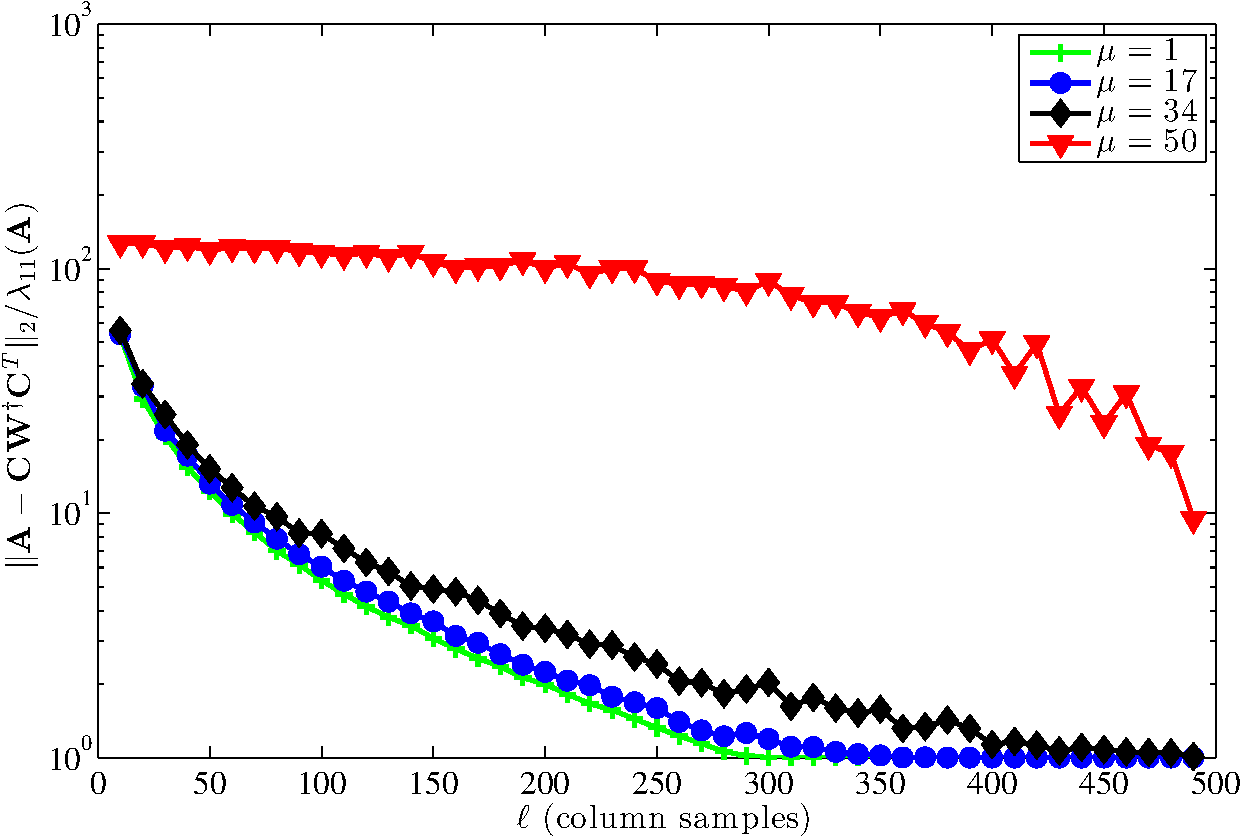
\includegraphics[width=4in,keepaspectratio=true]{figures/spsd/nystromcoherencedependence}} 
 \end{figure}
 \vspace{-2em}
$\matA \in \R^{500 \times 500}$ is full-rank, but numerically rank 20. The target rank $k = 10.$
Each point is the average of 60 trials.

\end{frame}

\begin{frame}
  The best previous error bound on the error of Nystr\"om extensions in terms of the coherence is 
  
  \begin{block}{\refer{Talwalkar and Rostamizadeh 2010}}
   Let $\mat{A}$ be exactly rank-$k$. If $\ell = \Omega(\mu k \log(k/\delta)),$ then 
   \[ \|\mat{A} - \mat{C} \mat{W}^\pinv \mat{C}\transp\| = 0 \]
   with probability at least $1-\delta.$
  \end{block}
 
  What about $\matA$ that are not exactly low-rank?
  \end{frame}
  
\begin{frame}{Optimal bounds for Nystrom extensions}
  The approximation errors can be bounded when $\ell$ is proportional to the coherence; our framework
  gives the following result.
  
  \begin{block}{Spectral-norm error bound \refer{G. 2011}}
   If $\ell \geq 8 \mu k \log(k/\delta),$ then
   \[ \|\mat{A} - \mat{C} \mat{W}^\pinv \mat{C}\transp\|_2 \leq \|\matA - \matA_k\|_2 \left(1 + \frac{2 n}{\ell} \right)\]
   with probability at least $1 - \delta.$ 
   %and
  % \[ \|\mat{A} - \mat{C} \mat{W}^\pinv \mat{C}\transp\|_2 \leq \|\matA - \matA_k\|_2 +
  %  \left( \frac{2}{\delta^2} \tr((\matA - \matA_k)^{2p-1}) \right)^{1/(2p-1)}\]
  % with probability at least $1 - 2\delta.$
  \end{block}

  A matrix constructed in \refer{Boutsidis et al. 2011} shows that this bound is \textbf{tight}: there are matrices for which the relative
  spectral-norm error is on the order of $n/\ell.$
 \end{frame} 

 
 \begin{frame}{SPSD Sketches}
 
 SPSD sketches generalize the Nystr\"om extension, by potentially mixing information across the columns of $\matA,$ 
 thereby removing the sensitivity to $\mu.$
 \vspace{0.7em}
 
 Fix an arbitrary ``sketching matrix'' $\mat{S} \in \R^{n \times \ell}.$ The corresponding sketch of the SPSD matrix $\matA \in \R^{n \times n}$
 is
  \[
   \hat{\mat{A}} = \mat{C} \mat{W}^\pinv \mat{C}\transp,
  \]
  where $\mat{C} = \mat{A}\mat{S}$ and $\mat{W} = \mat{S}\transp \mat{A} \mat{S}.$
  
  \begin{itemize}
   \item The sketch $\hat{\mat{A}}$ is also SPSD.
   \item This model allows for both column-sampling based approximations (e.g. Nystr\"om extensions) and column-mixture
  based approximations. 
   \item To form the sketch requires only one pass over $\matA.$
  \end{itemize}
  
\end{frame}
 
\begin{frame}{Choice of sketching matrices}

Dominant arithmetic cost of forming the sketch is the matrix--matrix multiply $\matA\matS.$
\vspace{1em}

A natural choice for $\matS$ is a matrix of i.i.d. $\mathcal{N}(0,1)$ Gaussians, proposed in \refer{Martinsson et al. 2006}. 
\begin{itemize}
 \item Computation of 
$\matA \matS$ takes $\const{O}(n^2\ell)$ time for general $\matA$.
 \item The columns of $\matA$ are well-mixed.
\end{itemize}

\vspace{1em}

\refer{Woolfe et al. 2008} proposed using \emph{structured} random projections.

\begin{itemize}
 \item Computation of $\matA \matS$ takes reduced time $\const{O}(n^2 \log(\ell)).$
 \item Mixing not as uniform, so potential accuracy loss.
\end{itemize}

\end{frame}

% \begin{frame}
%  Subsampled randomized orthogonal transforms are one class of structured random projections:
%  \[
%   \matS = \sqrt{\frac{n}{\ell}} \matD \matT \matR \in \R^{n \times \ell}.
%  \]
% Here:
% \begin{itemize}
%  \item  $\matD$ is a diagonal matrix of random signs,
%  \item  $\matR$ selects $\ell$ columns at random, and 
%  \item $\matT$ is the matrix of an orthogonal transformation that is associated with a fast transform.
% \end{itemize}
% 
% Examples: if $\matT$ is the real Fourier transformation or $\matT$ is the normalized Walsh--Hadamard matrix, then
% the matrix--matrix product $\matA \matS$ can be computed in time $\mathrm{O}(n^2\log\ell).$
% 
% % = n^{-1/2} \matH_n \in \R^{n \times n}$ is the normalized Walsh--Hadamard matrix. The matrices $\matH_n$ are
% % defined recursively by
% % \[
% %  \matH_n = \left[
% % \begin{array}{cc}
% %   \matH_{n/2} &  \matH_{n/2} \\
% %   \matH_{n/2} & -\matH_{n/2}
% % \end{array}\right],
% % %
% % \qquad \mbox{with} \qquad
% % %
% % \matH_2 = \left[
% % \begin{array}{cc}
% %   +1 & +1 \\
% %   +1 & -1
% % \end{array}\right].
% % \]
% % \end{itemize}
% 
% 
% \end{frame}


\begin{frame}

We consider the following specific sketches, corresponding to different distributions on $\matS$:
 \begin{itemize}
  \item When $\matS$ selects columns uniformly at random without replacement from $\matA,$ 
   we call $\hat{\matA}$ a \textcolor{dgreen}{Nystr\"om extension}.
  \item When $\matS$ selects columns from $\matA$ randomly with replacement with probabilities proportional to their 
   \emph{leverage scores}, $\hat{\matA}$ is a \textcolor{dgreen}{leverage sketch}.
  \item When $\matS$ consists of i.i.d. $\mathcal{N}(0,1)$ Gaussians, $\hat{\matA}$ is a \textcolor{dgreen}{Gaussian sketch}.
  \item When $\matS$ is a subsampled randomized Fourier transform (SRFT), $\hat{\matA}$ is an \textcolor{dgreen}{SRFT sketch}.
 \end{itemize}

 \end{frame}

%  \begin{frame}
%  
%  The quality of the approximation depends on how well the range of the dominant $k$-dimensional left
%  singular space of $\matA$ is approximated by the range of $\matY.$
%  \vspace{.75em}
%  
%  We can use the ``power'' method to increase the accuracy of the approximation:
%  approximate $\matA$ with $\matP_{(\matA\matA\transp)^p \matA \matS} \matA:$
%  
%  \begin{enumerate}
%   \item Form $\matY = (\matA\matA\transp)^p \matA \matS.$
%   \item Take the QR decomposition $\matY = \matQ \matR.$
%   \item Form the low rank approximation $\matQ (\matQ\transp \matA).$
%  \end{enumerate}
% Requires only $2(p+1)$ passes over $\matA.$
% 
%  \vspace{.75em}
%  This methodology was popularized by \refer{Papadimitriou et al. 2000}, \refer{Sarl{\'o}s 2006}, and \refer{Martinsson et al. 2006}.
% \vspace{.75em}
% 
% Our design parameters: 
%   \begin{itemize}
%    \item $\ell,$ the number of samples ($k \leq \ell \ll \min\{m,n\}$) 
%    \item $\matS \in \R^{n \times \ell},$ the random sampling matrix.
%    \item $p,$ the number of iterations.
%   \end{itemize}
% \end{frame}
% 
% \begin{frame}
% Three factors determine probability of getting a good approximation:
% 
% \begin{itemize}
%  \item Spectral decay of $\matA$, e.g. the multiplicative gap $\sigma_{k+1}(\matA)/\sigma_k(\matA),$
%  or $(\sigma_{k+1}(\matA)/\sigma_k(\matA))^p.$
%  \item Type of randomness used to generate $\mat{S}.$
%  \vskip1em
%  \centerline{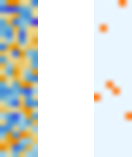
\includegraphics{samplingschemesillust}}
%  \vskip1em
%  \item Amount of oversampling (as $\ell \rightarrow n, \mat{P}_{\mat{A} \mat{S}} \mat{A} \rightarrow \mat{A}$).
% \end{itemize}
% 
% \end{frame}

% \begin{frame}{Nystr\"om extensions}
% 
% \begin{itemize}
%   \item Introduced in \refer{Williams and Seeger 2001} as a fast way
% of approximating the eigenvectors of large SPSD matrices arising in machine learning.
% 
%  \item Here $\matS$ selects $\ell$ columns uniformly at random from $\matA.$ 
%  
% \centerline{\includegraphics[width=4in,keepaspectratio=true]{nystrom-procedure}}
% 
%  \item It takes $\const{O}(\ell^3 + n \ell^2)$ operations to form this extension (for $p=1$).
% \end{itemize}
% 
% \end{frame}

% 
% \begin{frame}
%   Gaussian and SRFT sketches:
%  \begin{itemize}
%    \item SRFT sketching suggested in \refer{Chiu and Demanet 2012}
%    \item $\matS$ mixes the columns of $\matA$ together before sampling.
%    \item Mixing process ensures that no columns are ignored.
%    \item Gaussian sketches cost $\const{O}(\ell^3 + n^2 \ell)$ operations to form.
%    \item SRFT sketches cost $\const{O}(\ell^3 + n^2 \log \ell)$ operations to form.
%    
% \end{itemize}
%  
% \end{frame}
% 

\begin{frame}{Leverage scores}

Write the SVD of $\matA_k = \matU_1 \matSig_1 \matU_1\transp.$
The statistical leverage scores of the columns of $\mat{A}$ (with respect to rank $k$), are the scaled column norms
of $\matU_1\transp:$
\[
 \left\{ \ell_j := \frac{n}{k} \snorms{(\matU_1\transp)_j}, j=1,\ldots,n \right\}.
\]
\vfill
%\centerline{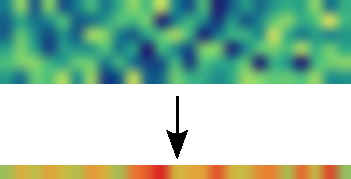
\includegraphics{levscoresillust}}
\centerline{
  \begin{overpic}{figures/spsd/levscoresillust}
 \put(-25,65){\fcolorbox{gray}{white}{$\matU_1\transp$}}
 \put(-29,0){\fcolorbox{gray}{white}{$\{\ell_j\}$}}
\end{overpic}
}
\vfill
Note that $\mu,$ the coherence, is the largest of the leverage scores of the columns of $\matA.$
\end{frame}

% \begin{frame}
% Leverage scores expose the dependence of the columns of $\mat{A}$ on $\matU_1.$ 
% \begin{itemize}
%  \item Let $\matA_j$ denote the $j$th column of $\matA$ and
% $\mat{u}_i$ denote the $i$th eigenvector, then
% \[
%  \mat{A}_j = \sum_{i=1}^{n} \lambda_i (\mat{u}_i \mat{u}_i^t)_j = \sum_{i=1}^k \lambda_i (\matU_1)_{ji} \mat{u}_i + \cdots
% \]
% so
% \[
%  \ell_j \propto \snorms{(\matU_1)_j} = \sum_{i=1}^k (\matU_1)_{ji}^2 
% \]
% is a measure of the influence $\matU_1$ has on $\mat{A}_j.$
%  \item We expect that columns with larger leverage scores provide more information on $\matU_1.$
% \end{itemize}
% 
% \end{frame}

\begin{frame}

Leverage sketches:
 \begin{itemize}
 \item The idea of leverage score sampling for forming column-sampling based low-rank approximations due to \refer{Drineas et al. 2008}.
  \item Columns are sampled randomly from $\matA$ with probability proportional to their leverage scores.
  \item Intuitively, leverage score sampling ensures that no important columns are ignored.
  \item {\color{red}{Assuming the leverage scores as given}}, costs $\const{O}(\ell^3 + n \ell^2)$ operations to form.
  \item The leverage scores can be approximated.
 \end{itemize}

\end{frame}

\begin{frame}{Empirical Performance (Exact schemes)}

  \centerline{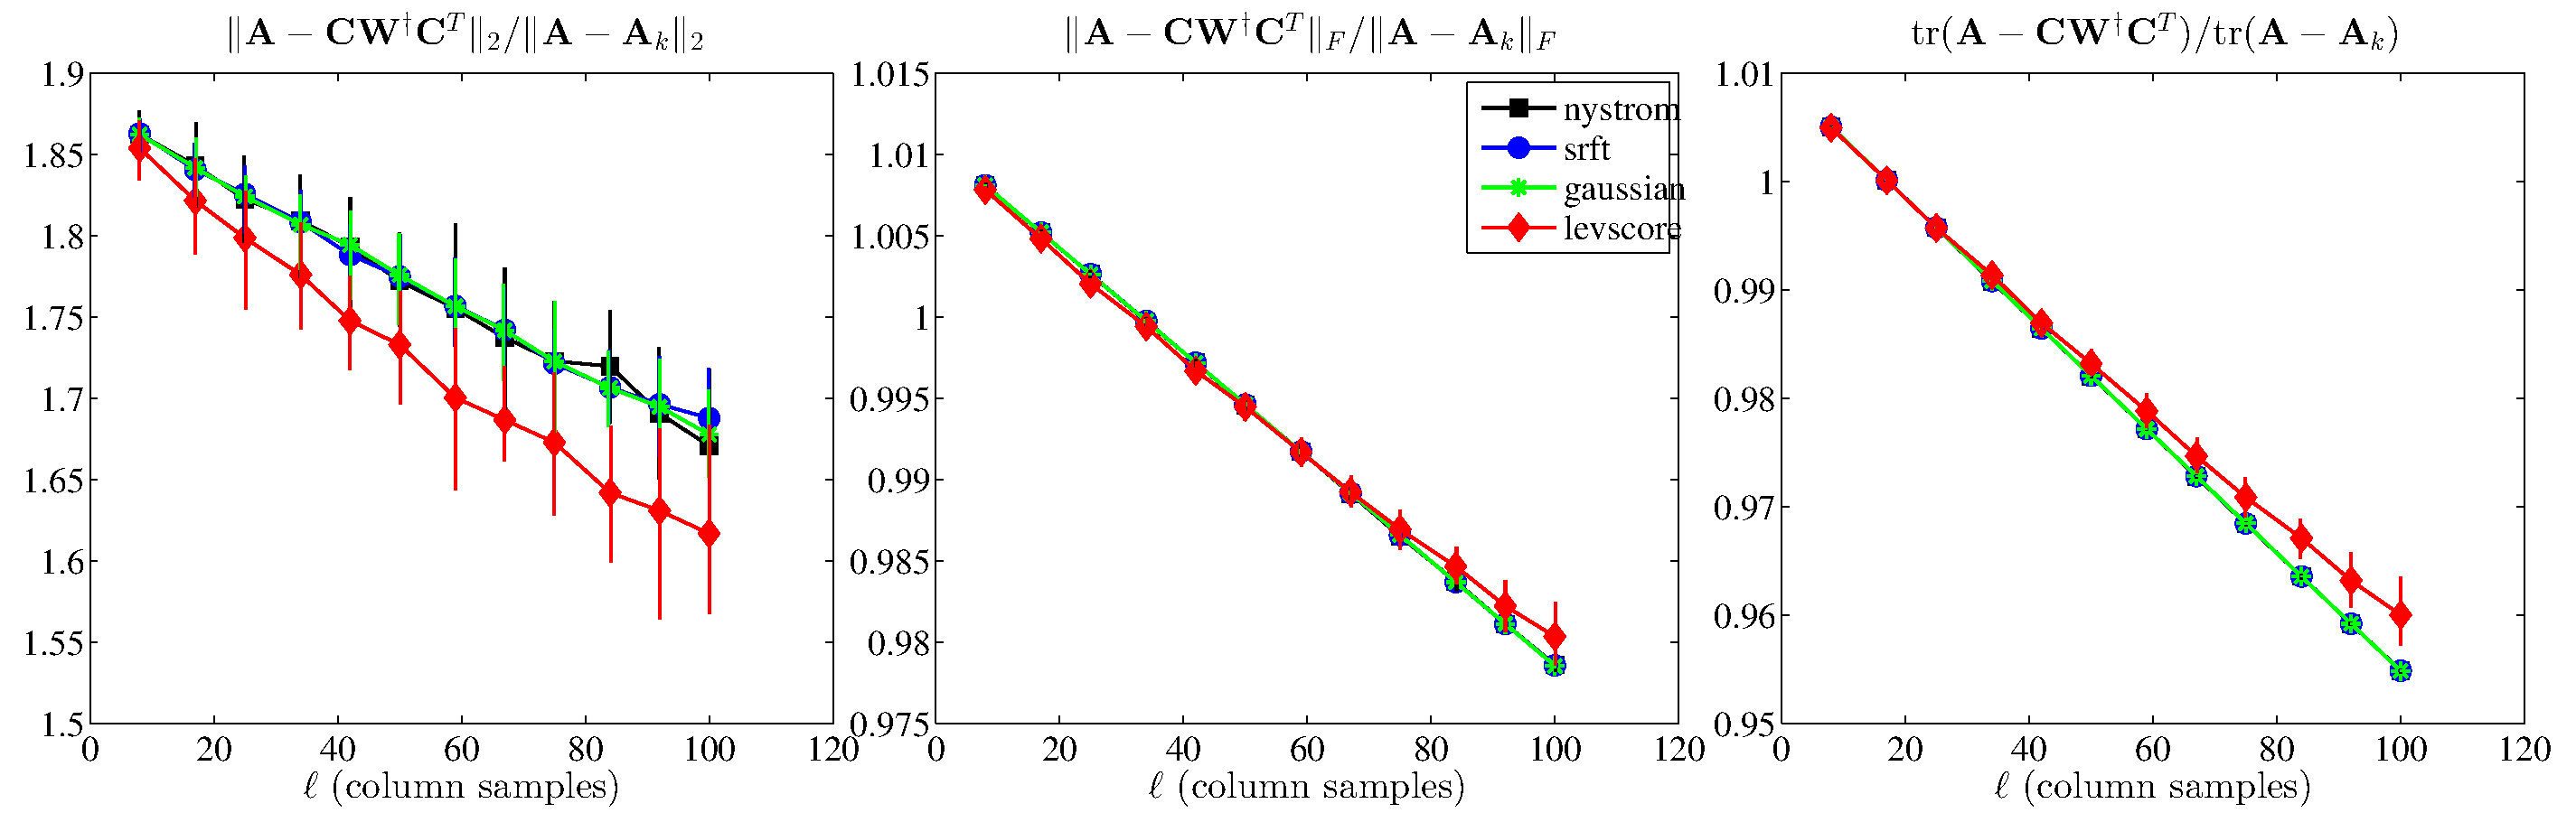
\includegraphics[width=4.7in, keepaspectratio=true]{figures/spsd/Dexterrank8exact-methods-nonfixed-rank-errors-range}}

 Dexter, a $2000 \times 2000$ Gram matrix from the UCI Machine Learning Repository. 
 Target rank $k= 8.$
\end{frame}

\begin{frame}

  \centerline{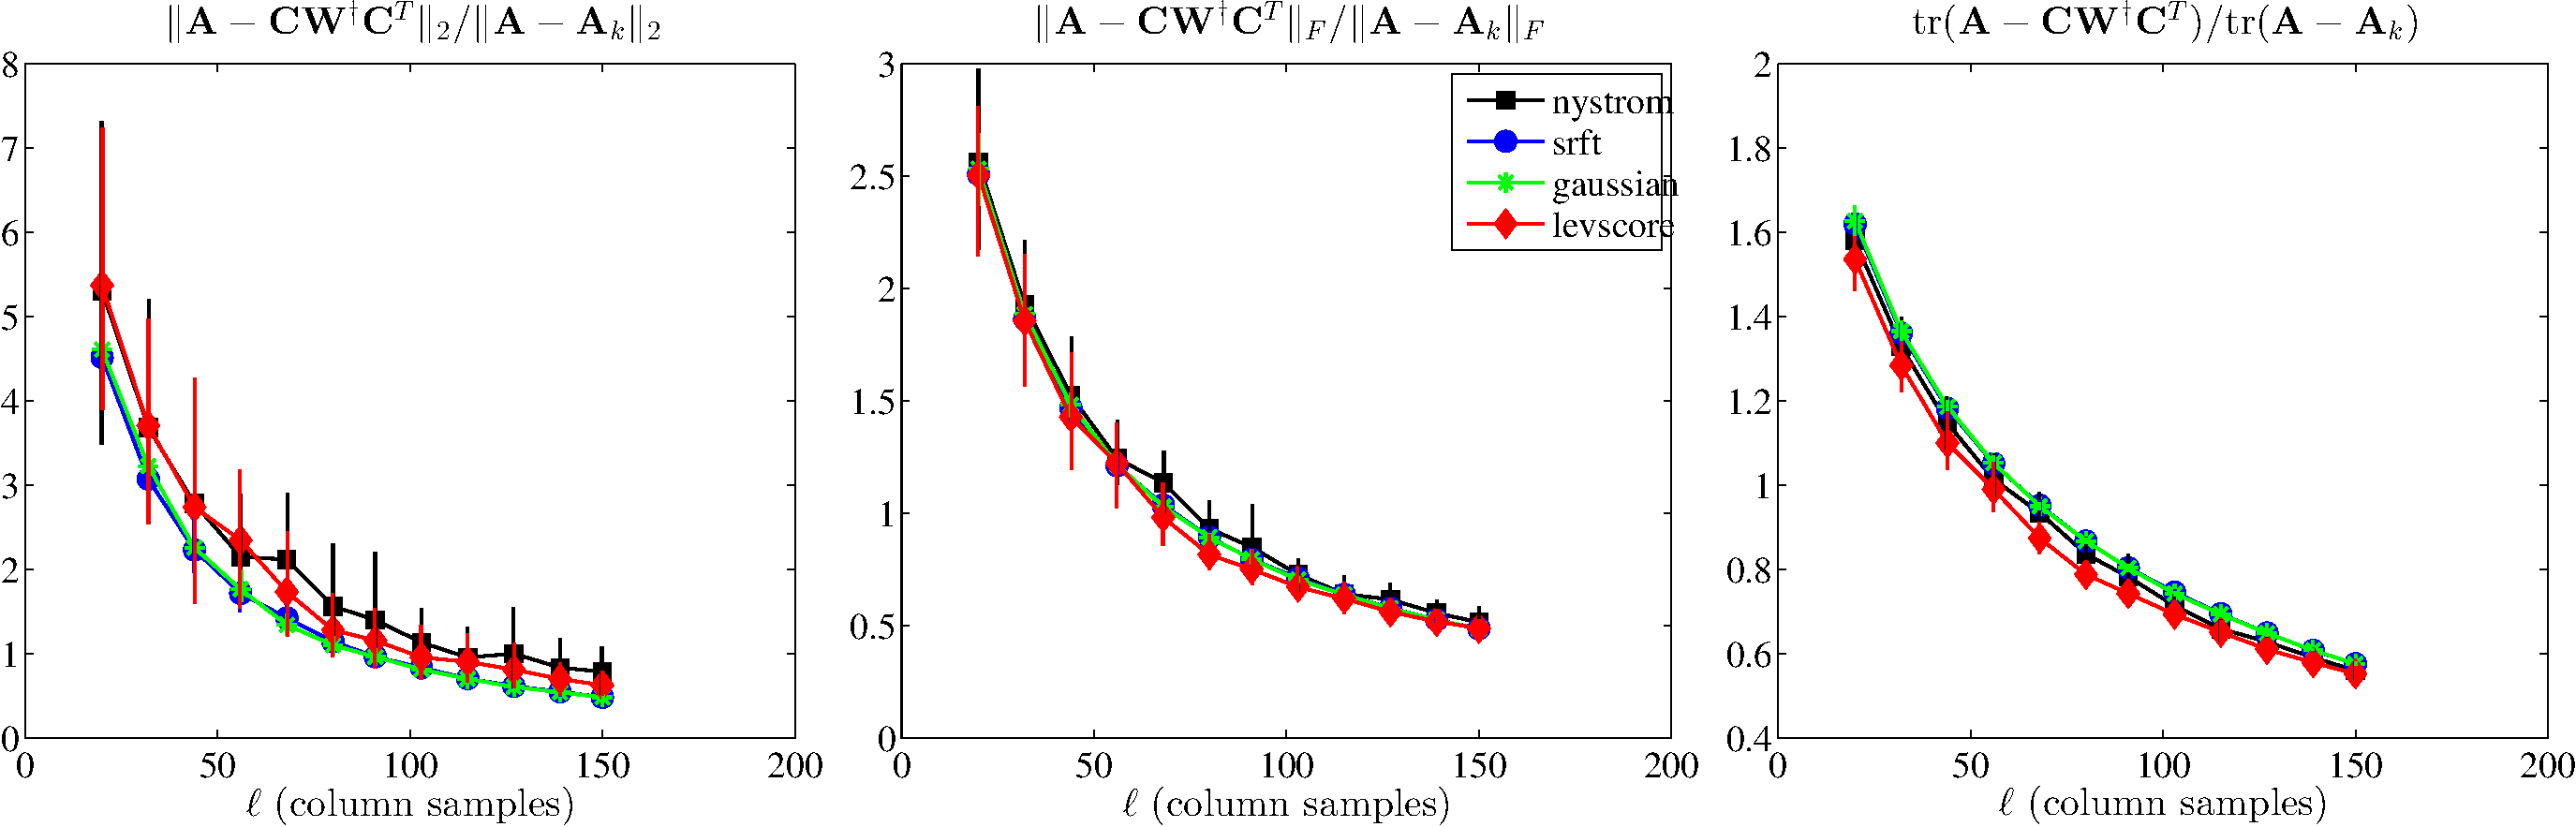
\includegraphics[width=4.7in, keepaspectratio=true]{figures/spsd/Abalonesigma1exact-methods-nonfixed-rank-errors-range}}

 Abalone, a $4898 \times 4898$ Radial Basis Kernel matrix from the UCI Machine Learning Repository. 
 Target rank $k= 20.$ 
\end{frame}

\begin{frame}
 
  \centerline{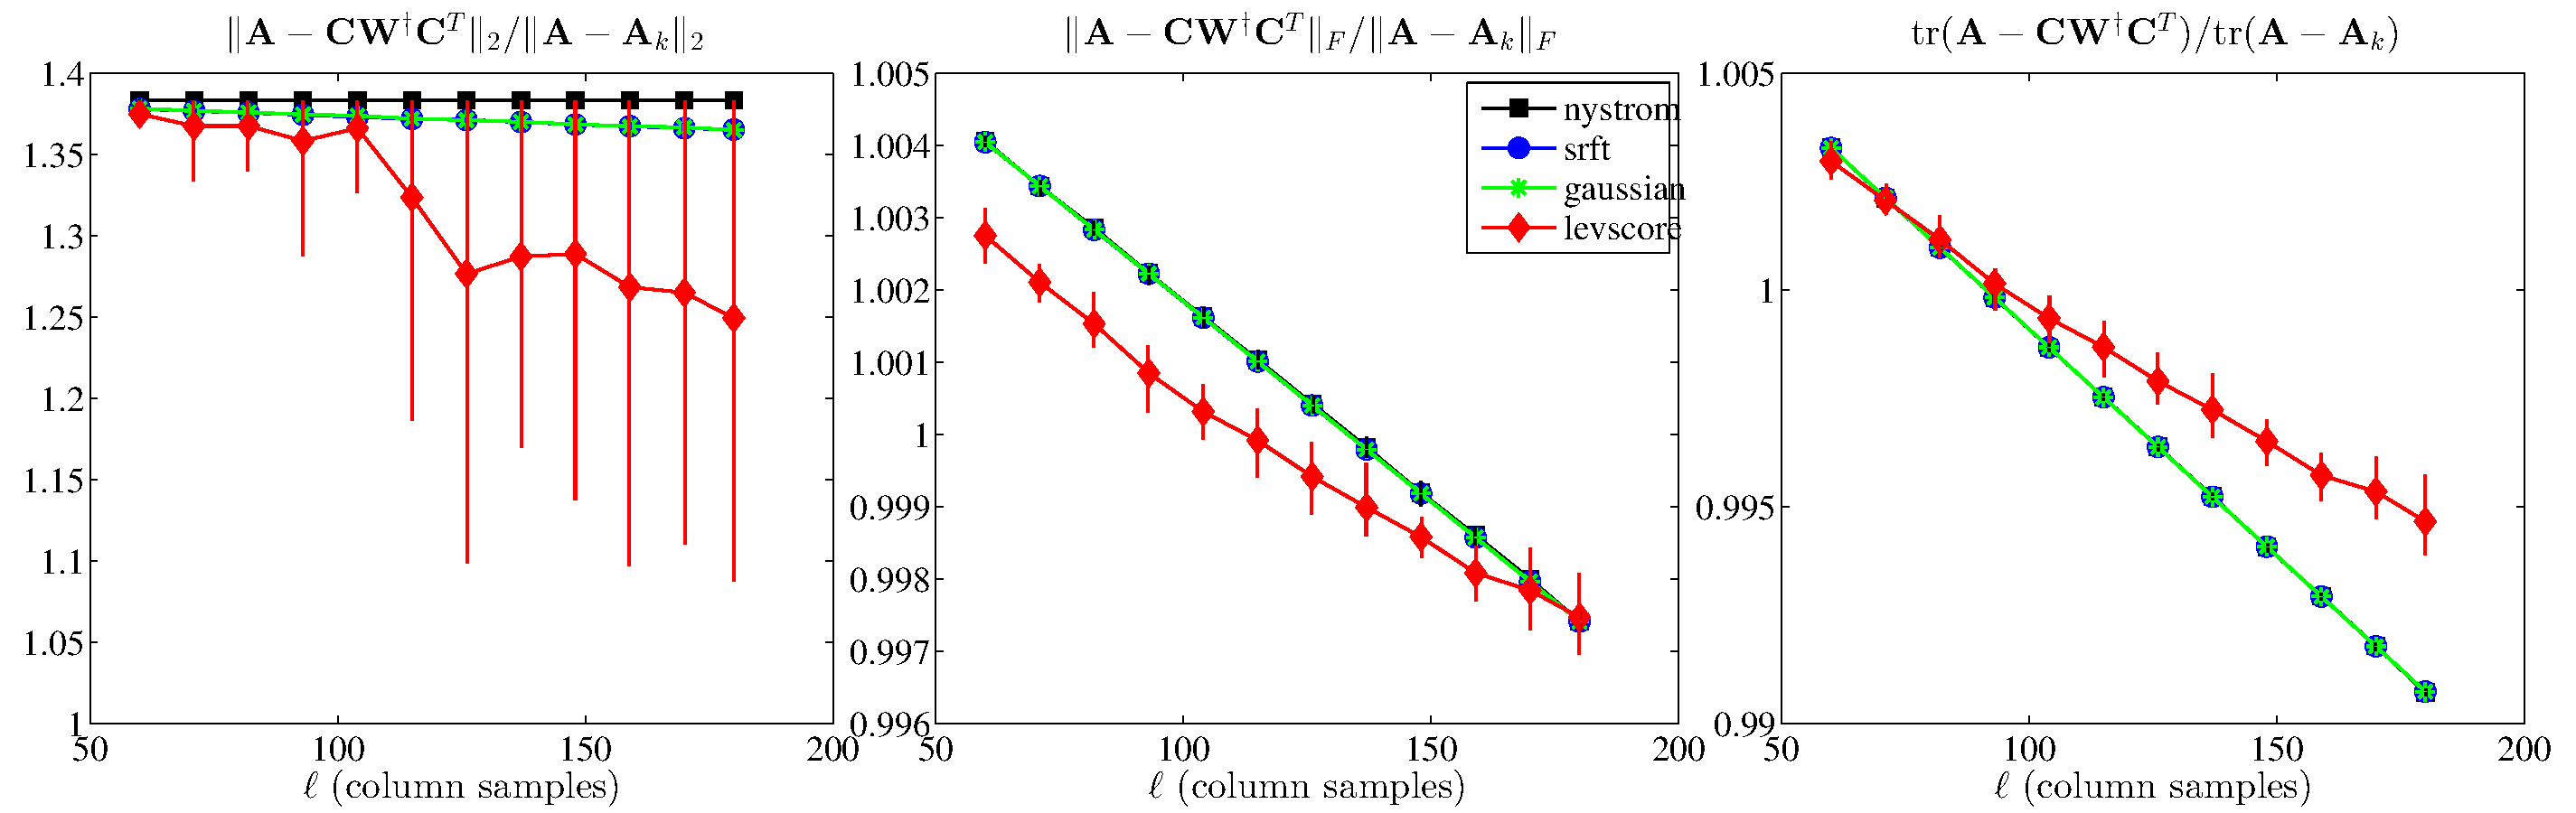
\includegraphics[width=4.5in, keepaspectratio=true]{figures/spsd/Enronrank60exact-methods-nonfixed-rank-errors-range}}
 Enron, a $10K \times 10K$ Graph Laplacian matrix from the Stanford SNAP collection. Target
 rank $k = 60.$ 
\end{frame}
% 
% 
% \begin{frame}
%  \centerline{%
%    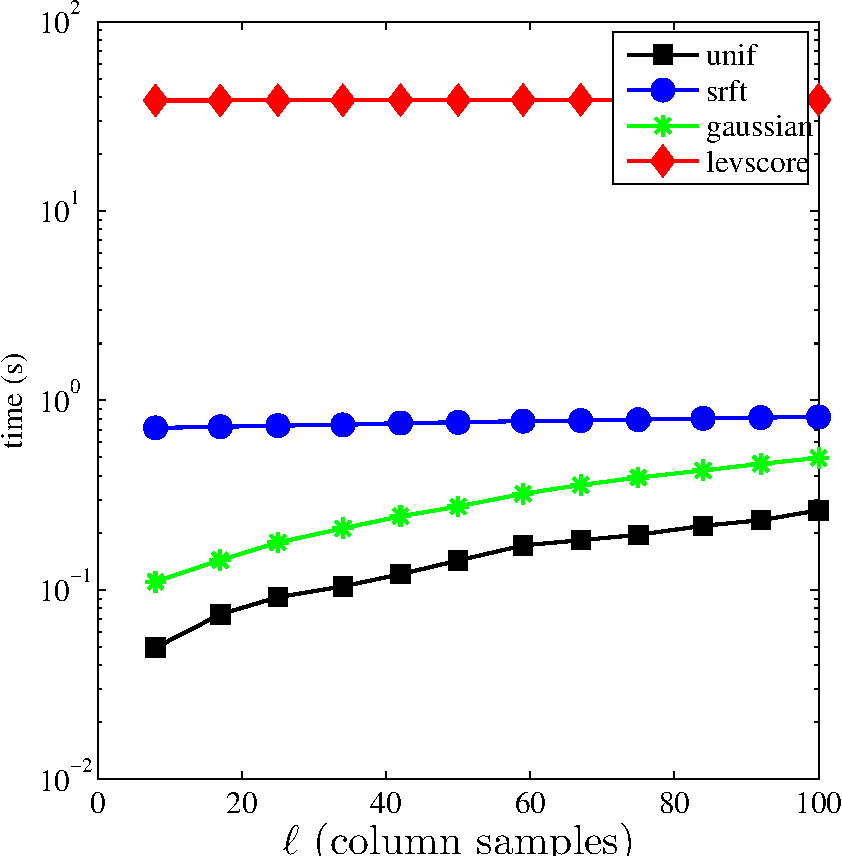
\includegraphics[width=1.5in,keepaspectratio=true]{figures/spsd/Dexterrank8exact-methods-timings.pdf}%
%    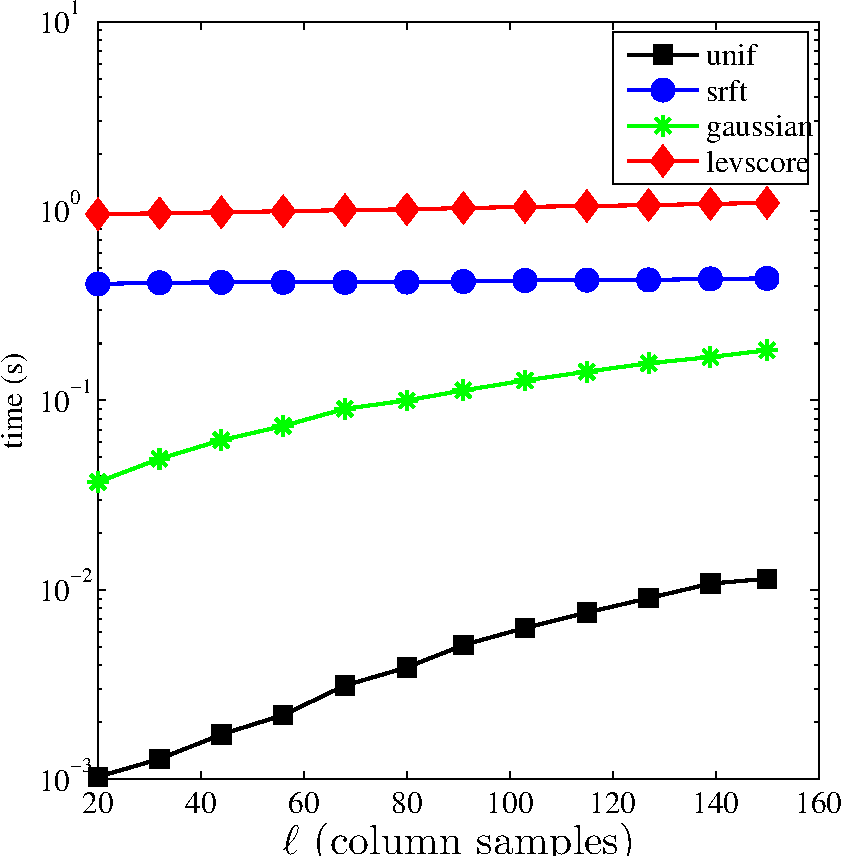
\includegraphics[width=1.5in,keepaspectratio=true]{figures/spsd/Abalonesigma1exact-methods-timings.pdf}%
%    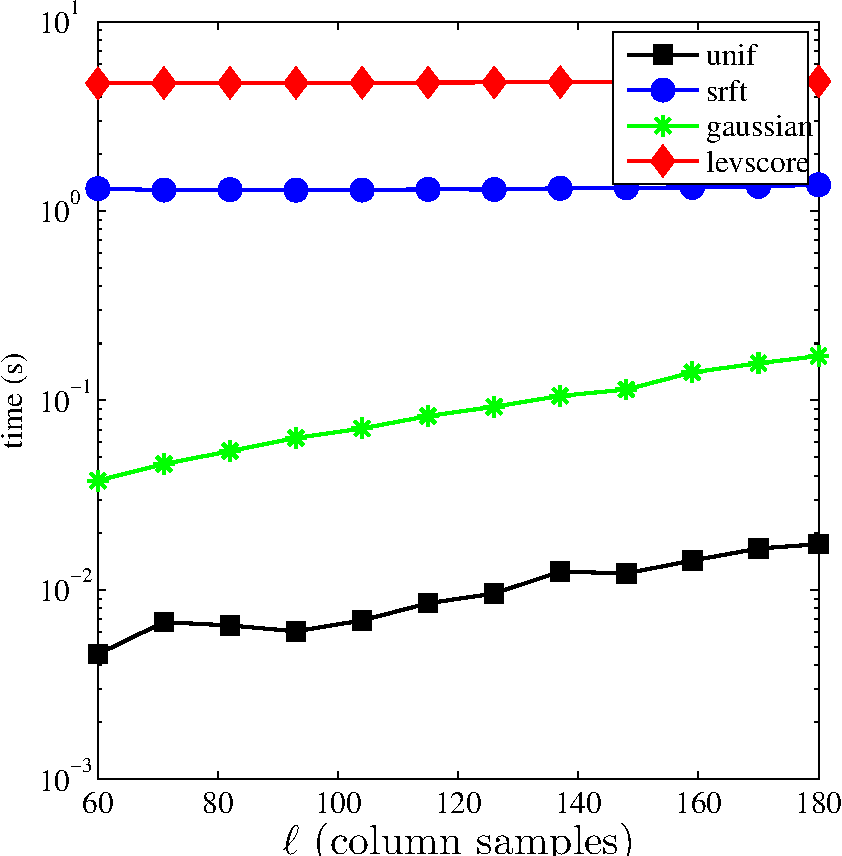
\includegraphics[width=1.5in,keepaspectratio=true]{figures/spsd/Enronrank60exact-methods-timings.pdf}}
% Left to right, computation times for the sketches of the Dexter, Abalone, and Enron matrices.
% \begin{itemize}
%  \item The fact that Dexter is a linear kernel (i.e. $\matA = \matX \matX\transp$ for some $\matX\transp$)
%   allows us to speed up the computation of $\matA \matS.$
%  \item We used the $\const{O}(n \log n)$ implementation of the SRFT available in Matlab, 
%   as opposed to the $\const{O}(n \log \ell)$ theoretically possible.
%  \item Gaussian multiplication is more efficient on sparse datasets than SRFT multiplication.
% \end{itemize}
% 
%\end{frame}
% 
% \begin{frame}{Empirical performance (inexact schemes)}
%  Obtaining the exact leverage scores (via QR or SVD) is expensive. We substitute the
%  following approximations:
%  \begin{itemize}
%   \item {\color{dgreen} Power method approximations}. Use the power method to obtain approximate bases for the 
%   dominant $k$-dimensional eigenspace of $\matA.$ Terminate when the leverage scores converge.
%   \item {\color{dgreen} Frobenius-norm approximations}. Use a random projection to quickly construct 
%   a matrix close to $\matA$ in the Frobenius norm, and use the leverage scores of this matrix
%   \refer{Drineas et al. 2012}.
%   \item {\color{dgreen} Spectral-norm approximations}. Use a random projection to quickly
%   construct a matrix close to $\matA$ in the spectral norm, and use the leverage scores of this matrix
%   \refer{Drineas et al. 2012}.
%  \end{itemize}
%  
% 
% \end{frame}
% 
% \begin{frame}
% 
%   \centerline{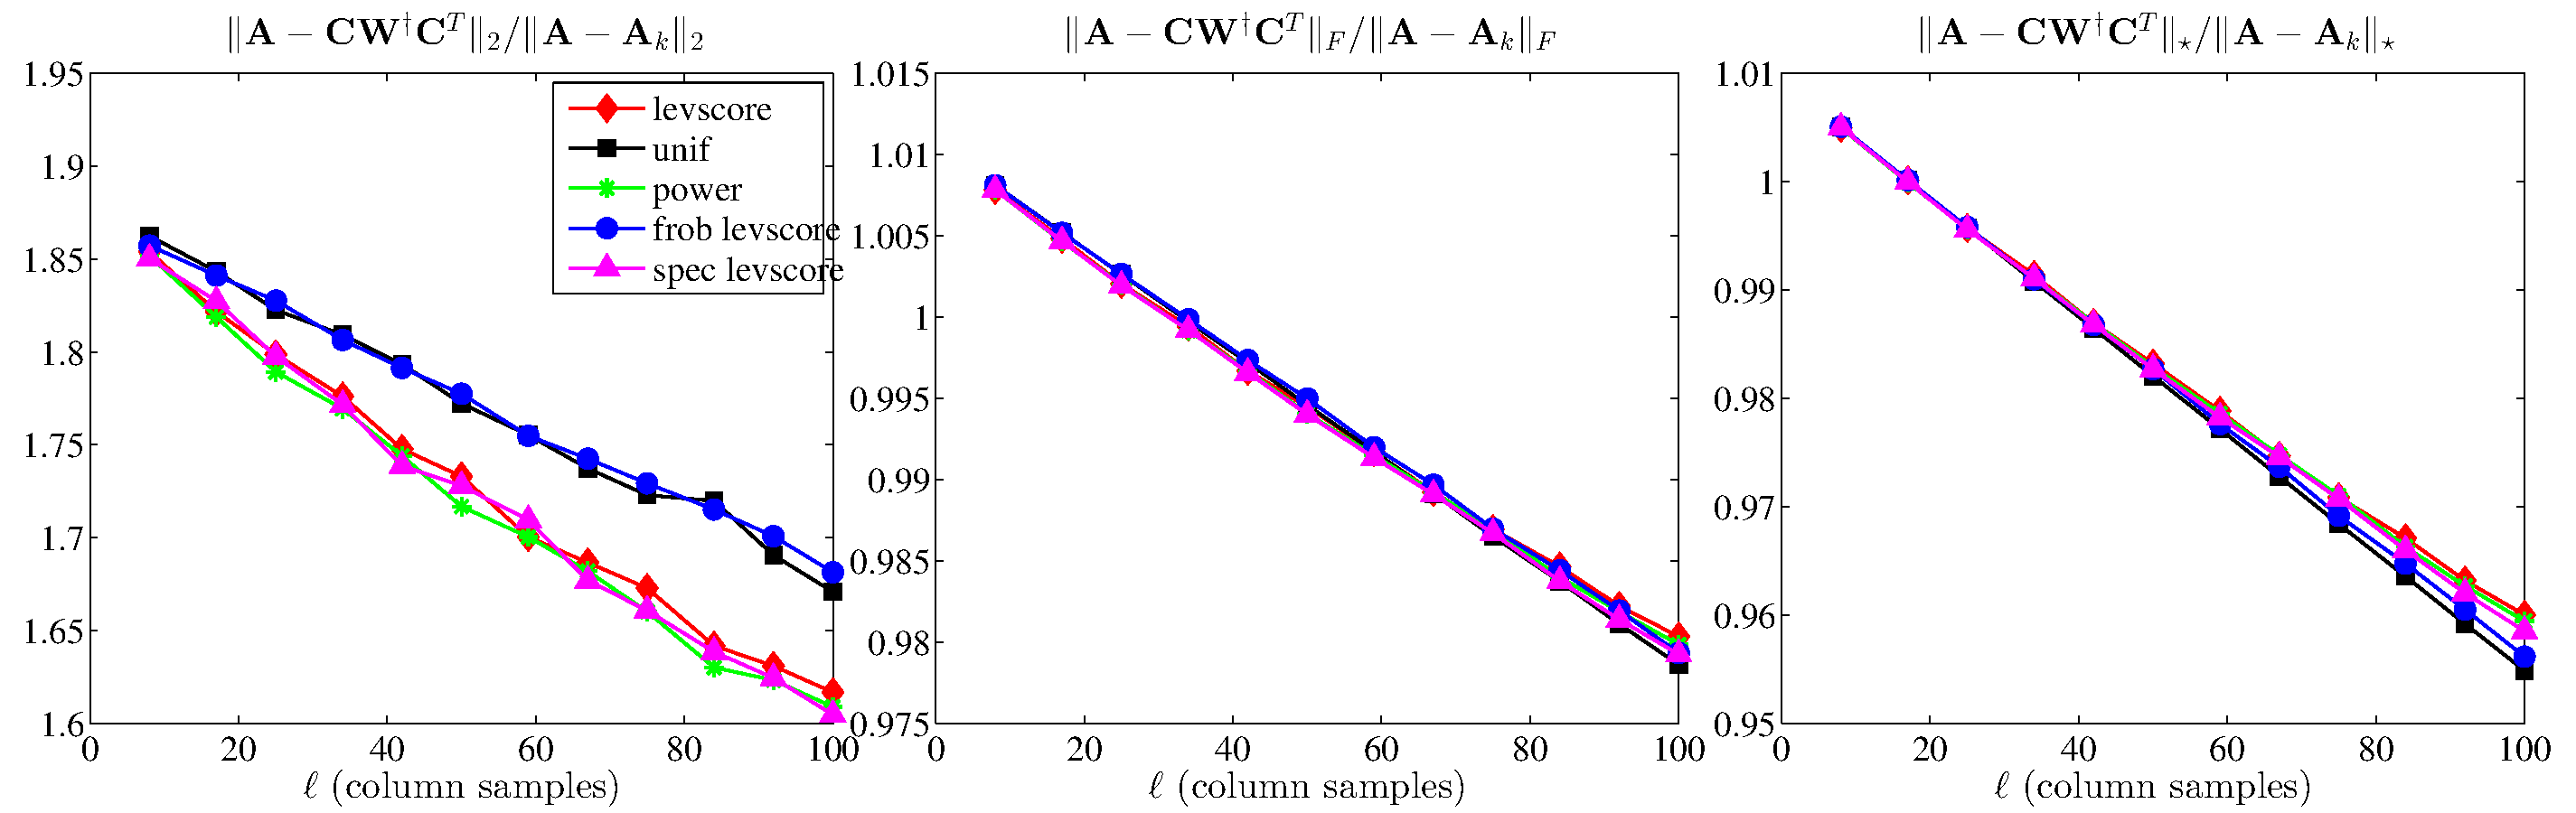
\includegraphics[width=4.7in, keepaspectratio=true]{figures/spsd/Dexterrank8inexact-methods-nonfixed-rank-errors}}
% 
%  Dexter, a $2000 \times 2000$ Gram matrix from the UCI Machine Learning Repository. 
%  Target rank $k= 8.$
% \end{frame}
% 
% \begin{frame}
% 
%   \centerline{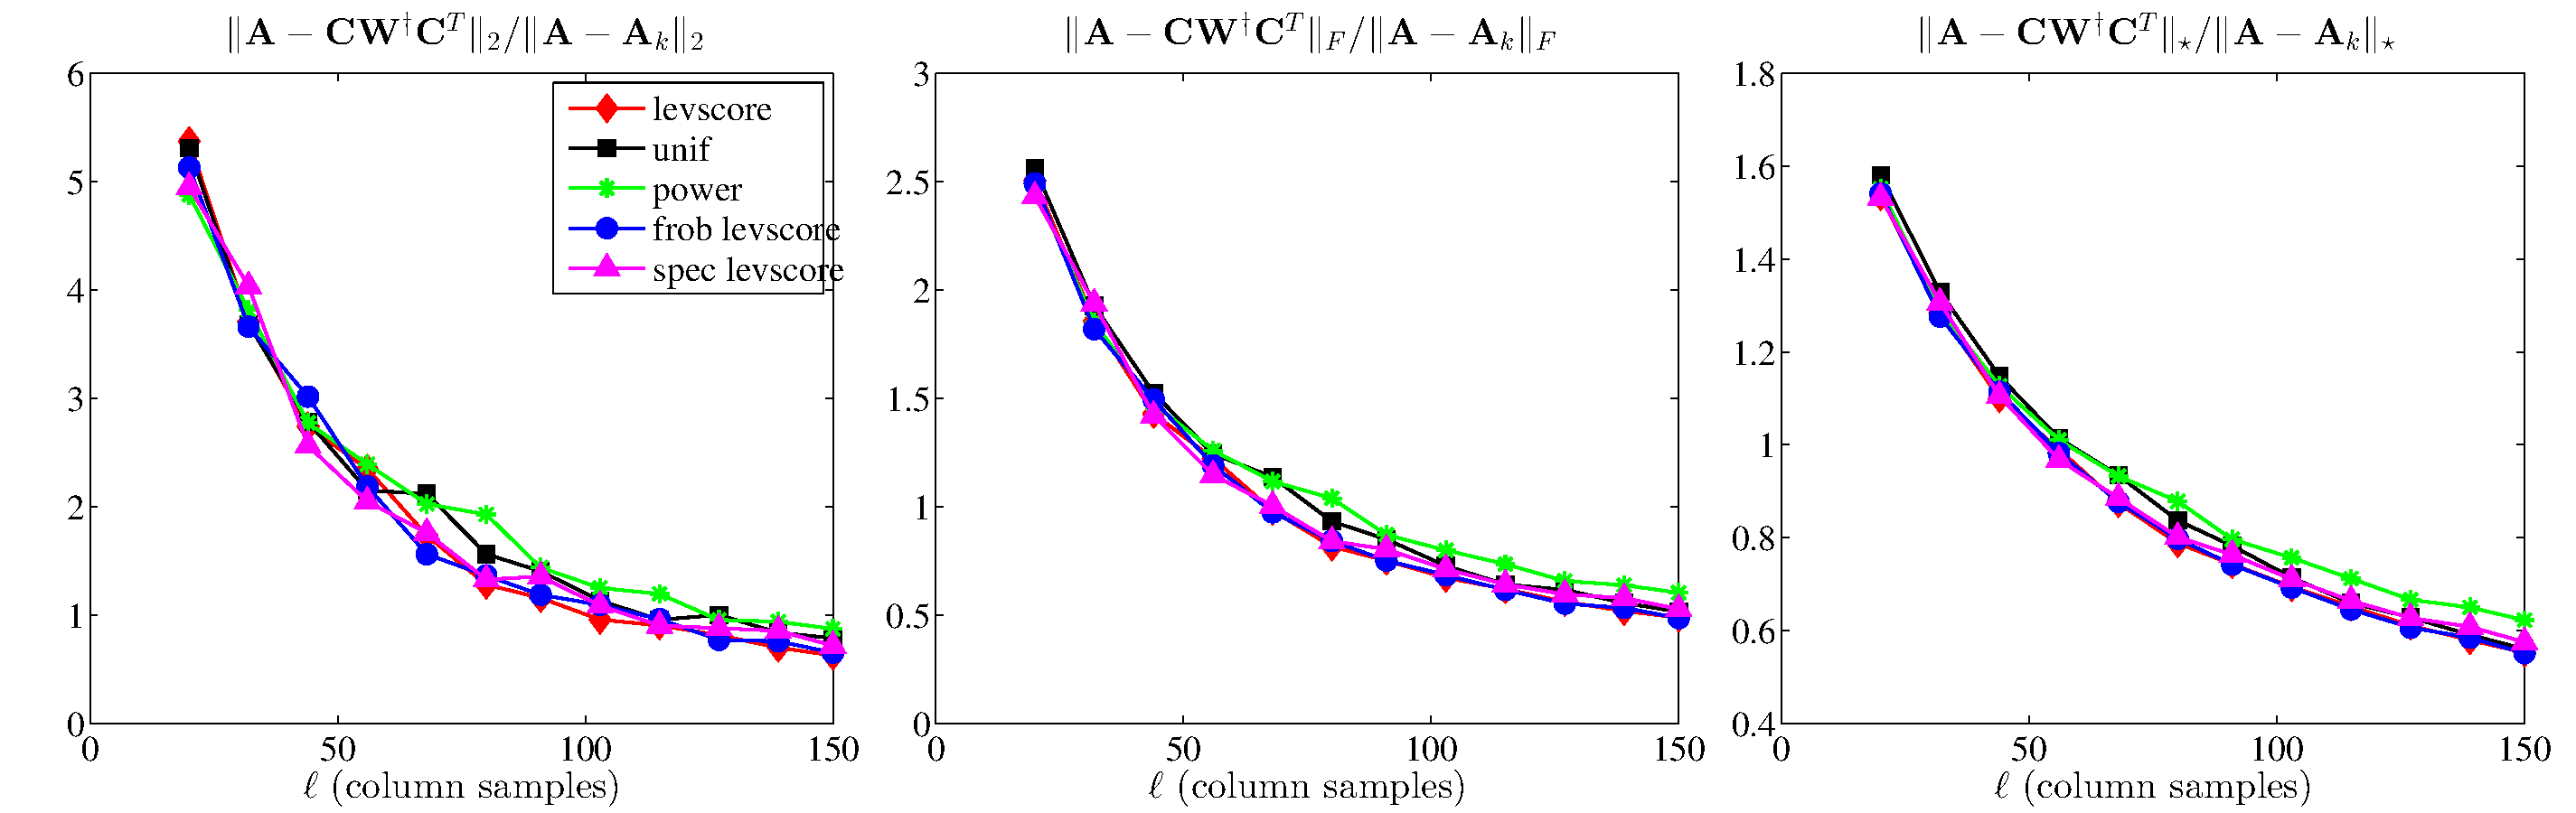
\includegraphics[width=4.7in, keepaspectratio=true]{figures/spsd/Abalonesigma1inexact-methods-nonfixed-rank-errors}}
% 
%  Abalone, a $4898 \times 4898$ Radial Basis Kernel matrix from the UCI Machine Learning Repository. 
%  Target rank $k= 20.$ 
% \end{frame}
% 
% \begin{frame}
%  
%   \centerline{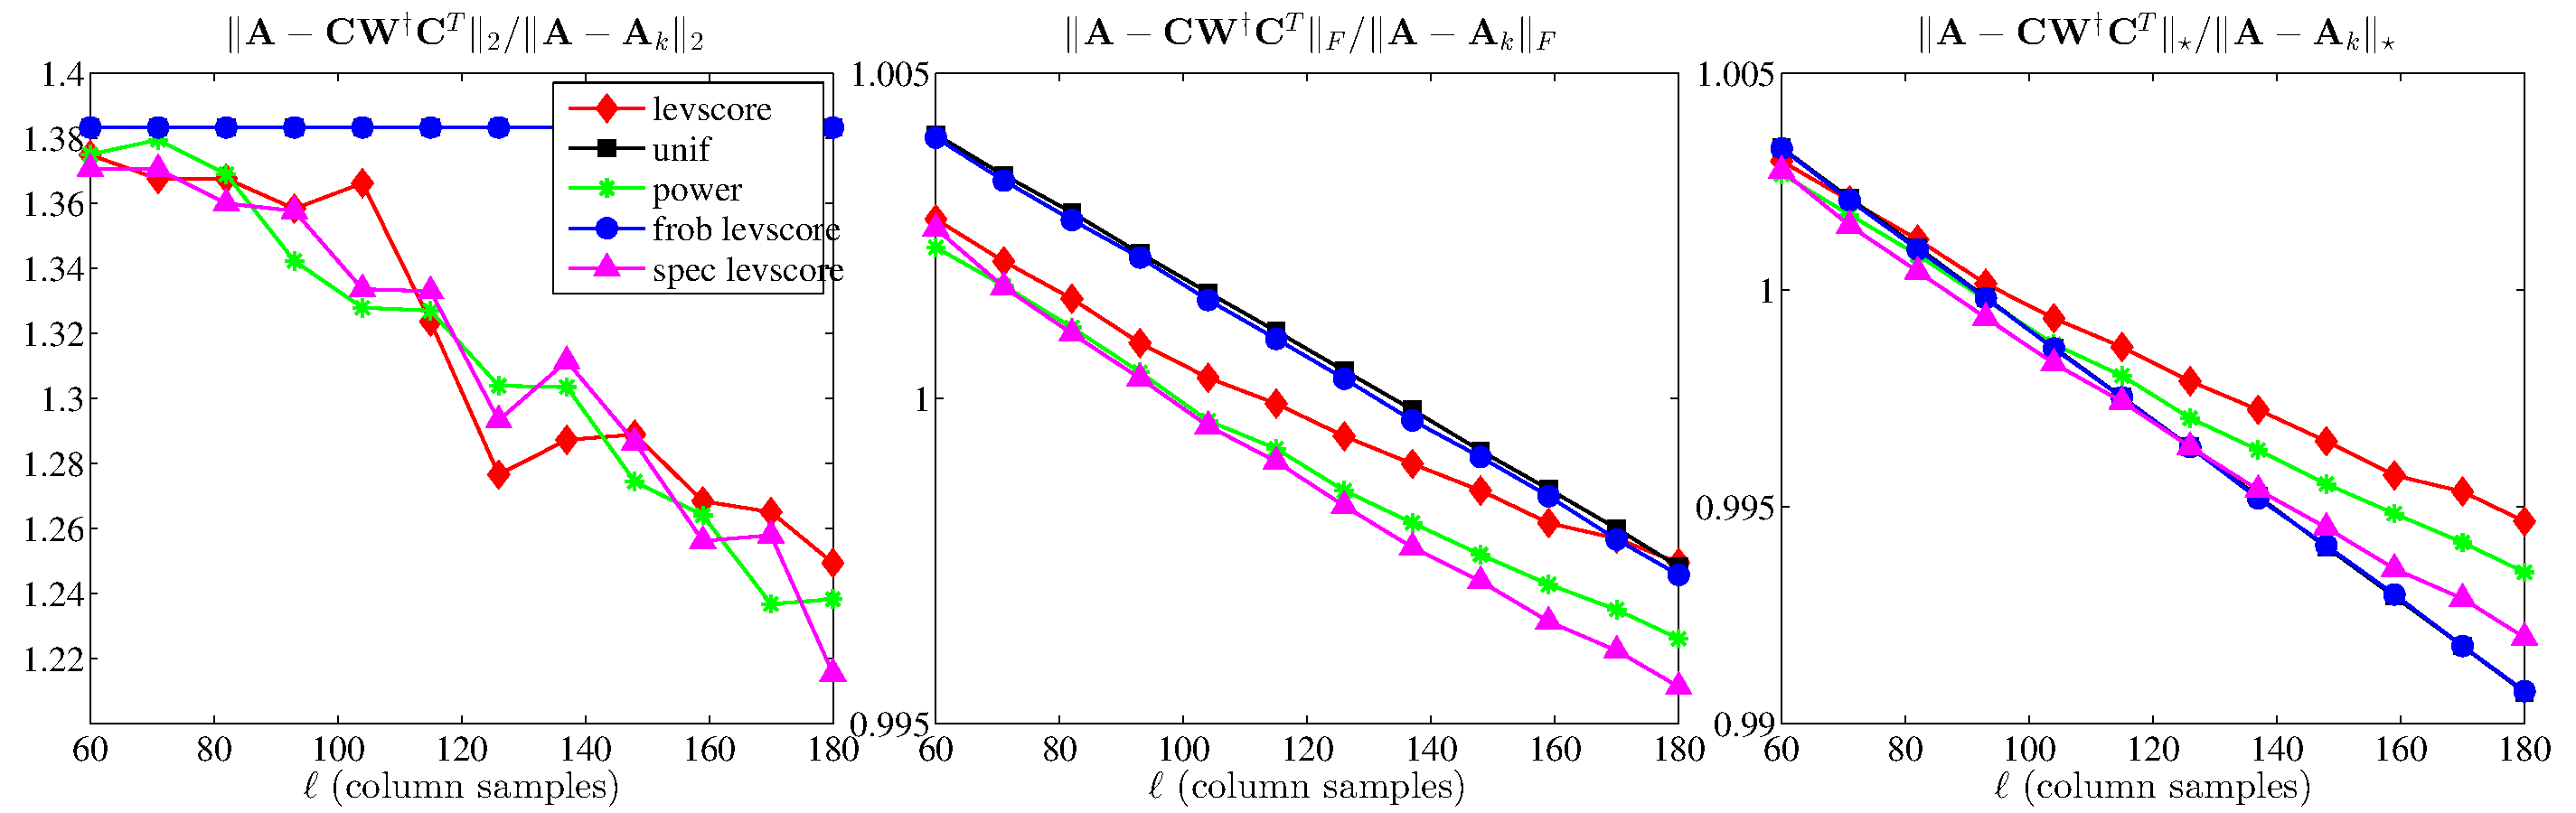
\includegraphics[width=4.5in, keepaspectratio=true]{figures/spsd/Enronrank60inexact-methods-nonfixed-rank-errors}}
%  Enron, a $10K \times 10K$ Graph Laplacian matrix from the Stanford SNAP collection. Target
%  rank $k = 60.$ 
% \end{frame}
% 
% \begin{frame}
%   \centerline{%
%     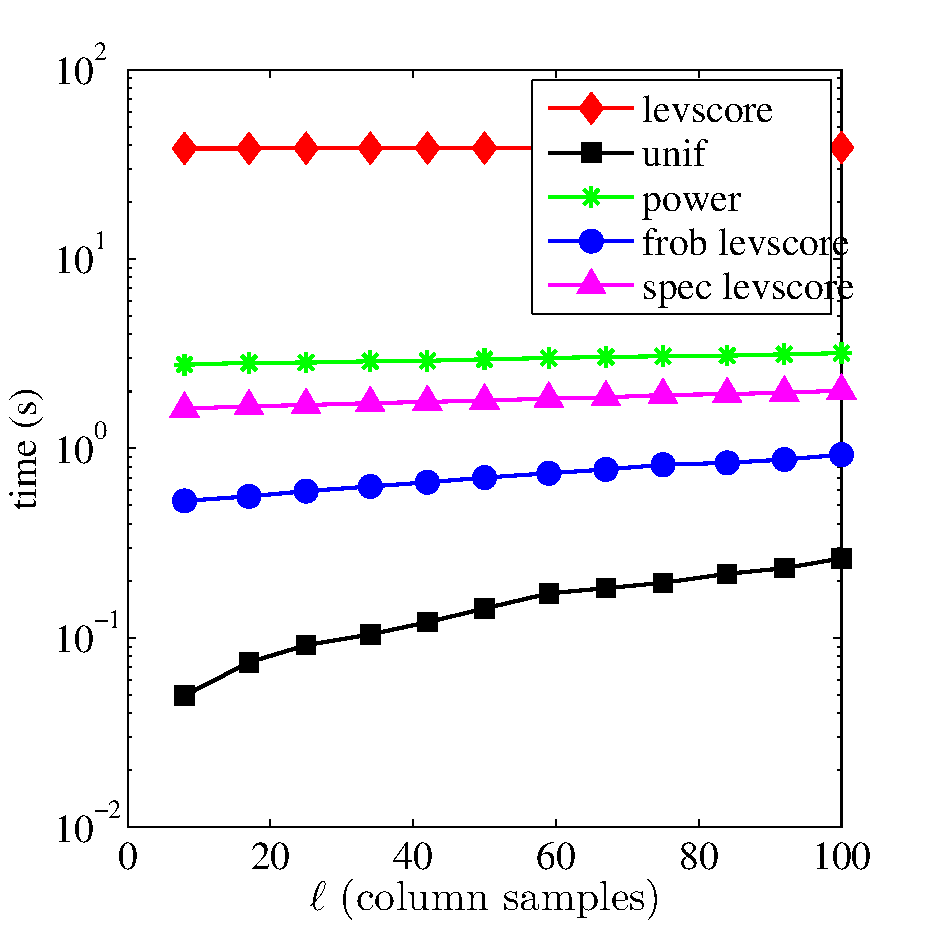
\includegraphics[width=1.5in,keepaspectratio=true]{figures/spsd/Dexterrank8inexact-methods-timings.pdf}%
%     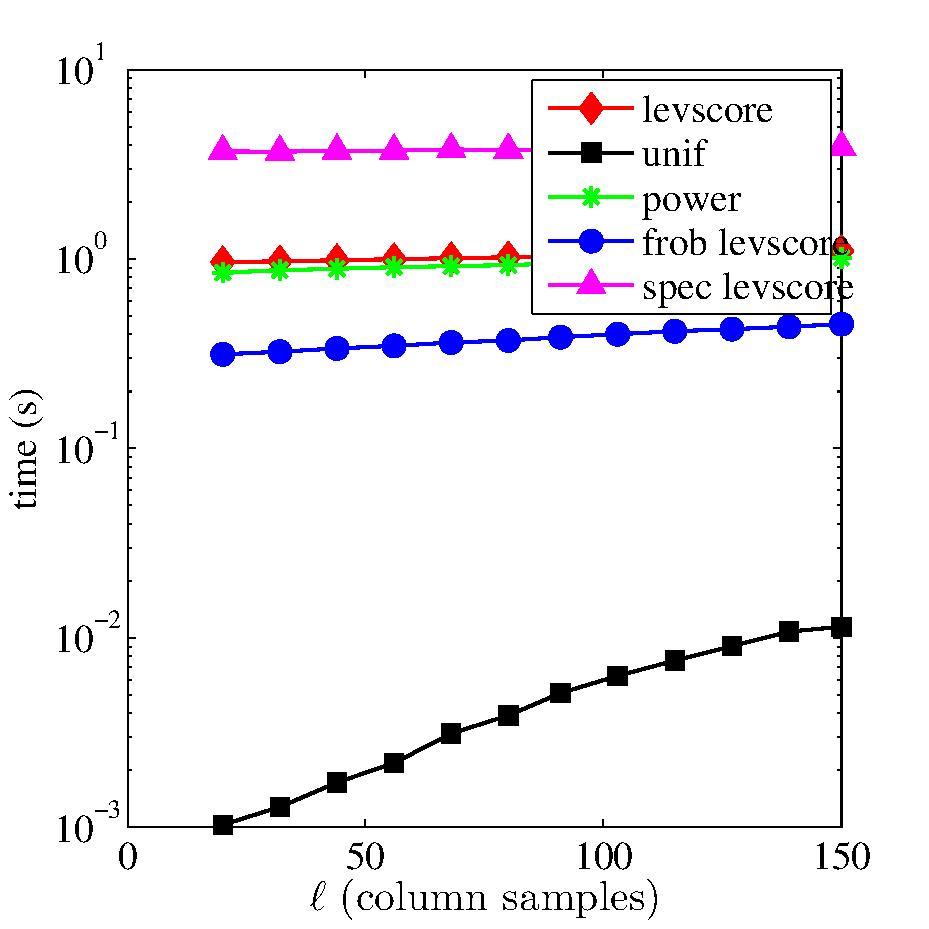
\includegraphics[width=1.5in,keepaspectratio=true]{figures/spsd/Abalonesigma1inexact-methods-timings.pdf}%
%     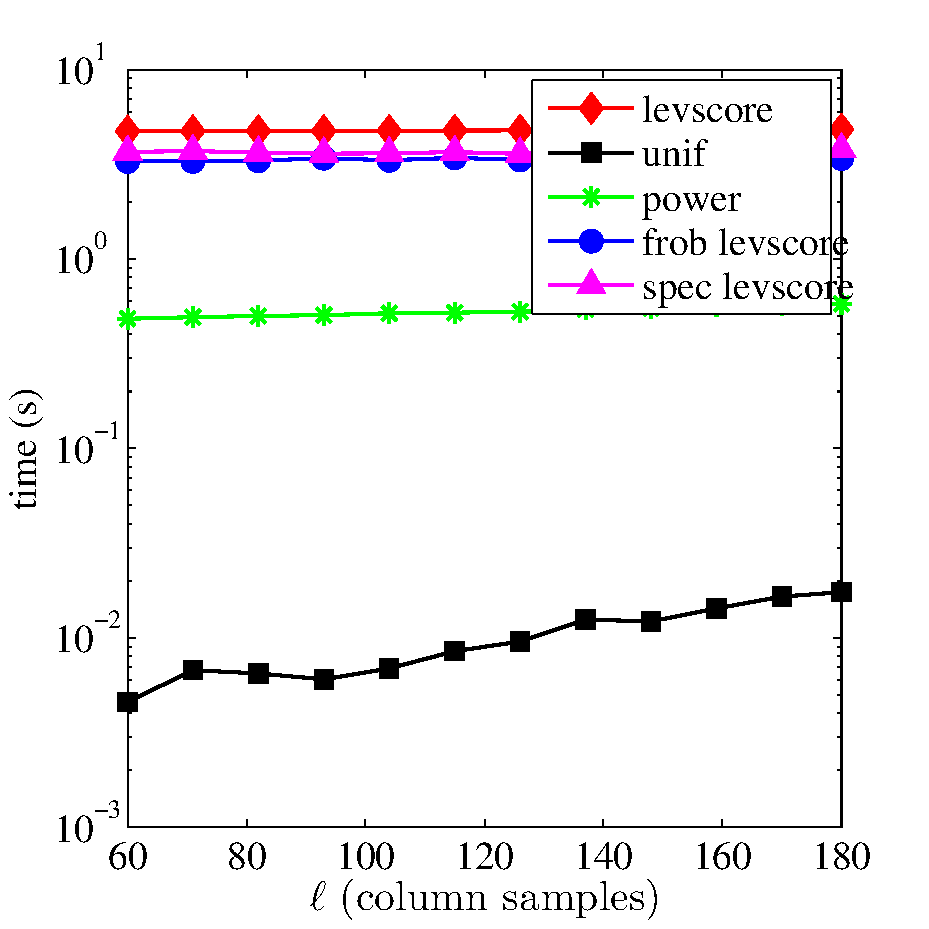
\includegraphics[width=1.5in,keepaspectratio=true]{figures/spsd/Enronrank60inexact-methods-timings.pdf}}
% Left to right, computation times for the sketches of the Dexter, Abalone, and Enron matrices.
% 
% \vspace{0.7em}
% Which approximate leverage score algorithm is appropriate (more efficient than exact leverage
% score computation) depends on the properties of the matrix.
% \end{frame}
% 
%  
% \begin{frame}
% Observations:
% \begin{itemize}
%  \item The leverage sketches are often the most accurate on average, especially when $\ell$ is small. However, variance
%  depends on leverage score distribution and can be high.
%  \item The relative trace-norm errors are all smaller than the relative Frobenius-norm errors, which are in turn 
%  smaller than the relative spectral-norm errors.
%  \item The sketches are more distinguished by their behavior in the spectral norm than the Frobenius or trace norms.
% \end{itemize}
% 
% \end{frame}
% 

\begin{frame}{Prior work}

\centerline{\scriptsize
\begin{tabular}{|l|l|c|}
\hline
Source, sketch & $\ell$ & $\|\matA - \matC\matW^\pinv\matC\transp\|_2$\\
\hline 
\refer{Drineas and Mahoney 2005},          column-sampling & $\Omega(\epsilon^{-4} k)$ & $\|\matA - \matA_k\|_2 + \epsilon \sum_{i=1}^n A_{ii}^2$ \\
\refer{Talwalkar and Rostamizadeh 2010},   Nystr\"om        & $\Omega(\mu k \log k)$    & 0, if $\rank(\matA) = k$ \\
\refer{Kumar et al. 2012},                  Nystr\"om        & $\Omega(1)$               & $\|\matA - \matA_k\|_2 + (n/\sqrt{\ell}) \max_{ii} A_{ii}$ \\
\refer{Chiu and Demanet 2012},             Nystr\"om       & $\Omega(\mu k \log n)$    & $(1 + n/\ell) \|\matA - \matA_k\|_2$ \\
\refer{Chiu and Demanet 2012},             SRFT sketch                & $\Omega(k \log^2 n)$      & $(1 + n/\ell) \|\matA - \matA_k\|_2$ \\
\hline
\end{tabular}
}
\vspace{1em}

\begin{itemize}
 \item The estimated additional error in \refer{Drineas and Mahoney 2005} can be on the order of $\epsilon \tr(\matA).$
 \item The \refer{Talwalkar and Rostamizadeh 2010} exact recovery result requires $\matA$ to be exactly low-rank.
 \item The \refer{Chiu and Demanet 2012} results require $\Omega(k \log n)$ samples as opposed to $\Omega(k \log k).$
       The factor $n/\ell$ is optimal in the Nystr\"om bound, but unnecessary in the SRFT bound.
\end{itemize}

\refer{G. and Mahoney 2013} provides a framework for deriving significantly improved asymptotic error bounds.
\end{frame}

\begin{frame}{Deterministic error bounds for SPSD sketches}
 Recall the partitioned eigendecomposition of $\mat{A}:$
  \[ \mat{A} = \matU \matSig \matU\transp = [\mat{U}_1 \ \ \mat{U}_2] 
  \left[\begin{matrix} \matSig_1 & \\ & \matSig_2 \end{matrix} \right] 
  [\mat{U}_1 \ \ \mat{U}_2]\transp
  \]
  and let
 \[
  \matOmega_1 = \matU_1\transp \matS \quad \text{ and } \matOmega_2 = \matU_2\transp \matS
 \]
 capture the interactions of the sketching matrix with the dominant and residual eigenspaces of $\matA.$
 \vspace{1em}

 Geometrical interpretation (when $\matS$ has orthogonal columns):
 \begin{itemize}
  \item $\matU_1\transp \matS \text{ has full row-rank } \Leftrightarrow \tan(\matU_1, \matS) \neq \infty.$ 
  \item $\bigbar\matOmega_2 \matOmega_1^\pinv\bigbar_2 = \tan(\matU_1, \matS).$
 \end{itemize}
\end{frame}

\begin{frame}
 Our error bounds for SPSD sketches follow from the key observation that 
 \begin{block}{SPSD sketches approximate $\matA^{1/2}$, \refer{G. 2011}}
  \[
   \matC\matW^\pinv \matC\transp = (\matA^{1/2} \matP_{\matA^{1/2} \matS}) (\matP_{\matA^{1/2} \matS} \matA^{1/2}).
  \]
 \end{block}
 
 Corollaries:
 \begin{itemize}
 % \item $\matA - \matC \matW^\pinv \matC\transp \succeq \mat{0}.$
  \item $\matC\matW^\pinv \matC\transp \approx \matA_k$ when the range of $\matA^{1/2} \matS$ is close to the 
 range of the dominant $k$-dimensional eigenspace of $\matA^{1/2},$ spanned by $\matU_1.$
 \item The errors of SPSD sketches are given by: 
 \[
   \|\mat{A} - \mat{C}\mat{W}^\pinv \mat{C}\transp\|_\xi =
   \|\mat{A} - \matA^{1/2} \mat{P}_{\mat{A}^{1/2} \mat{S}} \mat{A}^{1/2}\|_\xi
 \]
 for $\xi \in \{2, \mathrm{F}, \mathrm{tr}\}.$
 \end{itemize}
\end{frame}

\begin{frame} 
 By extending the perturbation arguments of \refer{Halko et al. 2011}, 
 
 \begin{block}{Simplified error bounds from \refer{G. and Mahoney 2013}}
 If $\matOmega_1 = \matU_1\transp \matS$ has full row rank, then
 \begin{align*}
 \|\matA - \matC \matW^\pinv \matC\transp\|_2 & \leq \left(1 + \bigbar\matOmega_2 \matOmega_1^\pinv\bigbar_2^2\right) \|\matA - \matA_k\|_2 , \\
 \|\matA - \matC \matW^\pinv \matC\transp\|_\rf & \leq \|\matA - \matA_k\|_\rf + 2\sqrt{2} 
 \bigbar {\matOmega_2 \matOmega_1^\pinv} \bigbar_2^2 \cdot \tr(\matA - \matA_k), \text{ and } \\
 \tr(\matA - \matC \matW^\pinv \matC\transp) & \leq 
  \left(1+ \bigbar { \matOmega_2 \matOmega_1^\pinv} \bigbar_2^2 \right) \cdot \tr(\matA - \matA_k)
 \end{align*}
 \end{block}
 
 The randomness of $\matS$ enters only through the sketching interaction matrix  ${\matOmega_2 \matOmega_1^\pinv},$
 so these bounds can be used for arbitrary sampling schemes. Recall that
 \[
   \bigbar\matOmega_2 \matOmega_1^\pinv\bigbar_2 = \tan(\matU_1, \matS).
 \]

\end{frame}

 
 \begin{frame}{Application: Gaussian sketches}

  \begin{block}{Gaussian sketches \refer{G. and Mahoney 2013}}
  If $\ell = \Omega((1 + \epsilon^{-1}) k),$ then
  \begin{align*}
   \|\matA - \matC \matW^\pinv \matC\transp\|_2 & \leq (1 + \epsilon) \|\matA - \matA_k\|_2 + \frac{\epsilon}{k}\tr(\matA - \matA_k), \\
  \|\matA - \matC \matW^\pinv \matC\transp\|_\rf & \leq \|\matA - \matA_k\|_\rf + \sqrt{\epsilon \|\matA - \matA_k\|_2 \tr(\matA - \matA_k)} \\
  & \quad \quad \quad  + \sqrt{\frac{\epsilon}{k}}\tr(\matA - \matA_k), \text{ and} \\
   \tr(\matA - \matC \matW^\pinv \matC\transp) & \leq (1 + \epsilon)\tr(\matA - \matA_k).
  \end{align*}
  with probability at least $1 - k^{-1} - \e^{-k\epsilon^{-1}}.$
  \end{block}

  This and similarly improved bounds for the other SPSD sketches follow from our deterministic bounds and analyses of the
  sketching interaction matrices available for the different choices of $\matS.$
\end{frame}
%  \begin{frame}{Spectral error bounds}
%   \begin{block}{Leverage sketches}
%   If $\ell = \Omega(\epsilon^{-1} k \log(k/\delta))$, then 
%   \[
%    \|\matA - \matC \matW \matC\transp\|_2 \leq \|\matA - \matA_k\|_2 + \epsilon \tr(\matA - \matA_k)
%   \]
%   with probability at least $1 - \delta - 0.4.$
%  \end{block}
%  
%  \begin{block}{SRFT sketches}
%    If $k = \Omega(\log n)$ and $\ell = \Omega(\epsilon^{-2}k \log(n/\delta))$, then
%    \[
%   \|\matA - \matC \matW \matC\transp\|_2 \leq \left( 5 + \frac{\epsilon}{\sqrt{k}}\right) \|\matA - \matA_k\|_2 
%    + \frac{\epsilon^2}{k} \tr(\matA - \matA_k)
%   \]
%   with probability at least $1 - \delta.$
%  \end{block}
% 
% \end{frame}
% 
% \begin{frame}
% 
%  \begin{block}{Gaussian sketches}
%   If $\ell = \Omega((1 + \epsilon^{-1}) k),$ then
%   \[
%    \|\matA - \matC \matW \matC\transp\|_2 \leq (1 + \epsilon) \|\matA - \matA_k\|_2 + \frac{\epsilon}{k}\tr(\matA - \matA_k)
%   \]
%   with probability at least $1 - k^{-1} - \e^{-k\epsilon^{-1}}.$
%   \end{block}
%   
% \end{frame}

%  \begin{frame}{Error bounds for leverage sketches}
%   \begin{block}{\refer{G. and Mahoney 2013}}
%   If $\ell \geq 6400 \epsilon^{-1} k \log(k/\delta)$ where $\epsilon \in (0,1)$ and $\delta \in (0,1),$ then 
%   \begin{align*}
%    \|\matA - \matC \matW \matC\transp\|_2 & \leq \|\matA - \matA_k\|_2 + (\epsilon \tr((\matA - \matA_k)^{2p-1}))^{1/(2p-1)} \\
%    \|\matA - \matC \matW \matC\transp\|_\rf & \leq \|\matA - \matA_k\|_\rf + \sqrt{\epsilon} \gamma^{p-1} \tr(\matA - \matA_k) \\
%    \tr(\matA - \matC \matW^\pinv \matC\transp) & \leq (1 + \epsilon \gamma^{2p-2}) \tr(\matA - \matA_k)
%   \end{align*}
%   simultaneously, with probability at least $1 - 6 \delta - 0.6.$
%  \end{block}
%  
%  \begin{itemize}
%   \item Follows from the deterministic bounds and the analysis of $\bigbar \matSig_2^{1/2} \matOmega_2 \matOmega_1^\pinv\bigbar_\rf$ when $\matS$
%    corresponds to leverage sketching given in (Mackey et al. 2012).
%   \item The large constant 6400 and the failure probability (bounded away from zero) are artifacts of the analysis.
%  \end{itemize}
%  \end{frame}
 
%  \begin{frame}{Error bounds for SRFT sketches}
%   \begin{block}{(G. and Mahoney, 2013)}
%    If $\ell \geq 24 \epsilon^{-1} [\sqrt{k} + \sqrt{8\log(8n/\delta)}]^2 \log(8k/\delta),$ where $\epsilon \in (0,1/3)$ and
%    $\delta \in (0,1),$ then
%    \begin{align*}
%   \|\matA - \matC \matW \matC\transp\|_2 & \leq \|\matA - \matA_k\|_2 \\
%   & + 
%   \const{O}\left(\frac{\log(n/\delta)}{(1- \sqrt{\epsilon}) \ell} \right)^{1/(2p-1)} \tr((\matA - \matA_k)^{2p-1})^{1/(2p-1)} \\
%    \|\matA - \matC \matW \matC\transp\|_\rf & \leq \|\matA - \matA_k\|_\rf + 16 \sqrt{\epsilon} \gamma^{p-1} \tr(\matA - \matA_k) \\
%    \tr(\matA - \matC \matW^\pinv \matC\transp) & \leq (1 + 11 \epsilon \gamma^{2p-2}) \tr(\matA - \matA_k)
%   \end{align*}
%   simultaneously, with probability at least $1 - 2\delta.$
%   \end{block}
% 
%   \begin{itemize}
%   \item Follows from our deterministic bounds and analyses of $\bigbar \matSig_2^{1/2} \matOmega_2 \matOmega_1^\pinv\bigbar_{2,\rf}$ when $\matS$
%    is an SRFT, adapted from (Boutsidis and G., 2012).
%   \end{itemize}
%  \end{frame}

%  \begin{frame}{Error bounds for Gaussian sketches}
%  \begin{block}{(G. and Mahoney, 2013)}
%   If $\ell \geq (1 + 963 \epsilon^{-1}) k,$ where $\epsilon \in (0,1],$ then
%   \begin{align*}
%    \|\matA - \matC \matW \matC\transp\|_2 & \leq (1 + \epsilon) \|\matA - \matA_k\|_2 + \frac{\epsilon}{k}\tr((\matA - \matA_k)^{(2p-1)})^{1/(2p-1)} \\
%    \|\matA - \matC \matW \matC\transp\|_\rf & \leq \|\matA - \matA_k\|_\rf + 19 \gamma^{p-1} \sqrt{\epsilon \|\matA - \matA_k\|_2 \tr(\matA - \matA_k)}\\
%                   & \quad +  3 \gamma^{p-1} \sqrt{\frac{\epsilon}{k}} \tr(\matA - \matA_k)\\
%    \tr(\matA - \matC \matW^\pinv \matC\transp) & \leq (1 + \gamma^{2p-2} \epsilon) \tr(\matA - \matA_k) 
%   \end{align*}
%   simultaneously, with probability at least $1 - 2k^{-1} - 4\e^{-963k\epsilon^{-1}}.$
%   \end{block}
%   \begin{itemize}
%    \item Follows from our deterministic bounds and analyses of $\bigbar \matSig_2^{1/2} \matOmega_2 \matOmega_1^\pinv\bigbar_{2,\rf}$ when $\matS$
%    consists of i.i.d. $\mathcal{N}(0,1)$ random variables given in (Halko et al. 2011).
%   \end{itemize}
% 
%  \end{frame}
 
 
%  \begin{frame}
%   \begin{block}{Frobenius- and trace-norm error bounds \refer{G. and Mahoney 2013}}
%    If $\ell \geq 8 \mu k \log(k/\delta),$ then
%    \[
%     \|\matA - \matC \matW^\pinv \matC\transp\|_\rf \leq  \|\matA - \matA_k\|_\rf + \frac{4}{\delta^2}  \tr(\matA - \matA_k)
%    \]
%    and
%    \[
%     \tr(\matA - \matC \matW^\pinv \matC\transp) \leq \left(1 + \frac{2}{\delta^2}\right) \tr(\matA - \matA_k)
%    \]
%    hold simultaneously with probability at least $1 - 4\delta.$
%   \end{block}
% 
%  \end{frame}

% \begin{frame}{Random projections vs SPSD sketches}
%   \refer{Halko et al. 2011} mentions approximating SPSD matrices with $\matP_{\matA \matS} \matA \matP_{\matA \matS},$ which requires two passes over $\matA.$ 
% \begin{itemize} 
%  \item $\matP_{\matA\matS} \matA \matP_{\matA \matS}$ is $(\mat{P}_{{\color{red} \matA}\matS} \matA^{1/2})(\matA^{1/2} \matP_{{\color{red} \matA} \matS}).$
%  \item The ``two-pass sketch'' $(\matA^2 \matS) (\matS\transp \matA^3 \matS)^\pinv (\matS\transp\matA^2)$ is 
%  $(\matA^{1/2} \matP_{{\color{red} \matA^{3/2}} \matS})(\matP_{{\color{red} \matA^{3/2}}\matS} \matA^{1/2} ).$
% \end{itemize}
% 
% \centerline{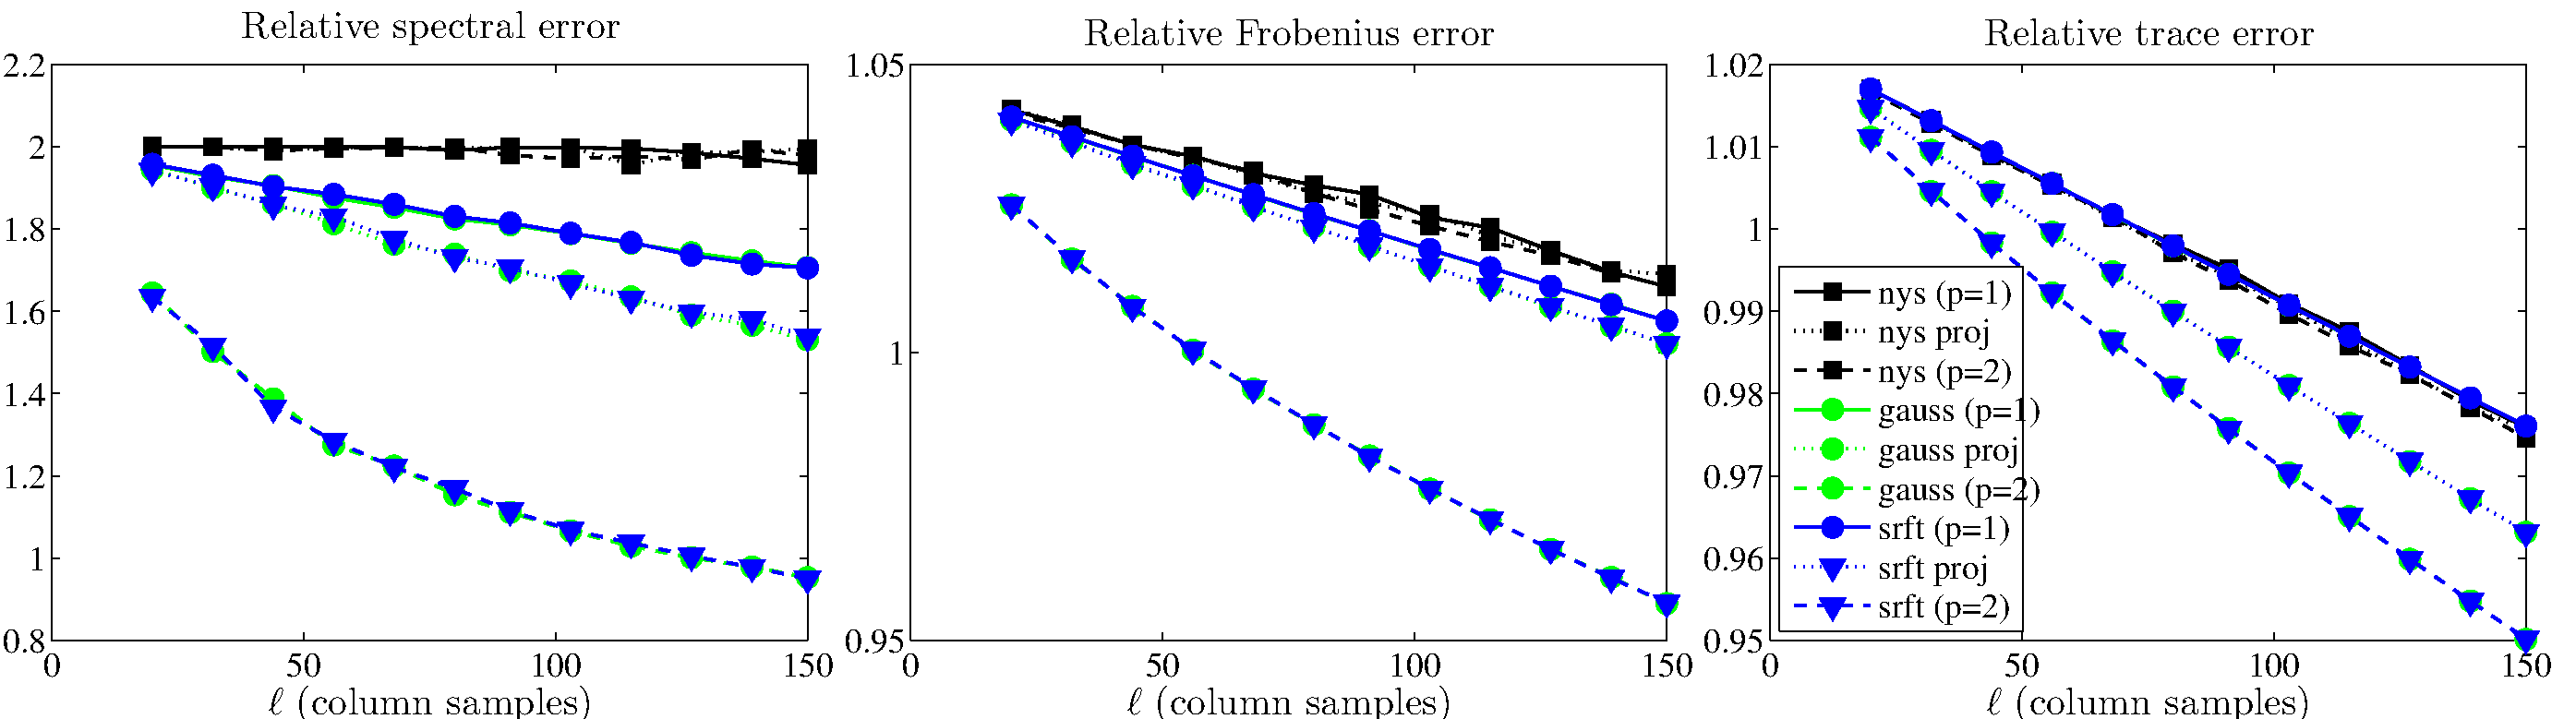
\includegraphics[width=4.7in, keepaspectratio=true]{figures/spsd/Winecompactsigma1-eigexact-methods-nonfixed-rank-errors-with-eig}}
% 
% Wine, a $4898\times4898$ sparse Radial Basis Kernel matrix from the UCI Machine Learning Respository. Target rank $k=20.$ Each
% point is the average relative error over 30 trials.
% \end{frame}
% 
% \begin{frame}{Conclusion}
%  Identified and analyzed a class of low-rank SPSD approximations generalizing the Nystr\"om extension.
%   \begin{itemize}
%        \item Provided deterministic error bounds and theoretical error guarantees for several types of randomized
%     SPSD sketches.
%     \item Established an optimal relative-error spectral-norm bound for Nystr\"om extensions.
%     \item Provided empirical evidence that SPSD sketches perform well on a wide range of matrices
%     that arise in machine learning.
%     \item Demonstrated empirically that two-pass SPSD sketches have lower approximation error than the projection-based approximations
%     considered in \refer{Halko et al. 2011}.
%    \end{itemize}
%
% \end{frame}
%
%\begin{frame}
%   Paper ID: 785.
%   \vspace{0.7em}
%   
%   Additional References: (preprints on arXiv)
%  \begin{itemize}
%   \item ``The spectral norm error of the na\"ive Nystr\"om extension'', \refer{Gittens 2011}.
%   \item ``Improved matrix algorithms via the Subsampled Randomized Hadamard Transform'', \refer{Boutsidis and G. 2012}. SIMAX to appear.
%   \item ``Revisiting the Nystr\"om Method for Improved Large-Scale Machine Learning'', \refer{G. and Mahoney 2013}. Submitted.
%   \item Nystr\"om Bestiary (Matlab code for experiments with SPSD sketches)
%          \url{http://users.cms.caltech.edu/~gittens/nystrombestiary/}
%  \end{itemize}
%
% \end{frame}

\section{Polynomial RFMs}

\begin{frame}
\vfill
\begin{beamercolorbox}[center]{}
  \Large \textsc{Polynomial random feature maps for fast kernel learning}
\end{beamercolorbox}
\vfill
\end{frame}

\begin{frame}
\begin{itemize}
\item \textbf{Goal}: Learn non-linear classifiers using linear methods and non-linear feature mappings
\item \textbf{Challenge}: How to deal with an extremely large number of non-linear features?
\item \textbf{Solution}: The kernel trick\\
\begin{center}
$\Phi: \mathbb{R}^d \rightarrow \mathcal{H}$
\end{center}
defines a kernel function $\textrm{K}(\mathbf{x},\mathbf{y})$ by
\begin{center}
    $\textrm{K}(\mathbf{x},\mathbf{y}) = \langle \Phi(\mathbf{x}),\Phi(\mathbf{y}) \rangle_\mathcal{H}, \quad \forall\, \mathbf{x}, \mathbf{y} \in \mathbb{R}^d$
\end{center}

\item Using $\textrm{K},$ a classifier $\mathbf{H}$ is then learned for some $\mathbf{w} \in \mathcal{H}$, where 
\begin{center}
$\mathbf{H}: \mathbf{x} \mapsto \langle \mathbf{w}, \Phi(\mathbf{x})\rangle = \sum_{i=1}^n \alpha_i \mathbf{K}(\mathbf{x}_i, \mathbf{x})$
\end{center}
\end{itemize}
\end{frame}


%%%%%%%%%%%%%%%%
\begin{frame}
\frametitle{The Troubles With Kernels}
\begin{itemize}
    \item \textbf{Dual formulation:} Allows using kernel instead of feature maps, but requires dealing with an $n \times n$ matrix; expensive and possibly can't hold in memory
    \item \textbf{Curse of support}: the number of data points used in $\mathbf{w}$ can grow unboundedly with the training data size $\Rightarrow$ applying classifier $\mathbf{H}$ is expensive
\item \textbf{Solution}: Randomized Features Maps (RFM)\\
\begin{center}
$\textbf{Z}: \mathbb{R}^d \rightarrow \mathbb{R}^{\textrm{\textrm{D}}}$
\end{center}
such that $\forall$ $\mathbf{x}, \mathbf{y} \in \mathbb{R}^d$
\begin{center}
$\langle \textbf{Z}(\mathbf{x}), \textbf{Z}(\mathbf{y}) \rangle \approx \textrm{K}(\mathbf{x},\mathbf{y})$
\end{center}
Use $\mathbf{Z}$ as a feature map in primal formulations
\item RFMs can be used to approximate several classes of kernels
\end{itemize}
\end{frame}

\begin{frame}{Polynomial KRR}
  We focus on RFMs for the polynomial kernel:
\begin{center}
$\textrm{K}(\mathbf{x},\mathbf{y})$ := $(\langle \mathbf{x}, \mathbf{y} \rangle$$+q)^r = \langle [\sqrt{q}, \mathbf{x}], [\sqrt{q}, \mathbf{y}] \rangle^r$
\end{center}
where $q \in \mathbb{R}^{+}$ and $r \in \mathbb{N}_{0}$

\begin{itemize}
    \item The explicit feature map 
        \begin{center}
            $x \mapsto (1, x_1^r, x_2^r, \ldots, x_1^2 x_2 \cdots x_{r-1}, \ldots)$
        \end{center}
        is \emph{extremely} high-dimensional
      \item RFM approaches (\refer{Kar--Karnick 2012} and TensorSketch \refer{Pagh--Pham 2013}) waste capacity: $\mathrm{D}$ is larger than desirable, theoretically and empirically.
    
    \item \textcolor{red}{Our contributions:}
        \begin{enumerate}
            \item \textcolor{red}{A scheme to generate more efficient random features}
            \item\textcolor{red}{A much refined analysis of the Kar--Karnick RFM}
        \end{enumerate}
\end{itemize}

\end{frame}

%%%%%%%%%%%%%%%%

\begin{frame}{Kar--Karnick RFMs}
  Let $\mathbf{w}$ be a vector of random signs. Then
  \[
    \mathbb{E}\langle \mathbf{w}, \mathbf{x} \rangle \langle \mathbf{w}, \mathbf{y} \rangle = \mathbf{x}^{\mathrm{T}} \mathbb{E} (\mathbf{w} \mathbf{w}^{\mathrm{T}}) \mathbf{y} = \langle \mathbf{x}, \mathbf{y}^1 \rangle. 
  \]
  Likewise,
  \[
    \mathbb{E}\left[ \left(\prod_{i=1}^r \langle \mathbf{w}_i, \mathbf{x} \rangle \right) \left(\prod_{j=1}^r \langle \mathbf{w}_j, \mathbf{y} \rangle \right) \right] = \langle \mathbf{x}, \mathbf{y} \rangle^r.
  \]
  So $z : \mathbf{x} \mapsto \left(\prod_{i=1}^r \langle \mathbf{w}_i, [\sqrt{q}, \mathbf{x}] \rangle \right)$ is a RFM for the polynomial kernel: 
  \[
    \mathbb{E} \big( z(\mathbf{x}) \cdot z(\mathbf{y}) \big) = (\langle \mathbf{x}, \mathbf{y} \rangle + q )^r.
  \]

  A better performing RFM can be obtained using i.i.d. copies of this random map $z$:
  \[
    \textbf{Z} : \mathbf{x} \mapsto \frac{1}{\sqrt{D}} ( z_1(\mathbf{x}), \ldots, z_{D}(\mathbf{x})).
  \]
\end{frame}

\begin{frame}
  Another view: let $\mathbf{W}_i \in \mathbb{R}^{\mathrm{D} \times (d+1)}$ be a matrix of random signs for $i=1,\ldots, r$.
\begin{center}
  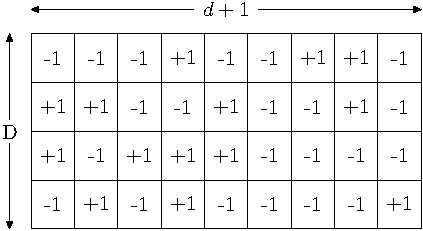
\includegraphics[height=1.2in]{figures/craftmaps/alex_illust/kk}
\end{center}
Then
    $\textbf{Z} : \mathbf{x} \mapsto \frac{1}{\sqrt{D}} (\mathbf{W}_1 [\sqrt{q}, \mathbf{x}]) \odot (\mathbf{W}_2 [\sqrt{q}, \mathbf{x}]) \odot \cdots \odot (\mathbf{W}_r [\sqrt{q}, \mathbf{x}]).$
\end{frame}

\begin{frame}{TensorSketch polynomial RFMs}
    \textbf{Def}: A CountSketch matrix $\mathbf{C} : \mathbb{R}^d \rightarrow \mathbb{R}^{\textrm{D}}$ has one nonzero entry per column
    that is $\pm 1$ with equal probability \\
\begin{center}
  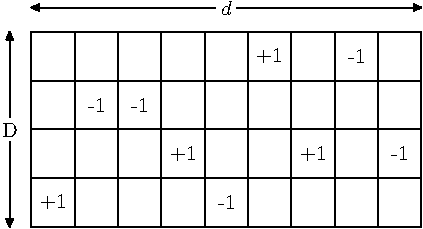
\includegraphics[height=1.2in]{figures/craftmaps/alex_illust/countsketch}
\end{center}
\vspace{-.25cm}

\refer{Pagh--Pham 2013} show that if $\mathbf{C}_i$ for $i=1, \ldots, r,$ are independent CountSketch matrices, then 
\[
  \textbf{Z} : \mathbf{x} \mapsto \frac{1}{\sqrt{D}} \mathbf{F}^{-1} \cdot
    \left( (\mathbf{F} \mathbf{C}_1 [\sqrt{q}, \mathbf{x}]) \odot \cdots \odot 
    (\mathbf{F} \mathbf{C}_r [\sqrt{q}, \mathbf{x}]) \right)
\]
is a polynomial RFM.
\end{frame}

\begin{frame}
\frametitle{How many KK random features?}
\begin{itemize}
  \item Fix two arbitrary points on the unit sphere in $\mathbb{R}^d;$ consider $\mathrm{K}(\mathbf{x}, \mathbf{y}) = \langle \mathbf{x}, \mathbf{y} \rangle^r.$
\item How many random features are needed to approximate the kernel function at those points: $|\mathrm{K}(\mathbf{x},\mathbf{y}) - \langle \mathbf{Z}(\mathbf{x}), \mathbf{Z}(\mathbf{y})\rangle| < \varepsilon$?
\item \textcolor{blue}{Original estimate from Kar--Karnick 2012: $\mathrm{D} \gtrsim \varepsilon^{-2} d^{2r}.$}
\item There are substantially fewer degree-$r$ monomials in $d$ features: $\binom{d+r-1}{r}.$

\end{itemize}
\end{frame}

\begin{frame}

By carefully estimating the moments of $|\mathrm{K}(\mathbf{x}, \mathbf{y}) - \langle \mathbf{Z}(\mathbf{x}), \mathbf{Z}(\mathbf{y})\rangle|,$
we show that \textcolor{red}{$\mathrm{D}$ is independent of the input dimensionality:  $\mathrm{D} \gtrsim 4^r \varepsilon^{-2}$  suffices.}

\begin{block}{Uniform kernel approximation \refer{G et al. 2014}}
Let $\mathbf{X} \subset \mathbb{R}^d$ be a set of $n$ unit vectors. If $\mathrm{D} \gtrsim (4 \log(n)^2 )^{r+1} \varepsilon^{-2},$ then with constant probability
$$\max_{\mathbf{x}, \mathbf{y} \in \mathbf{X}} |\mathrm{K}(\mathbf{x}, \mathbf{y}) - \langle \mathbf{Z}(\mathbf{x}), \mathbf{Z}(\mathbf{y})\rangle| < \varepsilon$$
\end{block}

Thus the $\mathrm{D}$ needed for a fixed point-wise accuracy grows polylogarithmically in the number of data points.

\end{frame}

%%%%%%%%%%%%%%%%
% \begin{frame}
% \frametitle{Random Feature Maps -- Overview}
% \begin{figure}[b]
% \centering
%     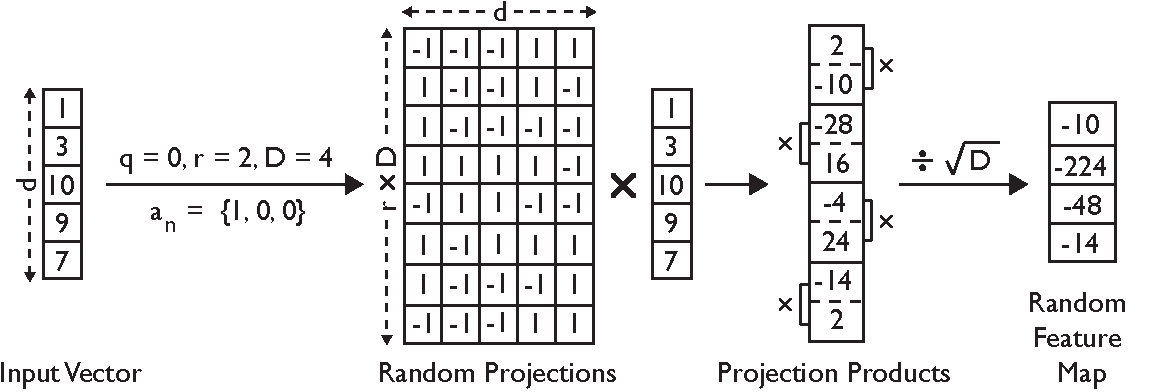
\includegraphics[width=0.9\textwidth]{kar_illust}
%   \caption{\small{Projection of a $5$ dimensional vector to a random feature map for a $2^{\textrm{nd}}$ order homogenous polynomial kernel in $4$ dimensions. As $a_{n}$ = $\{1, 0, 0\}$ here, we need $r \times \textrm{D} = 2 \times 4 =8$ Rademacher vectors such that we could multiply each $r=2$ projections to construct $\mathbf{Z}$ in $\textrm{D}=4$ dimensions.}}
% \label{fig:kar_illust}
% \end{figure}
% \end{frame}
% 
%%%%%%%%%%%%%%%%
\begin{frame}
\frametitle{Polynomial RFMs -- Limitations}
\begin{figure}[b]
\centering
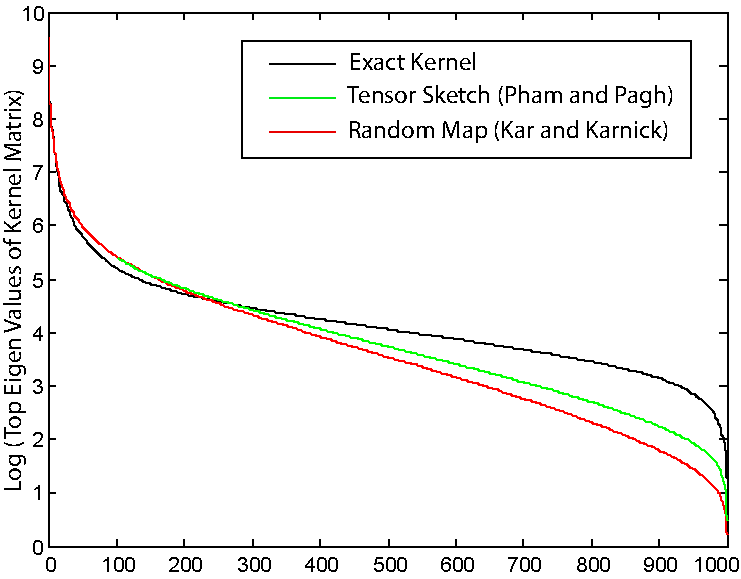
\includegraphics[width=0.65\textwidth]{figures/craftmaps/rank_def}
\\Rank deficiency of TensorSketch and Random Feature Maps
\end{figure}
\end{frame}

%%%%%%%%%%%%%%%%
\begin{frame}
\begin{figure}[b]
\centering
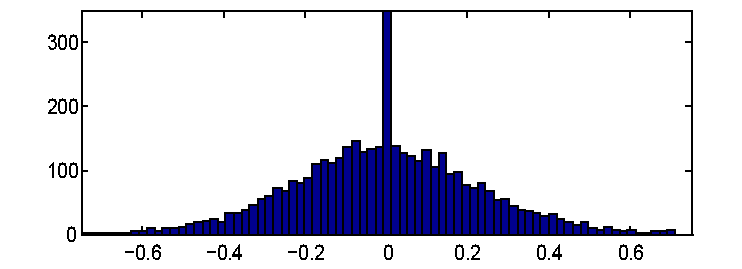
\includegraphics[width=0.75\textwidth]{figures/craftmaps/w1}
  \caption*{\small{Histograms of weight vectors for MNIST two-class classifier learned using a $2^{12}$ dimensional Random Feature Map}}
\label{fig:w1}
\end{figure}
\end{frame}


%%%%%%%%%%%%%%%%
\begin{frame}
\begin{itemize}
\item \textbf{Dilemma}: To approximate $\textrm{K}(\mathbf{x},\mathbf{y})$ accurately, $\textrm{D}$ might have to be increased to undesirably large values.
\item \textbf{Opportunity}: since $\textbf{Z}$ is rank-deficient, the same information can be encoded in fewer than $\mathrm{D}$ random
    linear combinations of its entries.

\begin{center}
    \begin{tikzpicture}
      \node[anchor=south west, inner sep=0] (image) at (0,0) {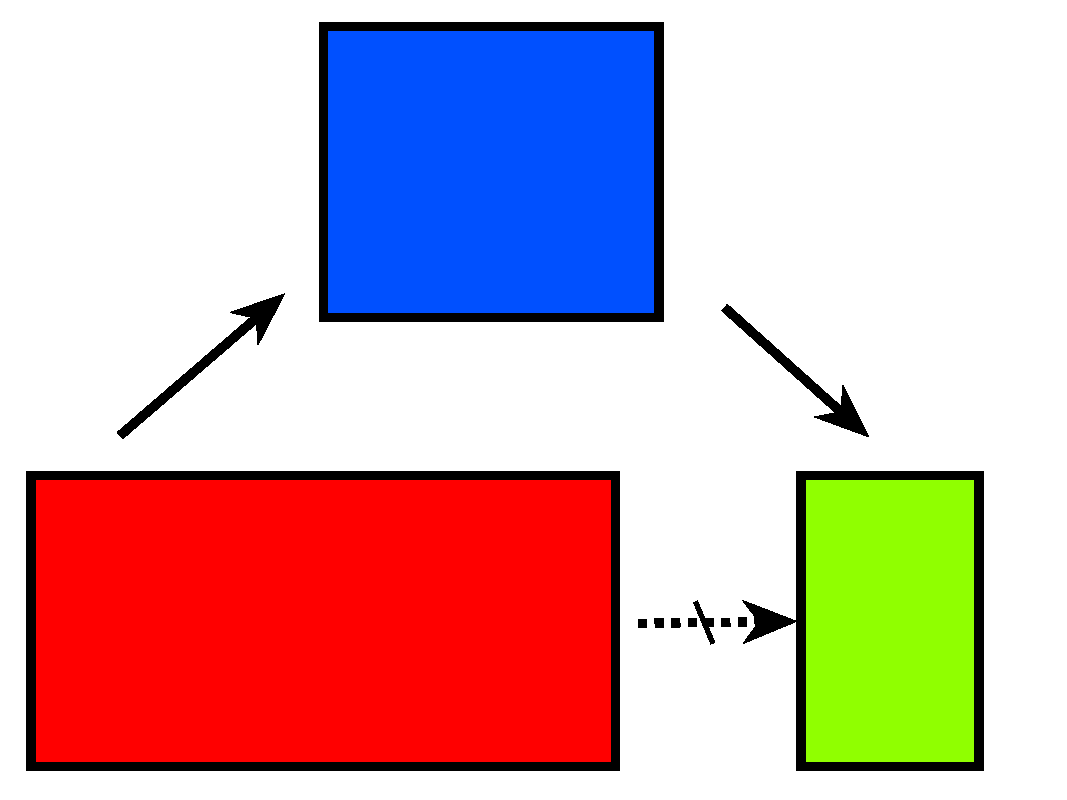
\includegraphics[width=3in]{figures/craftmaps/updown}};
        \node[align=center,font={\Huge}] at (2.3, 1.2) {$\mathbb{R}^d$};
        \node[align=center,font={\Huge}] at (3.5, 4.5) {$Z$};
        \node[align=center] at (6.35, 1.2) {$\mathbf{R}\cdot \mathbf{Z}$};
    \end{tikzpicture}
\end{center}
\end{itemize}
\end{frame}


%%%%%%%%%%%%%%%%

\begin{frame}
\begin{algorithm*}[H]
\caption{{\sc -- CRAFTMaps}}
\label{alg:craftmaps}
{\bf Input:} $q,$ $r,$ and $\textrm{D}$ and $\textrm{E}$ satisfying $\textrm{E} < \textrm{D}$\\
{\bf Output:} CRAFTMap $\textbf{G}: \mathbb{R}^d \rightarrow \mathbb{R}^{\textrm{E}}$, such that $\langle\textbf{G}(\mathbf{x}), \textbf{G}(\mathbf{y})\rangle \approx \textrm{K}(\mathbf{x},\mathbf{y})$\\
\begin{algorithmic}
    \State \textbf{Up Project}: Construct $\textbf{Z}: \mathbb{R}^d \rightarrow \mathbb{R}^{\textrm{D}}$ so that $\langle\textbf{Z}(\mathbf{x}), \textbf{Z}(\mathbf{y})\rangle \approx \textrm{K}(\mathbf{x},\mathbf{y})$
    \State \textbf{Down Project}: Let $\mathbf{R}$ be a JLT from $\mathbb{R}^{\textrm{D}}$ to $\mathbb{R}^{\textrm{E}}$ and set $\textbf{G} = \mathbf{R} \cdot \textbf{Z}.$
%     \vspace{0.15cm}
\end{algorithmic}
\end{algorithm*}

Since $\mathbf{R}$ is a JLT,
\begin{center}
    $\langle \textbf{G}(\mathbf{x}), \textbf{G}(\mathbf{y}) \rangle \approx 
     \langle \textbf{Z}(\mathbf{x}), \textbf{Z}(\mathbf{y}) \rangle \approx 
     \textrm{K}(\mathbf{x},\mathbf{y}).$
\end{center}

\emph{NB}: In our experiments, we take $\mathbf{R}$ to be a Subsampled Randomized Hadamard Transform matrix for speed.
\end{frame}

%%%%%%%%%%%%%%%%
\begin{frame}
    \frametitle{Improvement with CRAFTMaps}
    \begin{center}
      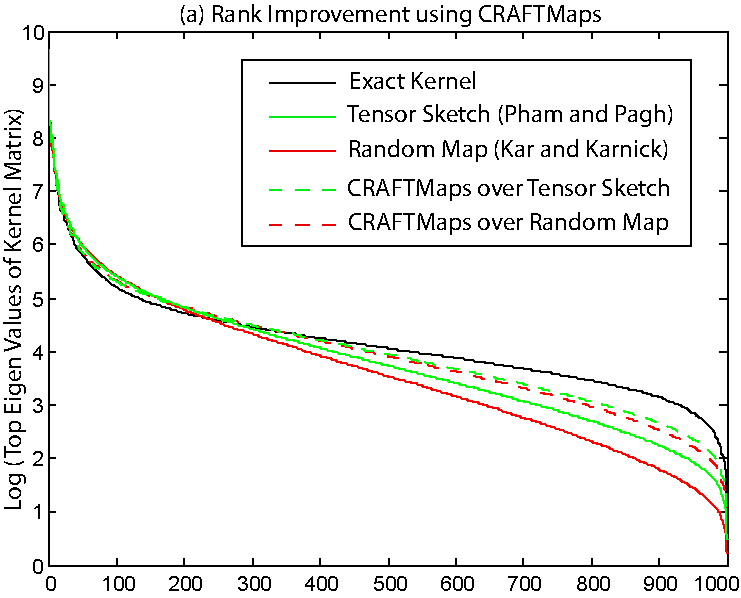
\includegraphics[width=0.75\textwidth]{figures/craftmaps/rfm_limitations_01}
    \end{center}
\end{frame}

\begin{frame}
    \begin{figure}
    \begin{center}
      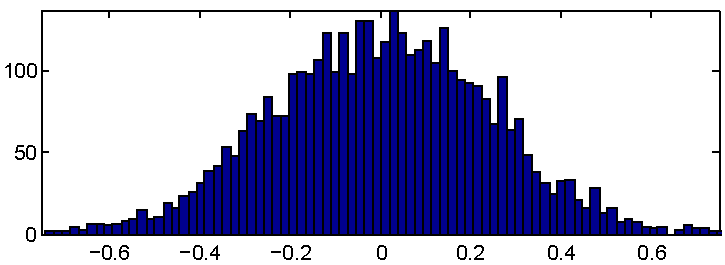
\includegraphics[width=0.75\textwidth]{figures/craftmaps/w2}
    \caption*{Histogram of weight vectors for MNIST data learned using a $2^{12}$ dimensional KK-RFM with $\mathrm{D}=2^{14}.$}
    \end{center}
    \end{figure}
\end{frame}

%%%%%%%%%%%%%%%%
\begin{frame}
\begin{figure}[h]
    \begin{center}
      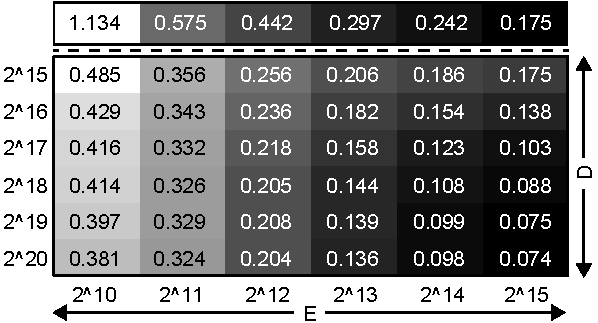
\includegraphics[width=0.8\textwidth]{figures/craftmaps/recon_mnist}
        \caption*{\small NRMSE for polynomial kernel reconstruction using $r=7$ and $q=1$ on MNIST. Top row is for KK-RFM and the bottom table is for CRAFTMaps on KK-RFM.}
    \end{center}
    \end{figure}
\end{frame}

\begin{frame}
    \frametitle{CRAFTMaps vs RFMs: Kernel Approximation}
    \begin{center}
      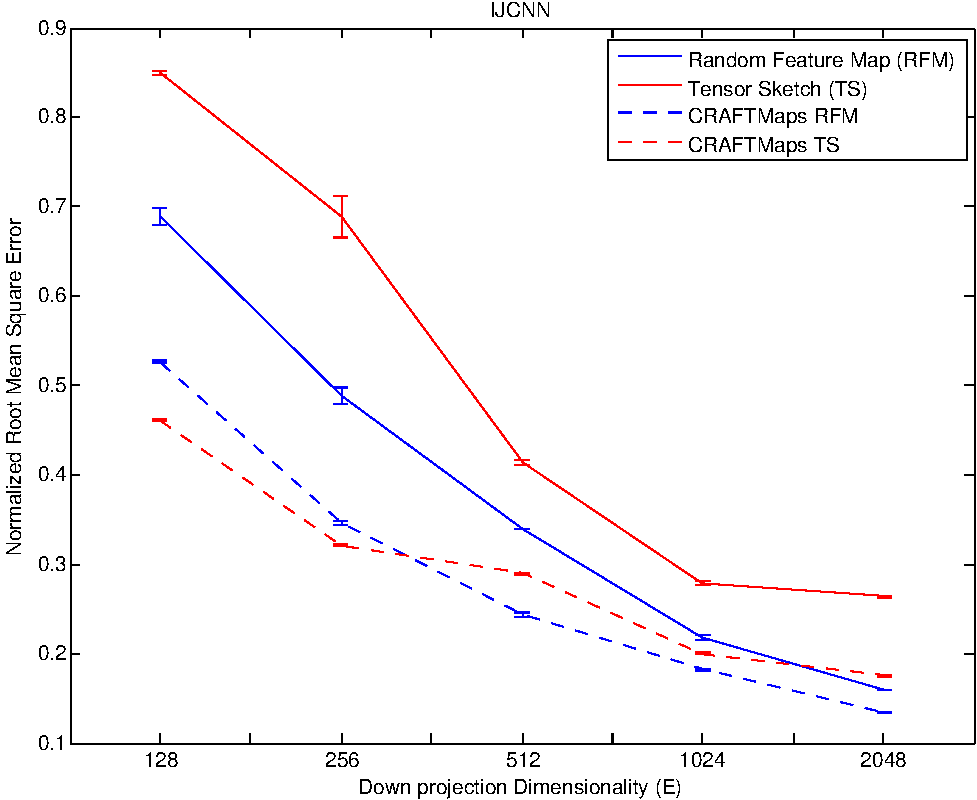
\includegraphics[width=0.75\textwidth]{figures/craftmaps/ijcnn}
    \end{center}
\end{frame}

\begin{frame}
    \begin{center}
      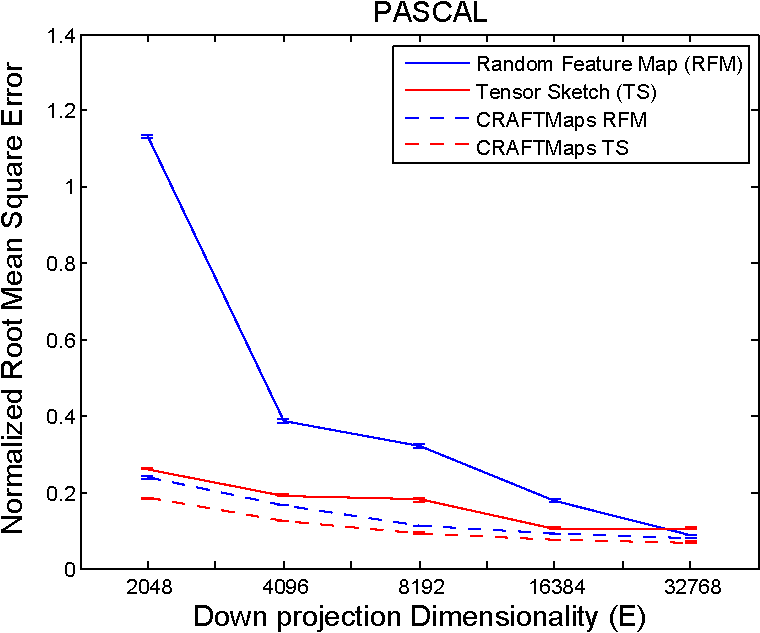
\includegraphics[width=0.75\textwidth]{figures/craftmaps/pascal}
    \end{center}
\end{frame}

\begin{frame}
    \begin{center}
      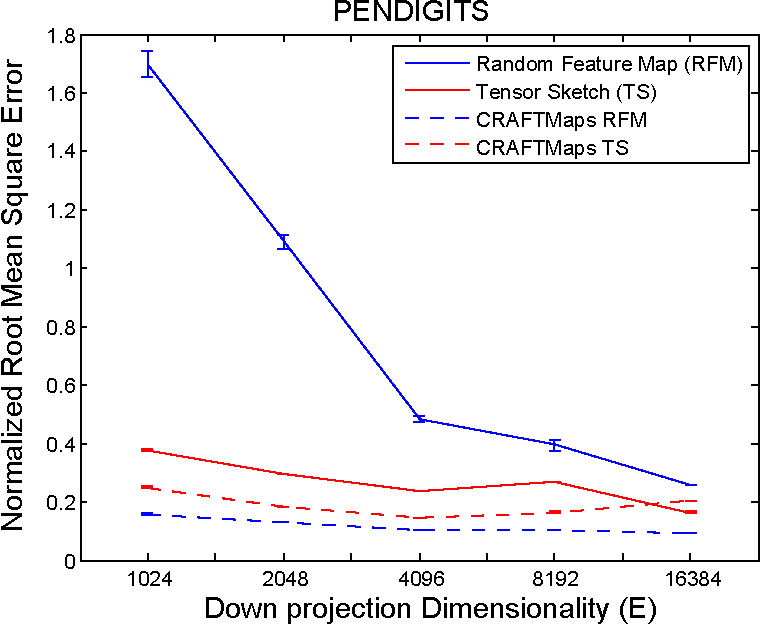
\includegraphics[width=0.75\textwidth]{figures/craftmaps/pendigits}
    \end{center}
\end{frame}
%%%%%%%%%%%%%%%%
\begin{frame}{CRAFTMaps for multi-class learning using ECOCs}
    ECOC idea: use multiple linear regressions to predict the individual coordinates, then assign the class corresponding to the nearest codeword
    \begin{center}
      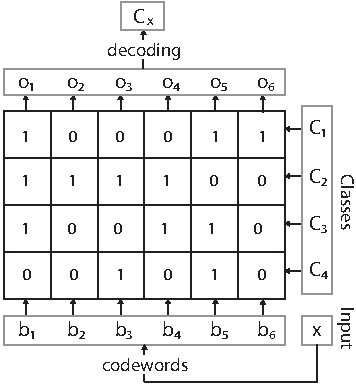
\includegraphics[width=0.5\textwidth]{figures/craftmaps/ecoc_illust}
    \end{center}
\end{frame}

\begin{frame}{Advantages of CRAFTMaps + ECOC}
\begin{enumerate}
 \item Requires only \emph{one pass} over the data
 \item The Hessian is shared, so is only computed once.
 \item The pipeline simple: is a series of matrix-matrix multiplications plus a matrix factorization (Cholesky of the Hessian). Amenable to GPU or distributed computation.
\end{enumerate}
\end{frame}

\begin{frame}
\frametitle{ECOC Test Errors}
\begin{table}[!t]
\begin{center}
\small{
\begin{tabular}{| c|| c| c| c| c| c| c|}
    \hline
    \rowcolor{gray!170}
    $\textrm{\textcolor{white}{e-PENDIGITS}}$ & $\textcolor{white}{2^6}$ & $\textcolor{white}{2^7}$ & $\textcolor{white}{2^8}$ & $\textcolor{white}{2^{9}}$ & $\textcolor{white}{2^{10}}$\\
    \hline
    \hline
    FastFood & $8.74$ & $5.03$ & $3.08$ & $2.85$ & $2.71$\\\hline
    RFF & $5.83$ & $4.25$ & $2.63$ & $2.17$ & $2.08$\\\hline
    KK-RFM & $7.94$ & $3.94$ & $2.85$ & $2.28$ & $1.91$\\\hline
    TS-RFM & $11.20$ & $4.57$ & $2.37$ & $1.80$ & $1.77$\\\hline
    CM KK-RFM & $\textbf{7.43}$ & $\textbf{3.57}$ & $\textbf{2.28}$ & $\textbf{1.97}$ & $\textbf{1.57}$\\\hline
    CM TS-RFM & $8.03$ & $3.80$ & $2.37$ & $2.05$ & $1.74$\\\hline
    Exact & $9.29$ & $3.74$ & $2.74$ & $2.31$ & $2.87$\\
    \hline
  \end{tabular}
}
\caption*{\small{Test classification error percentages on a 10 class problem with 200 ECOCs; r=9 and q=1; the first row is $\mathrm{E}$, and $\mathrm{D}=8 \times \mathrm{E}$.}}
\end{center}
\end{table}
\end{frame}

\begin{frame}
\begin{table}[!t]
\begin{center}
\small{
\begin{tabular}{| c|| c| c| c| c| c| c|}
    \hline
    \rowcolor{gray!170}
    $\textrm{\textcolor{white}{d-COIL100}}$ & $\textcolor{white}{2^{11}}$ & $\textcolor{white}{2^{12}}$ & $\textcolor{white}{2^{13}}$ & $\textcolor{white}{2^{14}}$ & $\textcolor{white}{2^{15}}$\\
    \hline
    \hline
    FastFood & $8.25$ & $7.83$ & $6.80$ & $6.32$ & $5.21$\\\hline
    RFF & $8.14$ & $7.36$ & $6.50$ & $5.97$ & $4.81$\\\hline
    KK-RFM & $11.11$ & $7.55$ & $6.33$ & $5.05$ & $4.83$\\\hline
    TS-RFM & $10.08$ & $7.19$ & $5.69$ & $4.75$ & $4.27$\\\hline
    CM KK-RFM & $8.94$ & $6.86$ & $5.47$ & $4.52$ & $4.08$\\\hline
    CM TS-RFM & $\textbf{8.16}$ & $\textbf{5.97}$ & $\textbf{4.75}$ & $\textbf{4.02}$ & $\textbf{3.96}$\\\hline
    Exact & $9.55$ & $--$ & $--$ & $--$ & $--$\\    
    \hline
  \end{tabular}
}
\caption*{\small{Test classification error percentages on a 100 class problem with 200 ECOCs; r=5 and q=1; the first row is $\mathrm{E}$, and $\mathrm{D}=8 \times \mathrm{E}$.}}
\end{center}
\end{table}
\end{frame}

\begin{frame}
    \frametitle{Time-Accuracy tradeoffs}
    \begin{center}
      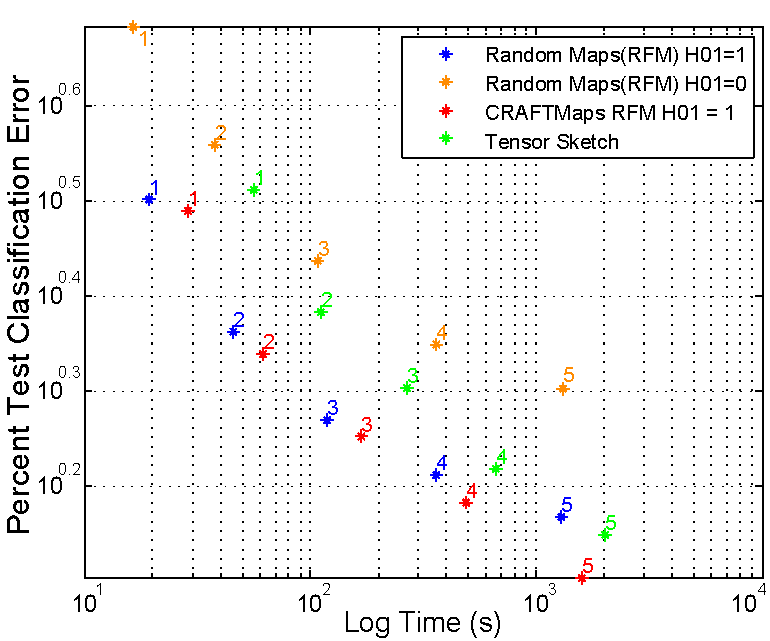
\includegraphics[width=0.75\textwidth]{figures/craftmaps/time_analysis}
    \end{center}
\end{frame}

\section{Word2Vec}

\begin{frame}
Word embeddings are vector representations of words such that simple geometric manipulation of the vectors are semantically meaningful:

\begin{align*}
\mathbf{v}_{\textrm{Paris}} - \mathbf{v}_{\textrm{France}} + \mathbf{v}_{\textrm{Italy}} & \approx \mathbf{v}_{\textrm{Rome}} \\
\mathbf{v}_{\textrm{king}} - \mathbf{v}_{\textrm{man}} + \mathbf{v}_{\textrm{woman}} & \approx \mathbf{v}_{\textrm{queen}}
\end{align*}

Multiple models used to fit word embeddings exhibit similar properties of additivity. All are trained using only
word cooccurrence information taken from a training corpus.

\begin{center}
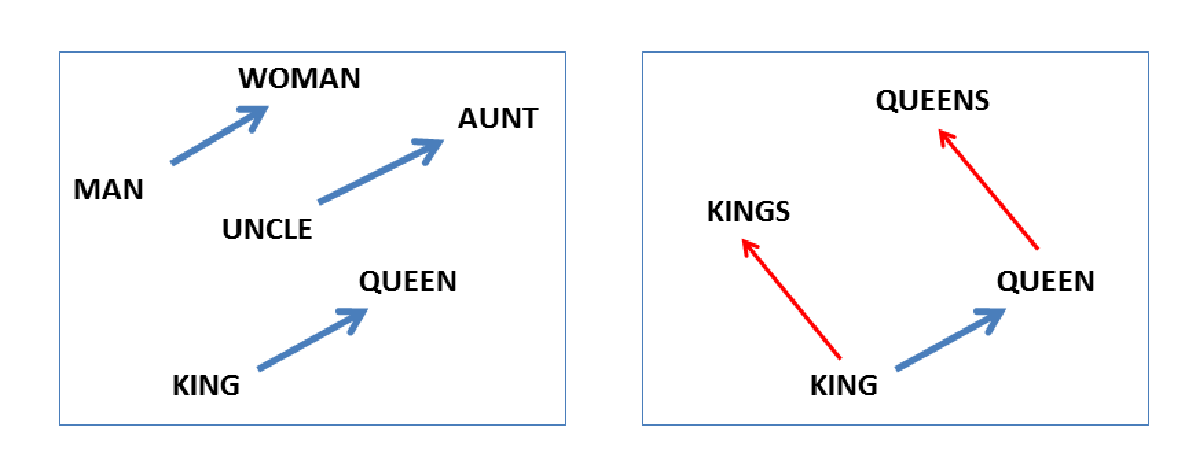
\includegraphics[width=.5\textwidth]{figures/word2vec/plurality}
\\
Recurrent Neural Networks \refer{Mikolov et al. 2013}
\end{center}

\end{frame}

\begin{frame}
\begin{center}
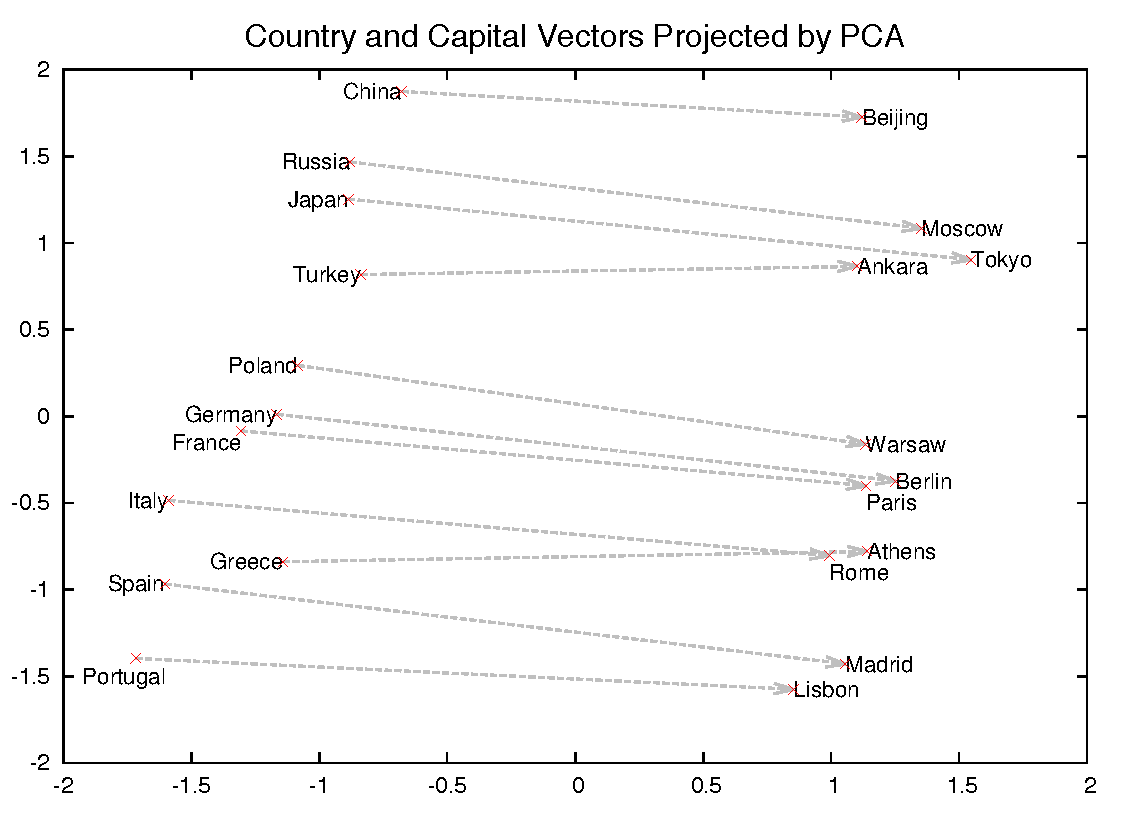
\includegraphics[width=.7\textwidth]{figures/word2vec/capitals}
\\
Word2Vec word embedding \refer{Mikolov et al. 2013}
\end{center}

\begin{block}{Basic Question}
Why do word embeddings have the property of additively capturing semantics? 
\end{block}

\end{frame}

\begin{frame}{Prior Work}
The Rand-Walk model of \refer{Arora et al. 2016}:
\begin{itemize}
  \item \redemphasis{Assumes} the training corpus is generated by a log-linear discourse model
\[
\mathbb{P}(\text{word $w$ occurs at time $t$}\,|\,\mathbf{c}_t) \propto \exp(\langle \mathbf{v}_w, \mathbf{c}_t\rangle )
\]
 \item \redemphasis{Assumes} \emph{a priori} that the discourse vector is a Markov chain with uniform
stationary distribution on the sphere, and the word vectors are isotropic
 \item Establishes that the word vectors can be recovered by factorizing the pointwise mutual information matrix
\[
  \textrm{PMI}(\mathbf{w}_1, \mathbf{w}_2) := \log\left( \frac{p(w_1, w_2)}{p(w_1)p(w_2)} \right) \approx \langle \mathbf{v}_{w1}, \mathbf{v}_{w2} \rangle
\]
\item \greenemphasis{Explains} why analogies can be solved approximately using linear relationships under this model
\item \redemphasis{Does not explain} linear compositionality of word embeddings
\end{itemize}
\end{frame}

\begin{frame}{Our Work}
\begin{itemize}
  \item \greenemphasis{No \emph{a priori} assumptions} on the distribution of the word vectors
  \item Applies to embeddings learned using the canonical \redemphasis{Word2Vec} algorithm
  \item \greenemphasis{Identifies the correct nonlinear operation} for composing multiple words
  \item Identifies an assumption on the corpus that leads to linear 
compositionality and linear solvability of analogies
\end{itemize}
\end{frame}

\begin{frame}{Language models}
Language models model the probability of a sequence of words
\[
\mathbb{P}(w_1, \ldots, w_m)
\]
\begin{itemize}
  \item Useful for speech recognition, machine translation, information retrieval, NLP, ...
  \item Simplest language models, $n$-gram models, are Markov models based on observed frequencies of $n$-tuples
  \item $n$-gram models require an unreasonable amount of data to get accurate models for large $n$ --- the "data-sparsity" problem
\end{itemize}
\end{frame}

\begin{frame}{Neural Language Models}
\begin{itemize}
  \item address the data-sparsity problem with $n$-gram models \refer{Bengio et al. 2003}
  \item learn a word embedding vector $\mathbf{C}(w)$ for each word
  \item maximize the (regularized) log-likelihood of the training data
\[
L(\mathbf{C}, \bm{\theta}) = \frac{1}{T} \sum_t \log \mathbb{P}(w_t\,|\, w_{t-1}, \ldots, w_{t-n+1}) + R(\bm{\theta}),
\]
where 
\begin{multline*}
\mathbb{P}(w_t = i | w_{t-1}, \ldots, w_{t-n+1}) \\
 := g(i, \mathbf{C}(w_{t-1}), \ldots, \mathbf{C}(w_{t-n+1}), \bm{\theta}).
\end{multline*}

\end{itemize}
\end{frame}

\begin{frame}{Neural Language Model of \refer{Bengio et al. 2003}}
\begin{center}
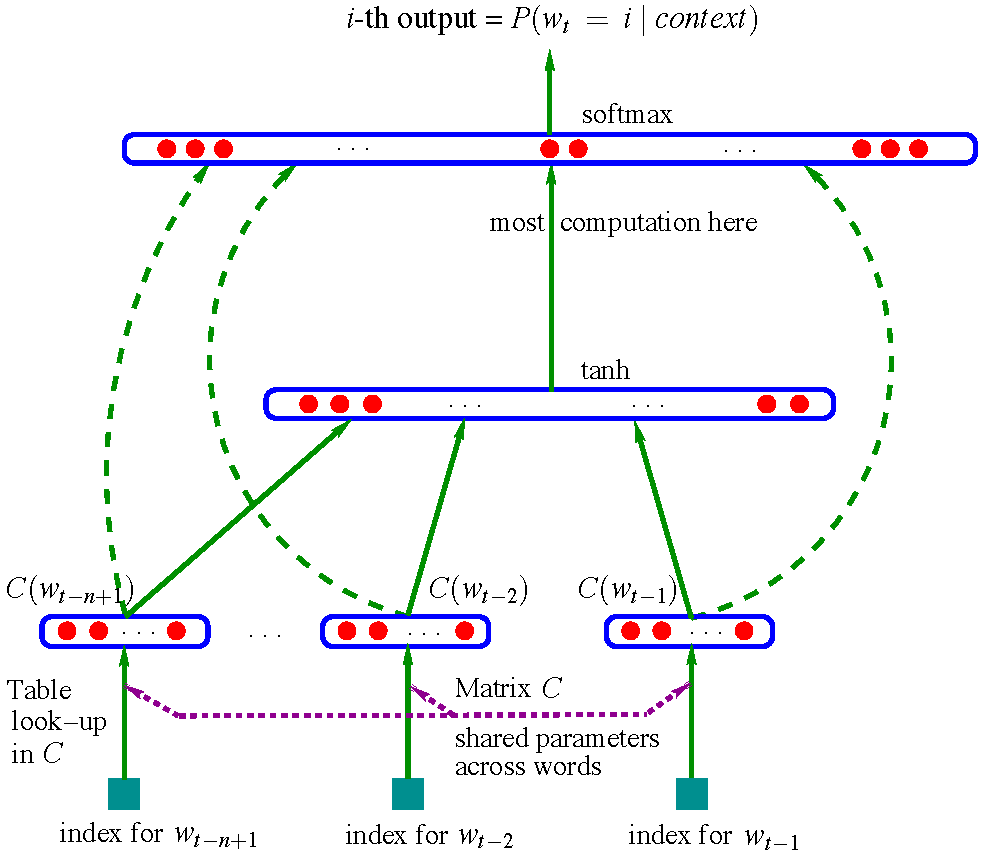
\includegraphics[width=.5\textwidth]{figures/word2vec/bengio-model}
\end{center}

with 
\begin{gather*}
\mathbb{P}(w_t \, |\, w_{t-1}, \ldots, w_{t-n+1}) = \frac{\mathrm{e}^{y_{w_t}}}{\sum_i \mathrm{e}^{y_i}} \\
\mathbf{y} = \mathbf{b} + \mathbf{W}\mathbf{x} + \mathbf{U} \tanh(\mathbf{d} + \mathbf{H}\mathbf{x})
\end{gather*}
\end{frame}

\begin{frame}
Since \refer{Bengio et al. 2003} many similar but simpler and faster models have been proposed. The most well-known:
\begin{itemize}
  \item \redemphasis{Word2Vec} (canonical, hierarchical softmax, negative sampling) (3 papers in 2013; 2825 citations)
  \item \textit{Global Vectors for Word Representation} (2014; 335 citations)
  \item \textit{Noise-contrastive Log-Bilinear models} (2013; 93 citations)
\end{itemize}

These all the share the properties:
\begin{itemize}
  \item Based on co-occurrence counts within a context width
  \item Involve nonlinear dimensionality reduction
\end{itemize}
\end{frame}

\begin{frame}{Canonical (skipgram) Word2Vec}
Based on the distributional hypothesis of Harris and Firth: \emph{words that occur in similar contexts have similar meanings}

\begin{center}
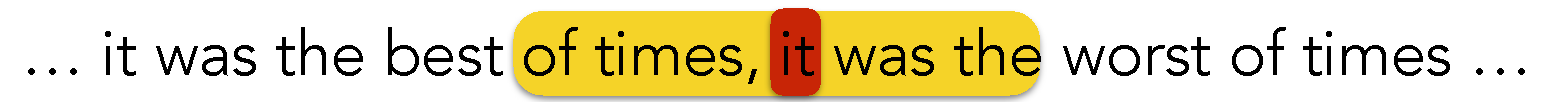
\includegraphics[width=.8\textwidth]{figures/word2vec/context-window}
\end{center}
\begin{tabular}{cl}
\begin{tabular}{c}
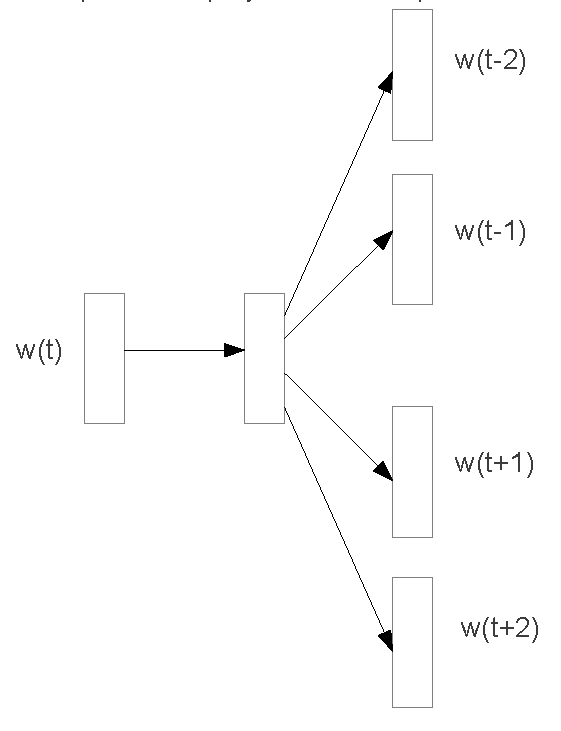
\includegraphics[height=.5\textheight]{figures/word2vec/word2vec-model}
\end{tabular}
&
\begin{tabular}{l}
\parbox{0.5\linewidth}{%
\begin{gather*}
\frac{1}{T}\sum_{i=1}^T \sum_{-c \leq j \leq c, j \neq 0} \log p(w_{t+j} | w_t) \\
p(w_j | w_i) = \frac{\mathrm{e}^{\langle \mathbf{u}_i, \mathbf{v}_j \rangle} }{ \sum_{k=1}^n \mathrm{e}^{\langle \mathbf{u}_i, \mathbf{v}_k \rangle}}
\end{gather*}
}
\end{tabular}
\end{tabular}
\end{frame}

\begin{frame}{Defining compositionality}
  What does it mean for a word to mean the same as a sequence of words, e.g. `king' meaning the same as `royal man'?
  \vskip1em
  Ideally, that all for all context words $c$ 
  \[
    p(c | w_1, \ldots, w_m) = p(c | w).
  \]
  \vskip1em
  But because we have a finite vocabulary, we'll find the best word in the KL-divergence sense:
  \[
    \min_w D_{\textrm{KL}}(p (\cdot | w_1, \ldots, w_m)\, ||\, p(\cdot | w))
  \]
  To solve this, we need to determine
  \[
    p(\cdot| w_1, \ldots w_m)
  \]
\end{frame}

\begin{frame}
  Assuming that the prior distribution over the words is uniform, Bayes rule gives that the probability of a context word given multiple
  predictor words factors as 
  \[
    p( c | w_1, \ldots, w_m) = \Gamma \prod_{i=1}^m p(c|w_i),
  \]
  where the constant $\Gamma$ is independent of $c.$

\begin{block}{Additive compositionality of Word2Vec \refer{G et al. 2016}}
  Assume $p(w)$ is uniform, then given words $w_1, \ldots, w_m$, the word that minimizes 
    \[
      \min_{w} D_{\textrm{KL}}(p (\cdot | w_1, \ldots, w_m)\, ||\, p(\cdot | w))
    \]
    is the word with predictor embedding
    \[
      \mathbf{u}^\star = \sum_{i=1}^m \mathbf{u}_i
    \]
    if such a word exists.
\end{block}
\end{frame}

\begin{frame}{Analogy Answering}
Using Word2Vec (canonical and approximate) models as well as other word
embeddings, \refer{Mikolov et al. 2013} found that multiple simple relationships
were automatically satisfied additively by the learned embeddings.  
\vskip1em
For all these embeddings, to answer analogy questions of the form 
\[
\textcolor{red}{w_a:w_b::w_c:\,?}
\]
e.g., \textcolor{red}{man\,:\,king\,::\,woman\,:\,?},
they used the procedure
\begin{enumerate}
  \item compute 
\[ 
\mathbf{y} = (\mathbf{u}_b - \mathbf{u}_a) + \mathbf{u}_c
\]
  \item find 
\[
w = \textrm{argmax}_w \frac{\langle \mathbf{u}_w, \mathbf{y} \rangle}{ \|\mathbf{u}_w\|_2 \|\mathbf{y}\|_2}
\]
\end{enumerate}

\end{frame}

\begin{frame}
\begin{center}
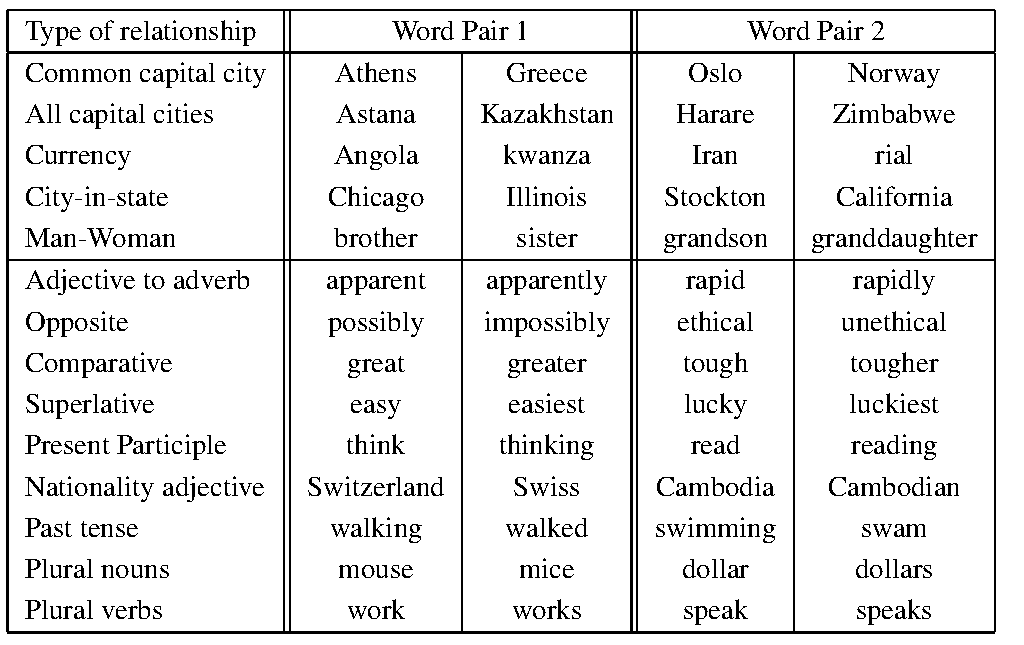
\includegraphics[height=.4\textheight]{figures/word2vec/analogy-pairs}
\\
Examples from the analogies test dataset \refer{Mikolov et al. 2013}
\end{center}

\begin{center}
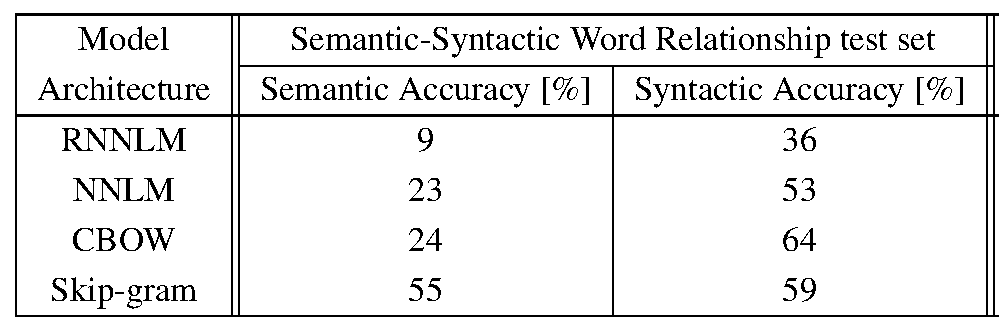
\includegraphics[height=.3\textheight]{figures/word2vec/word2vec-test-results}
\\
Results from training language models using 640-dimensional word vectors on a 320M word corpus with 82K vocabulary \refer{Mikolov et al. 2013}. This is the canonical skip-gram Word2Vec model.
\end{center}

\end{frame}

\begin{frame}{Analogy answering, justified}
  How to answer the analogy \textcolor{red}{China\,:\,Beijing\,::\,USA\,:\,?}
  \vskip1em
  We (conceptually) expand our vocabulary to include relationships as unseen predictor words, e.g.
  \begin{align*}
    p(\cdot\,|\,\textrm{\textcolor{red}{is capital}}, \textrm{China}) &\approx p(\cdot\, | \,\textrm{Beijing}) \\
    p(\cdot\,|\,\textrm{\textcolor{red}{is capital}}, \textrm{USA}) &\approx p(\cdot\, | \,\textrm{Washington, D.C.}) \\
  \end{align*}

  Assume the prior over the words is unifrom. From our results on additive compositionality, we have 
  \begin{align*}
    \mathbf{u}_{\textrm{is capital}} + \mathrm{u}_{\textrm{China}} & \approx \mathbf{u}_{\textrm{Beijing}} \\
    \mathbf{u}_{\textrm{is capital}} + \mathrm{u}_{\textrm{USA}} & \approx \mathbf{u}_{\textrm{Washington, D.C.}}
  \end{align*}
  So it follows that 
  \[
    \mathrm{u}_{\textrm{USA}} + \left( \mathrm{u}_{\textrm{Beijing}} - \mathrm{u}_{\textrm{China}}\right) \approx \mathbf{u}_{\textrm{Washington, D.C.}}
  \]
  is the desired solution

\end{frame}

\begin{frame}{Nonuniform priors}
  In general, the prior distribution is nonuniform (Zipf!). In this case,
  \[
    p( c | w_1, \ldots, w_m) = \Gamma_c \prod_{i=1}^m p(c | w_i)
  \]
  and the operation that gives compositionality nonlinear.

  \begin{block}{Nonlinear compositionality \refer{G et al. 2016}}
  Given words $w_1, \ldots, w_m$, the word that minimizes 
    \[
      \min_{w} D_{\textrm{KL}}(p (\cdot | w_1, \ldots, w_m)\, ||\, p(\cdot | w))
    \]
    is the word whose predictor embedding satisfies
    \[
      \mathbb{E}[\mathbf{v}_c \,|\, w_1, \ldots, w_m] = \mathbb{E}[\mathbf{v}_c \,|\, w]
    \]
    if such a word exists.
  \end{block}
\end{frame}
\begin{frame}
  Word2Vec's objective can be specified entirely in terms of the co-occurence matrix $\mathbf{G}$ and embedding matrices $\mathbf{U}, \mathbf{V}$:
  \begin{itemize}
    \item $G_{ij}$ is the number of times $w_i$ and $w_j$ co-occur within a context window in the corpus
    \item The rows of $\mathbf{U}$ and $\mathbf{V}$ give the embeddings for $w_i$
  \end{itemize}

  \begin{block}{Batch Formulation of Word2Vec \refer{G et al. 2016}}
    Word2Vec seeks maximizers $\mathbf{U}$ and $\mathbf{V}$ of 
    \[
    \max_{\mathbf{U}, \mathbf{V}} \textrm{Trace}(\mathbf{G} \mathbf{U} \mathbf{V}^T) - \mathbf{1}^T \mathbf{G} \log( \mathrm{e}^{\mathbf{U} \mathbf{V}^T} \mathbf{1}).
  \]
  \end{block}

  This follows directly from expanding out the objective stated previously. Note that
  \[ (\mathbf{G}\mathbf{1})_i = G_i \propto p(w_i) \]
  So Word2Vec is trying to maximize a matrix inner-product subject to an entropy regularization.
\end{frame}

\begin{frame}
  Define the weighted row-normalized KL-divergence of two matrices by
  \[
    D^{\omega}_{\mathrm{KL}}(\mathbf{A}\,||\,\mathbf{B}) = \sum_i \omega_i  D_{\mathrm{KL}}(\hat{\mathbf{a}}_i\,||\,\hat{\mathbf{b}}_i)
  \]

  Normalizing the rows of $\mathbf{G}$ yields a collection of empirical distributions $p(w_j | w_i)$ characterizing each word $w_i.$ Likewise,
  normalizing the rows of $\mathrm{e}^{\mathbf{UV}^T}$ yields a collection of probability distributions. Word2Vec attempts to
  minimize a weighted sum of the divergence between the corresponding distributions.

  \begin{block}{KL-divergence minimization formulation of Word2Vec \refer{G et al. 2016}}
    Word2Vec minimizes 
    \[
      D^{\omega}_{\mathrm{KL}}\left(\mathbf{G}\,||\,\mathrm{e}^{\mathbf{UV}^T}\right)
    \]
    for $\omega = \mathbf{G}\mathbf{1}.$
  \end{block}

  This follows from observing that maximizing likelihood is the same as minimizing KL divergence.
\end{frame}

\begin{frame}
  According to the principle of sufficient dimensionality reduction \refer{Globerson
    et al. 2003}, given co-occurence information $\mathbf{G}$ for two discrete random
  variables $X$ and $Y$ with $n$ and $m$ states respectively, a model of the form
  \[
    \mathbf{G} = \mathrm{e}^{\mathbf{UV}^T}, \quad \mathbf{U} \in \mathbb{R}^{n \times d} \text{ and } \mathbf{V} \in \mathbb{R}^{m \times d}
  \]
  preserves the maximum amount of mutual information between $X$ and $Y$ and this model can be obtained by minimizing
  \[
    D_{\textrm{KL}}(z_G^{-1} \mathbf{G} \,||\, z_e^{-1} \mathrm{e}^{\mathbf{UV}^T}).
  \]
  That is, rescale $\mathbf{G}$ and $\mathrm{e}^{\mathbf{UV}^T}$ to be \emph{joint} probability distributions over $(X, Y)$
  and find the closest exponential factorization in the KL divergence.


\end{frame}

\begin{frame}{Word2Vec fits SDR}
  \begin{block}{\refer{G et al. 2016}}
    Word2Vec fits an SDR model.
  \end{block}

  \refer{Globerson et al. 2003} shows that the SDR model performs well at text categorization and information retrieval, but fitting an SDR model is expensive. 
  After each update to $\mathbf{U}, \mathbf{V}$, the normalizer $z_e = \sum_{ij} \mathrm{e}^{\mathbf{UV}^T}$ must be recalculated.
  \vskip1em
  This suggests fitting Word2Vec-like models instead, which only compute row-wise normalization constants. 
\end{frame}

\begin{frame}{Multi-label classification}
\end{frame}

\section{NLA in Spark}
\begin{frame}
\vfill
\begin{beamercolorbox}[center]{}
\Large \textsc{Low-Rank approximations in Spark}
\end{beamercolorbox}
\vfill
\end{frame}

\begin{frame}
\begin{center}
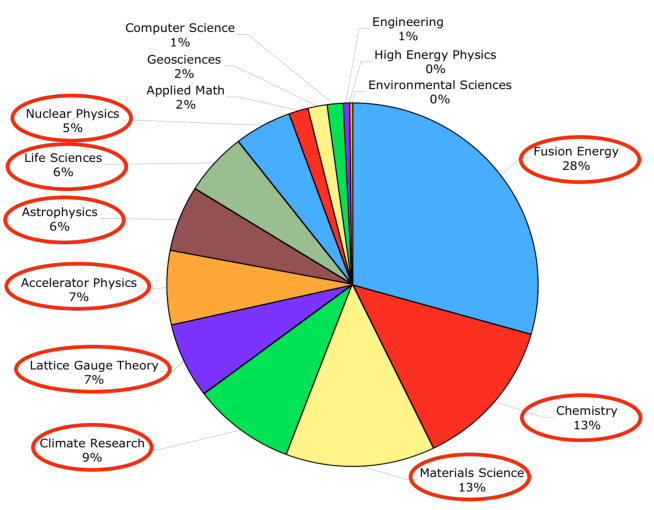
\includegraphics[width=.5\textwidth]{figures/spark/NERSC_usage}
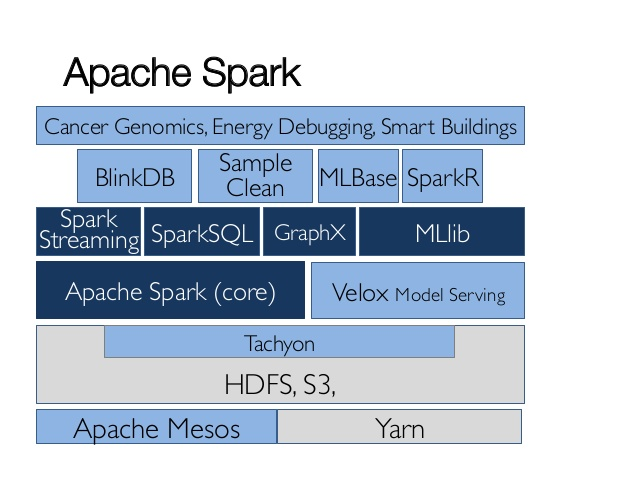
\includegraphics[width=.5\textwidth]{figures/spark/bdas-stack.jpg}
\end{center}
I am interested in adding linear algebra++ algorithms to the Berkeley Data Analytics Stack.
\vskip1em
Collaborators at NERSC are investigating Spark as a unified platform for data analytics pipelines with diverse scientific inputs.
\vskip1em
Collaborators at Cray, Inc. are interested in Spark because of market demand, want to understand performance concerns.
\end{frame}

\begin{frame}
  \begin{center}
  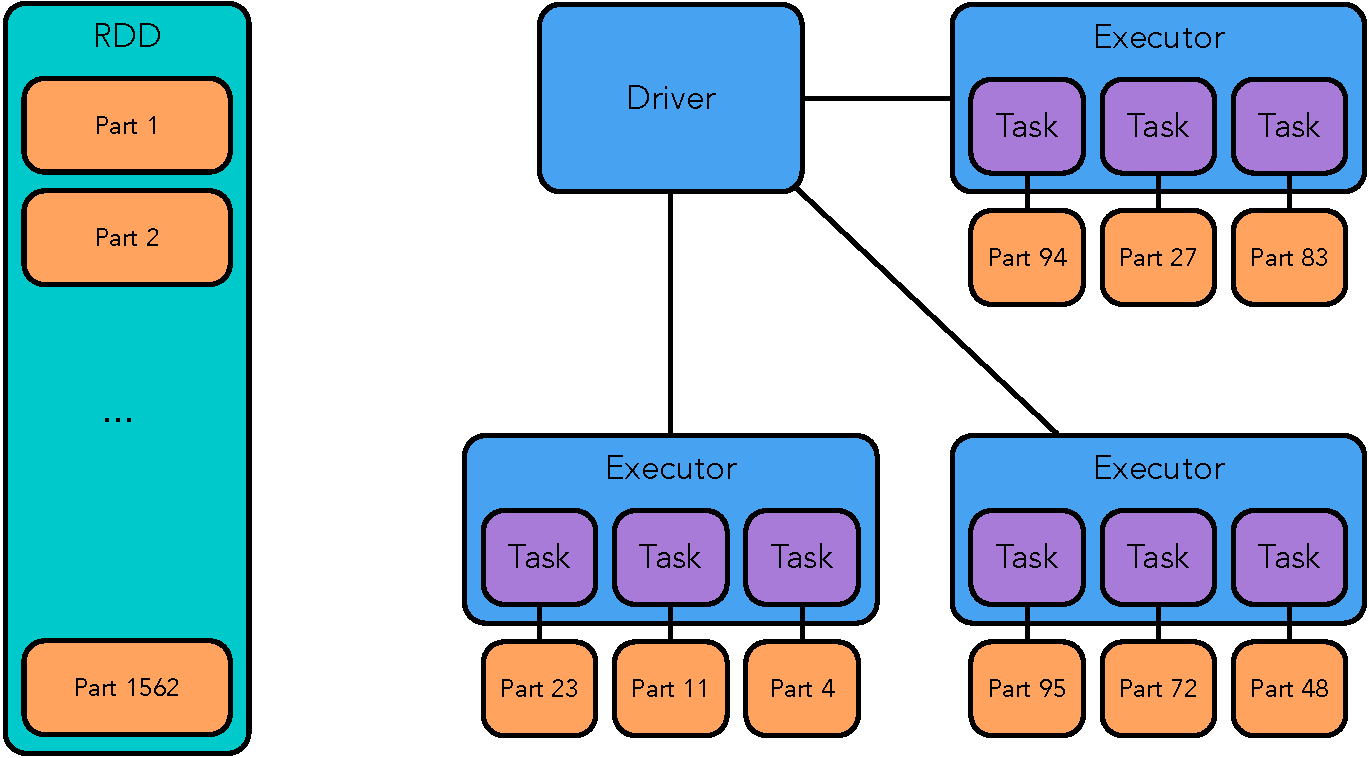
\includegraphics[width=0.75\textwidth]{figures/spark/spark-driver-rdd-architecture}
\end{center}
\begin{itemize}
  \item Spark is a distributed programming environment that implements a data-parallel programming model. 
  \item The \emph{driver} forms the computational DAG, schedules tasks on the \emph{executors}
  \item All data is stored as \emph{Resilient Distributed Datasets} (RDDs) that
    are partitioned across the executors and optionally cached in memory. 
\end{itemize}
\end{frame}

\begin{frame}
  \begin{center}
    \includegraphics[width=0.9\textwidth]{figures/spark/spark-staging}
  \end{center}
  \begin{itemize}
    \item Each \emph{job} (DAG) is broken into \emph{stages}
    \item Stages are divided into parallel, independent \emph{tasks}
    \item Communication happens only between stages
  \end{itemize}
\end{frame}

\begin{frame}
  Spark's performance generally depends on \textbf{problem scale} and \textbf{level of parallelism} (DAG complexity),
  as well as the amount of communication required, as measured in \textbf{stages}. 
  \begin{center}
  \includegraphics[width=0.8\textwidth]{figures/spark/spark-usage}
  \end{center}
\end{frame}

\begin{frame}{Our Goals}
  \begin{itemize}
    \item \redemphasis{Provide implementations} of low-rank factorizations (PCA, NMF, and randomized CX) in Spark
    \item Successfully apply low-rank matrix factorizations to \redemphasis{TB-scale scientific datasets} in Spark
    \item Understand \redemphasis{Spark performance on commodity clusters vs HPC platforms}
    \item \redemphasis{Quantify the gaps} between highly-tuned C+MPI and Spark implementations
    \item \redemphasis{Investigate the scalability} of Spark for linear algebra on HPC platforms
  \end{itemize}
\end{frame}

\begin{frame}{Datasets}
\begin{table}[ht]
\centering
\begin{tabular}{p{2.2cm}lllll@{}}
\toprule
\textbf{Science Area} & \textbf{Format/Files} & \textbf{Dimensions} & \textbf{Size}  \\ \midrule
Daya Bay & HDF5/1      &   $1,099,413,914 \times 192$         & 1.6TB \\
Ocean              & HDF5/1      &  $6,349,676 \times 46,715$          & 2.2TB \\
Atmosphere           & HDF5/1       & $26,542,080 \times 81,600$           & 16TB \\ \bottomrule
\end{tabular}
\end{table}

\vskip1em
  \textcolor{dgreen}{Daya Bay} --- neutrino sensor array measurements; used for NMF
\vskip1em
  \textcolor{dgreen}{Ocean and Atmosphere} --- climate variables (ocean temperature, atmospheric humidity) measured on a 3D grid at 3 or 6 hour intervals over about 30 years; used for PCA
\end{frame}

\begin{frame}{Running times}
On the NERSC Cori supercomputer (Cray XC40):
\begin{center}
\begin{itemize}
  \item 1630 compute nodes
  \item 128 GB/node
  \item 32 2.3GHz Haswell cores/node
\end{itemize}
\end{center}

\centering
\resizebox{\columnwidth}{!}{
\begin{tabular}{|c|c|c|c|c|c|} \hline
Algo & Size & \# Nodes & MPI Time (s) & Spark Time (s)\\ \hline
\multirow{3}{*}{NMF} & \multirow{3}{*}{1.6 TB} & $50$ & $66$ & $278$\\
{} & {} & $100$  & $45$ & $207$\\
{} & {} & $300$ & $30$ & $70$\\ \hline
\multirow{4}{*}{PCA} & \multirow{3}{*}{2.2 TB} & 100 & 94 & 934\\
 {} & {} & 300 & 60 & 827\\
 {} & {} & 500 & 56 & 1160\\ \cline{2-5}
 {} & {16 TB} & {MPI: 1600 Spark: 1522} & 160 & 4175 \\ \hline
% {} & \multirow{3}{*}{Spark} & {} & $221$ & $122$ & $032$\\
% {} & {} & \multirow{2}{*}{$311$} & $212$ & $131$ & $023$\\
% {} & {} & {} & {} & $113$ & $050$\\
\end{tabular}
}
\end{frame}

\begin{frame}{Performance Gaps}
For data analysis, performance with IO is more relevant. For HPC tasks, performance without IO is more relevant.
\begin{table}[t]
\begin{center}
\resizebox{\columnwidth}{!}{
\begin{tabular}{|c|c|c|c|} \hline
Algo & \# Nodes & Gap with I/O & Gap without I/O\\ \hline
\multirow{3}{*}{NMF} & $50$ & $4\times$ & $21.2 \times$\\
{} & $100$  & $4.6\times$ & $14.9\times$\\
{} & $300$ & $2.3\times$ & $15.7\times$\\ \hline
\multirow{4}{*}{PCA} & 100 & $10.2\times$ & $12.6\times$\\
 {} & 300 & $14.5\times$ & $24.7\times$\\
 {} & 500 & $22\times$ & $39.3\times$\\ \cline{2-4}
 {} & {MPI: 1600 Spark: 1522} & $26\times$ & $43.8\times$\\ \hline
\end{tabular}
}
\end{center}
\end{table}
\end{frame}

\begin{frame}{PCA algorithm}
The rank-$k$ truncated PCA of a matrix $\mathbf{A}$ with centered rows is given by
\[
\mathbf{A}_k = \mathbf{U}_k \bm{\Sigma}_k \mathbf{V}_k^T
\]
where $\bm{\Sigma}_k$ contains the top $k$ singular values of $\mathbf{A}$ and $\mathbf{U}_k, \mathbf{V}_k$ 
contain the corresponding singular vectors.
\vskip1em
We use the following algorithm to compute $\mathbf{A}_k$ when $\mathbf{A}$ is tall and skinny:
 \begin{enumerate}
   \item Compute $\mathbf{V}_k$ as the top $k$ eigenvectors of $\mathbf{A}^T \mathbf{A}$ using a Lanczos eigensolver with distributed matrix-vector multiplies. 
   \item Compute $\mathbf{A V}_k$ and collect on the driver.
   \item On the driver, compute the SVD of $\mathbf{A V}_k$ to get $\mathbf{U}_k$ and $\bm{\Sigma}_k.$
 \end{enumerate}
\end{frame}

\begin{frame}{Scaling for PCA}
\begin{figure}[th!]
\centering
\includegraphics[width=.45\textwidth]{figures/spark/mpi_pca.png}
\includegraphics[width=.5\textwidth]{figures/spark/spark_pca.png}
\\
Running time breakdown of PCA on 2.2TB Ocean data at node counts of 100, 300 and 500. MPI 
is to the left, Spark to the right.
\end{figure}
\end{frame}

\begin{frame}
\begin{figure}[th!]
\centering
\includegraphics[width=.72\textwidth]{figures/spark/hero_run_summary.png}
\\
Running time comparison of MPI PCA and Spark PCA for the 1600 node run.
\end{figure}
\end{frame}

\begin{frame}
\begin{figure}[th!]
\centering
\includegraphics[height=.85\textheight]{figures/spark/spark_pca_hero_timeline.png}
\\
A timeline of tasks on one node during a multiply-Gramian stage during the 16TB PCA run.
\end{figure}
\end{frame}

\begin{frame}{NMF Algorithm}
NMF is used when observations are positive, and assumed to be positive linear combinations of basis vectors
(e.g. medical imaging modalities, hyperspectral imaging)
\vskip1em
The NMF factorization is given by
\[
(\mathbf{W}, \mathbf{H}) = \text{argmin}_{\substack{\mathbf{W} \geq 0 \\ \mathbf{H} \geq 0}} \|\mathbf{A} - \mathbf{W}\mathbf{H}\|_F^2
\]
\vskip1em
We use the one-pass approach of \refer{Benson et al. 2014} that assumes $\mathbf{W}$ can be selected from the columns of $\mathbf{A}$. Then the problem
reduces to that of taking a tall-skinny QR of $\mathbf{A}$ and postprocessing the $\mathbf{R}$ factor, on the driver, to choose those columns.
\end{frame}

\begin{frame}
When $\mathbf{A}$ is tall and skinny, its QR factorization can be computed efficiently using the TSQR algorithm:
\begin{figure}[h!]
\includegraphics[height=.7\textheight]{figures/spark/tsqr}
\end{figure}
This uses a tree reduction, so communicates minimally between stages, and requires only one pass over the matrix.
\end{frame}

\begin{frame}{Scaling for NMF}
\begin{figure}[th!]
\centering
\includegraphics[width=.5\textwidth]{figures/spark/mpi_nmf_big_scale.png}
\includegraphics[width=.5\textwidth]{figures/spark/spark_nmf.png}
\\
Running time breakdown of NMF on 1.6TB Daya Bay data at node counts of 50, 100 and 300. MPI 
is to the left, Spark to the right.
\end{figure}
\end{frame}

\begin{frame}{Lessons learned}
  \begin{itemize}
    \item Even with favorable data (tall and skinny) and well-adapted algorithms, \redemphasis{Spark is 2x-10x slower than MPI when IO is included, 10x-40x when IO is not included
}
  \item \redemphasis{Spark overheads are orders of magnitude higher than the computations} 

  \item The straggler effect from large overheads means the \redemphasis{impact of overheads increases as concurrency does}

  \item This gap suggests it is worthwhile to \redemphasis{interface MPI-based codes with Spark or augment Spark's communication model}
  \end{itemize}
\end{frame}

\begin{frame}{Recap}
  We considered four instances of low-rank approximation:
  \begin{itemize}
    \item \greenemphasis{SPSD Sketches}, where we obtained bounds for the approximation error of randomized SPSD sketches
    \item \greenemphasis{Polynomial Random Features}, where guidance was
      provided for the number of features needed to achieve low kernel
      approximation error, and the theory motivated an effective algorithm for
      futher reducing the number of features needed 
    \item \greenemphasis{Word2Vec}, where we offered a rigorous justification for the observation that word embeddings capture semantics additively, and 
      the theory led to a faster algorithm for fitting SDR models.
    \item \greenemphasis{Low-rank factorization in Spark}, where we quantified the slow-down of large-scale low-rank factorization algorithms in Spark
      relative to their performance in C+MPI.
  \end{itemize}
\end{frame}
\end{document}
